%%%%%%%%%%%%%%%%%%%%%%%%%%%%%%%%%%%%%%%%%%%%%%%%%%%%%%%%%%%%%%%%%
% Contents: Main Input File of the LaTeX2e Introduction
% $Id$
%%%%%%%%%%%%%%%%%%%%%%%%%%%%%%%%%%%%%%%%%%%%%%%%%%%%%%%%%%%%%%%%%
% lshort.tex - The not so short introduction to LaTeX   
%                                                      by Tobias Oetiker
%                                                     oetiker@ee.ethz.ch
%
%                           based on LKURTZ.TEX Uni Graz & TU Wien, 1987
%-----------------------------------------------------------------------
%
% To compile lshort, you need TeX 3.x, LaTeX and makeindex
%
% The sources files of the Intro are:
%      lshort.tex (this file),
%      titel.tex, contrib.tex, biblio.tex
%      things.tex, typeset.tex, math.tex, lssym.tex, spec.tex,
%      lshort.sty, fancyheadings.sty
%
% Further the  verbatim.sty and the layout.sty 
% from the LaTeX Tools distribution is
% required.
%
%
% To print the AMS symbols you need the AMS fonts and the packages
% amsfonts, eufrak and eucal from (AMS LaTeX 1.2)
%
% ---------------------------------------------------------------------

%%%%%%%%%%%%%%%%%%%%%%%%%%%%%%%%%%%%%%%%%%%%%%%%%%%%%%%%%%%%%%%%%
% Contents: Who contributed to this Document
% $Id$
%%%%%%%%%%%%%%%%%%%%%%%%%%%%%%%%%%%%%%%%%%%%%%%%%%%%%%%%%%%%%%%%%
\begin{small} 
  \noindent Copyright \copyright 1995-2010 Tobias Oetiker and Contributors.  All rights reserved.
 
  This document is free; you can redistribute it and/or modify it
  under the terms of the GNU General Public License as published by
  the Free Software Foundation; either version 2 of the License, or
  (at your option) any later version.
  
  This document is distributed in the hope that it will be useful, but
  \emph{without any warranty}; without even the implied warranty of
  \emph{merchantability} or \emph{fittness for a particular purpose}\@.  See the GNU
  General Public License for more details.
  
  You should have received a copy of the GNU General Public License
  along with this document; if not, write to the Free Software
  Foundation, Inc., 675 Mass Ave, Cambridge, MA 02139, USA.

\end{small}

\chapter{Thank you!}
\noindent Much of the material used in this introduction comes from an
Austrian introduction to \LaTeX\ 2.09 written in German by:
\begin{verse}
\contrib{Hubert Partl}{partl@mail.boku.ac.at}%
{Zentraler Informatikdienst der Universit\"at f\"ur Bodenkultur Wien}
\contrib{Irene Hyna}{Irene.Hyna@bmwf.ac.at}%
   {Bundesministerium f\"ur Wissenschaft und Forschung Wien}
\contrib{Elisabeth Schlegl}{no email}%
   {in Graz}
\end{verse}

If you are interested in the German document, you can find a version
updated for \LaTeXe{} by J\"org Knappen at
\CTAN|info/lshort/german|

\newpage \noindent The
following individuals helped with corrections, suggestions and
material to improve this paper. They put in a big effort to help me
get this document into its present shape. I would like to
sincerely thank all of them. Naturally, all the mistakes you'll find
in this book are mine. If you ever find a word that is spelled
correctly, it must have been one of the people below dropping me a
line.

{ \flushleft\small
Eric~Abrahamsen,        %eric@ericabrahamsen.net
Rosemary~Bailey,        %r.a.bailey@qmw.ac.uk 0.2
Marc~Bevand,            % <bevand_m@epita.fr>
Friedemann~Brauer,      %fbrauer@is.dal.ca 3.4
Barbara~Beeton,         %bnb@ams.org
Salvatore~Bonaccorso,   % bonaccos@ee.ethz.ch
Jan~Busa,               % <busaj@ccsun.tuke.sk>
Markus~Br\"uhwiler,     % <m.br@switzerland.org>
Pietro~Braione,         % <braione@elet.polimi.it>
David~Carlisle,         %GONE carlisle@cs.man.ac.uk 1.0
Jos\'e~Carlos~Santos,   % <jcsantos@fc.up.pt>
Neil~Carter,            % N.Carter@Swansea.ac.uk
Mike~Chapman,           %chapman@eeh.ee.ethz.ch 3.16
Pierre~Chardaire,       % <pc@sys.uea.ac.uk
Christopher~Chin,       %chris.chin@rmit.edu.au 3.1
Carl~Cerecke,           %cdc@cosc.canterbury.ac.nz>
Chris~McCormack,        %GONE chrismc@eecs.umich.edu 0.1
Diego~Clavadetscher,    % DC@clavatax.ch
Wim~van~Dam,            %GONE wimvdam@cs.kun.nl 2.2
Jan~Dittberner,         %jan@jan-dittberner.de 3.15
Michael~John~Downes,    %<mjd@ams.org> 14 Oct 1999
Matthias~Dreier,        %dreier@ostium.ch
David~Dureisseix,       %dureisse@lmt.ens-cachan.fr 1.1
Eilinger~August,        % <eaugust@student.ethz.ch>
Elliot,                 %GONE enh-a@minster.york.ac.uk 1.1
Rockrush~Engch,         %niatlantice@gmail.com
Hans~Ehrbar,            %ehrbar@econ.utah.edu
Daniel~Flipo,           %Daniel.Flipo@univ-lille1.fr
David~Frey,             %david@eos.lugs.ch 2.2
Hans~Fugal,             %hans@fugal.net
Robert~Funnell,         %<robert.funnell@mcgill.ca>
Robin~Fairbairns,       %Robin.Fairbairns@cl.cam.ac.uk 0.2 1.0
J\"org~Fischer,        %j.fischer@xpoint.at 3.16
Erik~Frisk,             %frisk@isy.liu.se 3.4
Mic~Milic~Frederickx,   % <mic.milic@web.de>
Frank,                  %frank@freezone.co.uk 11 Feb 2000
Kasper~B.~Graversen,    % <kbg@dkik.dk>
Arlo~Griffiths,         % <A.Griffiths@let.leidenuniv.nl>
Alexandre~Guimond,      %guimond@IRO.UMontreal.CA 0.9
Andy~Goth,              % <unununium@openverse.com>
Cyril~Goutte,           %goutte@ei.dtu.dk 2.1 2.2
Greg~Gamble,            %gregg@maths.uwa.edu.au 2.2
Frank~Fischli,          % <fischlifaenger@gmx.ch>
Morten~H�gholm,		% morten.hoegholm@latex-project.org
Neil~Hammond,           %nfh@dmu.ac.uk 0.3
Rasmus~Borup~Hansen,    %GONE rbhfamos@math.ku.dk 0.2 0.9 0.91 0.92 1.9.9
Joseph~Hilferty,        % <hilferty@fil.ub.es>
Bj\"orn Hvittfeldt,     %bjorn@hvittfeldt.com 3.13
Martien~Hulsen,         %M.A.Hulsen@WbMt.TUDelft.NL 1.0 1.1
Werner~Icking,          %<Werner.Icking@gmd.de> 3.1
Jakob,                  %diness@get2net.dk
Eric~Jacoboni,          %GONE jacoboni@enseeiht.fr 0.1 0.9
Alan~Jeffrey,           %alanje@cogs.sussex.ac.uk 0.2
Byron~Jones,            %bj@dmu.ac.uk 1.1
David~Jones,            %GONE djones@CA.McMaster.dcss.insight 1.1
Nils~Kanning,           % <nils@kanning.de>
Tobias~Krewer,          %tobias.krewer@googlemail.com
Johannes-Maria~Kaltenbach, %<kaltenbach@zeiss.de> 3.01
Andrzej~Kawalec,        %GONE akawalec@prz.rzeszow.pl 1.9.9
Sander~de~Kievit,       %Skievit@ucu.uu.nl
Alain~Kessi,            %ALAIN_KESSI@HOTMAIL.COM 2.2
Christian~Kern,         %ck@unixen.hrz.uni-oldenburg.de 2.1
Tobias~Klauser,		%tklauser@access.unizh.ch 4.17
J\"org~Knappen,         %knappen@vkpmzd.kph.uni-mainz.de 0.1
Kjetil~Kjernsmo,        %<kjetil.kjernsmo@astro.uio.no> 3.2
Michael~Koundouros,     % <mkoundouros@hotmail.com>
Matt~Kraai,             % <Matt.Kraai@amo.abbott.com>
Maik~Lehradt,           %greek@uni-paderborn.de 0.1
R\'emi~Letot,           % <r_letot@yahoo.com>
Flori~Lambrechts,       % <f.lambrechts@softhome.net>
Mike~Lee,               % rmrstar@gmail.com
Axel~Liljencrantz,	% <Axel.Liljencrantz@byv.kth.se>
Johan~Lundberg,         %p99jlu@physto.se
Alexander~Mai,          %Alexander.Mai@physik.tu-darmstadt.de 3.8
Hendrik~Maryns,         %hendrik.maryns@ugent.be
Martin~Maechler,        %<maechler@stat.math.ethz.ch> 2.2
Aleksandar~S~Milosevic, % <aleksandar.milosevic@yale.edu>
Henrik~Mitsch,          % <Henrik.Mitsch@gmx.at>
Claus~Malten,           %GONE <ASI138%BITNET.DJUKFA11@BITNET.CEARN> 1.1
Kevin~Van~Maren,        % <vanmaren@fast.cs.utah.edu>  24 Nov 1999
Stefan~M.~Moser,        % stefan.moser@ieee.org 
Richard~Nagy,           % r.nagy@nameshield.net
Philipp~Nagele,         % Philipp.Nagele@t-systems.com
Lenimar~Nunes~de~Andrade, % <lenimar@mat.ufpb.br> Fri, 12 Nov 1999
I.~J.~Vera~Mar\'un,    % I.J.Veramarun@ewi.utwente.nl
Manuel~Oetiker,         % manuel@oetiker.ch
Urs~Oswald,             % osurs@bluewin.ch
Lan~Thuy~Pham,          %<lan.thuy.pham@gmail.com>
Martin~Pfister,		% m@rtinpfister.ch
Breno~Pietracci,        % <bpietracci@gmail.com>
Demerson~Andre~Polli,   % polli@linux.ime.usp.br
Nikos~Pothitos,		% <n.pothitos@di.uoa.gr>
Maksym~Polyakov         % <polyama@myrealbox.com>
Hubert~Partl,           %partl@mail.boku.ac.at 0.2 1.1
John~Refling,           %refling@sierra.lbl.gov 0.1 0.9
Mike~Ressler,           %ressler@cougar.jpl.nasa.gov 0.1 0.2 0.9 1.0 1.9.9
Brian~Ripley,           %ripley@stats.ox.ac.uk 2.1
Young~U.~Ryu,           %ryoung@utdallas.edu 2.1
Bernd~Rosenlecher,      %9rosenle@informatik.uni-hamburg.de 10 Feb 2000
Kurt~Rosenfeld,		%kurt@isis.poly.edu
Chris~Rowley,           %C.A.Rowley@open.ac.uk 0.91
Axel~Kielhorn,          % a.kielhorn@web.de
Risto~Saarelma,         %risto.saarelma@cs.helsinki.fi
Jordi~Serra~i~Solanich, %solanich@gmail.com
Hanspeter~Schmid,       %schmid@isi.ee.ethz.ch
Craig~Schlenter,        %cschle@lucy.ee.und.ac.za 0.1 0.2 0.9
Gilles~Schintgen,       %gschintgen@internet.lu
Baron~Schwartz,         % <bps7j@cs.virginia.edu>      
Christopher~Sawtell,    %<csawtell@xtra.co.nz> 1 Sep 1999
Miles~Spielberg,        %zeibach@hotmail.com
Matthieu~Stigler,       % table row height
Geoffrey~Swindale,      % <geofftswin@ntlworld.com>
Laszlo~Szathmary,       % <szathml@delfin.klte.hu>
Andr{\'a}s~Salamon,        % Andras.Salamon@comlab.ox.ac.uk
Boris~Tobotras,         % <tobotras@jet.msk.su>
Josef~Tkadlec,          %tkadlec@math.feld.cvut.cz 2.0 2.2
Scott~Veirs,            %scottv@ocean.washington.edu
Didier~Verna,           %verna@inf.enst.fr 2.2
Fabian~Wernli,          %wernli@iap.fr 3.2
Carl-Gustav~Werner,     % <Carl-Gustav.Werner@math.lu.se> 11 Oct 1999,3.16
David~Woodhouse,        % <dwmw2@infradead.org> 3.16
Chris~York,             % <c.s.york@Cummins.com>  21 Nov 1999
Fritz~Zaucker,          %zaucker@ee.ethz.ch 3.0
Rick~Zaccone,           %zaccone@bucknell.edu 2.2
and Mikhail~Zotov.      %zotov@eas.npi.msu.su 3.1

}

\vspace*{\stretch{1}}



\pagebreak
\endinput
%

% Local Variables:
% TeX-master: "lshort2e"
% mode: latex
% mode: flyspell
% End:

%%%%%%%%%%%%%%%%%%%%%%%%%%%%%%%%%%%%%%%%%%%%%%%%%%%%%%%%%%%%%%%%%
% Contents: Who contributed to this Document
% $Id$
%%%%%%%%%%%%%%%%%%%%%%%%%%%%%%%%%%%%%%%%%%%%%%%%%%%%%%%%%%%%%%%%%

% Because this introduction is the reader's first impression, I have
% edited very heavily to try to clarify and economize the language.
% I hope you do not mind! I always try to ask "is this word needed?"
% in my own writing but I don't want to impose my style on you... 
% but here I think it may be more important than the rest of the book.
% --baron

\chapter{Preface}

\LaTeX{} \cite{manual} is a typesetting system that is very 
suitable for producing scientific and mathematical documents of high
typographical quality. It is also suitable for producing all
sorts of other documents, from simple letters to complete books.
\LaTeX{} uses \TeX{} \cite{texbook} as its formatting engine.

This short introduction describes \LaTeXe{} and should be sufficient
for most applications of \LaTeX. Refer to~\cite{manual,companion} for
a complete description of the \LaTeX{} system.

\bigskip
\noindent This introduction is split into 6 chapters:
\begin{description}
\item[Chapter 1] tells you about the basic structure of \LaTeXe{}
  documents. You will also learn a bit about the history of \LaTeX{}.
  After reading this chapter, you should have a rough understanding how
  \LaTeX{} works.
\item[Chapter 2] goes into the details of typesetting your
  documents. It explains most of the essential \LaTeX{} commands and
  environments. After reading this chapter, you will be able to write
  your first documents. 
\item[Chapter 3] explains how to typeset formulae with \LaTeX. Many
  examples demonstrate how to use one of \LaTeX{}'s
  main strengths. At the end of the chapter are tables listing
  all mathematical symbols available in \LaTeX{}.
\item[Chapter 4] explains indexes,  bibliography generation and
  inclusion of EPS graphics. It introduces creation of PDF documents with pdf\LaTeX{}
  and presents some handy extension packages.
\item[Chapter 5] shows how to use \LaTeX{} for creating graphics. Instead
  of drawing a picture with some graphics program, saving it to a file and
  then including it into \LaTeX{}, you describe the picture and have \LaTeX{}
  draw it for you.
\item[Chapter 6] contains some potentially dangerous information about
  how to alter the
  standard document layout produced by \LaTeX{}. It will tell you how  to
  change things such that the beautiful output of \LaTeX{}
  turns ugly or stunning, depending on your abilities.
\end{description}
\bigskip
\noindent It is important to read the chapters in order---the book is
not that big, after all. Be sure to carefully read the examples,
because a lot of the information is in the
examples placed throughout the book.

\bigskip
\noindent \LaTeX{} is available for most computers, from the PC and Mac to large
UNIX and VMS systems. On many university computer clusters you will
find that a \LaTeX{} installation is available, ready to use.
Information on how to access
the local \LaTeX{} installation should be provided in the \guide. If
you have problems getting started, ask the person who gave you this
booklet. The scope of this document is \emph{not} to tell you how to
install and set up a \LaTeX{} system, but to teach you how to write
your documents so that they can be processed by~\LaTeX{}.

\bigskip
\noindent If you need to get hold of any \LaTeX{} related material, 
have a look at one of the Comprehensive \TeX{} Archive Network
(CTAN) sites. The homepage is at
\url{http://www.ctan.org}.

You will find other references to CTAN throughout the book, especially
pointers to software and documents you might want to download. Instead
of writing down complete urls, I just wrote \texttt{CTAN:} followed by
whatever location within the CTAN tree you should go to.

If you want to run \LaTeX{} on your own computer, take a look at what
is available from \CTAN|systems|.

\vspace{\stretch{1}}
\noindent If you have ideas for something to be
added, removed or altered in this document, please let me know. I am
especially interested in feedback from \LaTeX{} novices about which
bits of this intro are easy to understand and which could be explained
better.

\bigskip
\begin{verse}
\contrib{Tobias Oetiker}{tobi@oetiker.ch}%
\noindent{OETIKER+PARTNER AG\\Aarweg 15\\4600 Olten\\Switzerland}
\end{verse}
\vspace{\stretch{1}}
\noindent The current version of this document is available on\\
\CTAN|info/lshort|

\endinput



%

% Local Variables:
% TeX-master: "lshort2e"
% mode: latex
% mode: flyspell
% End:

\tableofcontents
\listoffigures
\listoftables
\enlargethispage{\baselineskip}
\mainmatter
%%%%%%%%%%%%%%%%%%%%%%%%%%%%%%%%%%%%%%%%%%%%%%%%%%%%%%%%%%%%%%%%%
% Contents: Things you need to know
% $Id$
%%%%%%%%%%%%%%%%%%%%%%%%%%%%%%%%%%%%%%%%%%%%%%%%%%%%%%%%%%%%%%%%%
 
\chapter{Things You Need to Know}
\begin{intro}
The first part of this chapter presents a short 
overview of the philosophy and history of \LaTeXe. The second part
focuses on the basic structures of a \LaTeX{} document. 
After reading this chapter, you should have a rough knowledge
of how \LaTeX{} works, which you will need to understand the rest
of this book.  
\end{intro}

\section{The Name of the Game}
\subsection{\TeX}
 
\TeX{} is a computer program created by \index{Knuth, Donald E.}Donald
E. Knuth \cite{texbook}. It is aimed at typesetting text and
mathematical formulae. Knuth started writing the \TeX{} typesetting
engine in 1977 to explore the potential of the digital printing
equipment that was beginning to infiltrate the publishing industry at
that time, especially in the hope that he could reverse the trend of
deteriorating typographical quality that he saw affecting his own
books and articles. \TeX{} as we use it today was released in 1982,
with some slight enhancements added in 1989 to better support 8-bit
characters and multiple languages. \TeX{} is renowned for being
extremely stable, for running on many different kinds of computers,
and for being virtually bug free. The version number of \TeX{} is
converging to $\pi$ and is now at $3.141592653$.
                                                                       
\TeX{} is pronounced ``Tech,'' with a ``ch'' as in the German word
``Ach''\footnote{In german there are actually two pronounciations for ``ch''
and one might assume that the soft ``ch'' sound from ``Pech'' would be a
more appropriate. Asked about this, Knuth wrote in the German Wikipedia:
\emph{I do not get angry when people pronounce \TeX{} in their favorite way
\ldots{} and in Germany many use a soft ch because the X follows the vowel
e, not the harder ch that follows the vowel a. In Russia, `tex' is a very
common word, pronounced `tyekh'. But I believe the most proper pronunciation
is heard in Greece, where you have the harsher ch of ach and Loch.}}
or in the Scottish ``Loch.'' The ``ch'' originates from the Greek
alphabet where X is the letter ``ch'' or ``chi''. \TeX{} is also the first syllable
of the Greek word {\greektext teknolog'ia} (technology). In an ASCII environment, \TeX{}
becomes \texttt{TeX}.

\subsection{\LaTeX}
 
\LaTeX{} enables authors to typeset and print their work at the highest
typographical quality, using a predefined, professional layout. \LaTeX{} was
originally written by \index{Lamport, Leslie}Leslie Lamport~\cite{manual}.
It uses the \TeX{} formatter as its typesetting engine. These days \LaTeX{}
is maintained by \index{Mittelbach, Frank}Frank Mittelbach.

%In 1994 the \LaTeX{} package was updated by the \index{LaTeX3@\LaTeX
%  3}\LaTeX 3 team, led by \index{Mittelbach, Frank}Frank Mittelbach,
%to include some long-requested improvements, and to re\-unify all the
%patched versions which had cropped up since the release of
%\index{LaTeX 2.09@\LaTeX{} 2.09}\LaTeX{} 2.09 some years earlier. To
%distinguish the new version from the old, it is called \index{LaTeX
%2e@\LaTeXe}\LaTeXe. This documentation deals with \LaTeXe. These days you
%might be hard pressed to find the venerable \LaTeX{} 2.09 installed
%anywhere.

\LaTeX{} is pronounced ``Lay-tech'' or ``Lah-tech.'' If you refer to
\LaTeX{} in an ASCII environment, you type \texttt{LaTeX}.
\LaTeXe{} is pronounced ``Lay-tech two e'' and typed \texttt{LaTeX2e}.

%Figure~\ref{components} above % on page \pageref{components}
%shows how \TeX{} and \LaTeXe{} work together. This figure is taken from
%\texttt{wots.tex} by Kees van der Laan.

%\begin{figure}[btp]
%\begin{lined}{0.8\textwidth}
%\begin{center}
%\input{kees.fig}
%\end{center}
%\end{lined}
%\caption{Components of a \TeX{} System.} \label{components}
%\end{figure}

\section{Basics}
 
\subsection{Author, Book Designer, and Typesetter}

To publish something, authors give their typed manuscript to a
publishing company. One of their book designers then
decides the layout of the document (column width, fonts, space before
and after headings,~\ldots). The book designer writes his instructions
into the manuscript and then gives it to a typesetter, who typesets the
book according to these instructions.

A human book designer tries to find out what the author had in mind
while writing the manuscript. He decides on chapter headings,
citations, examples, formulae, etc.\ based on his professional
knowledge and from the contents of the manuscript.

In a \LaTeX{} environment, \LaTeX{} takes the role of the book
designer and uses \TeX{} as its typesetter. But \LaTeX{} is ``only'' a
program and therefore needs more guidance. The author has to provide
additional information to describe the logical structure of his
work. This information is written into the text as ``\LaTeX{}
commands.''

This is quite different from the \wi{WYSIWYG}\footnote{What you see is
  what you get.} approach that most modern word processors, such as
\emph{MS Word} or \emph{LibreOffice}, take. With these
applications, authors specify the document layout interactively while
typing text into the computer. They can see on the
screen how the final work will look when it is printed.

When using \LaTeX{} it is not normally possible to see the final output
while typing the text, but the final output can be previewed on the
screen after processing the file with \LaTeX. Then corrections can be
made before actually sending the document to the printer.

\subsection{Layout Design}

Typographical design is a craft. Unskilled authors often commit
serious formatting errors by assuming that book design is mostly a
question of aesthetics---``If a document looks good artistically,
it is well designed.'' But as a document has to be read and not hung
up in a picture gallery, the readability and understandability is 
much more important than the beautiful look of it.
Examples: 
\begin{itemize}
\item The font size and the numbering of headings have to be chosen to make
  the structure of chapters and sections clear to the reader.
\item The line length has to be short enough not to strain
  the eyes of the reader, while long enough to fill the page
  beautifully.
\end{itemize}

With \wi{WYSIWYG} systems, authors often generate aesthetically
pleasing documents with very little or inconsistent structure.
\LaTeX{} prevents such formatting errors by forcing the author to
declare the \emph{logical} structure of his document. \LaTeX{} then
chooses the most suitable layout.

\subsection{Advantages and Disadvantages}

When people from the \wi{WYSIWYG} world meet people who use \LaTeX{},
they often discuss ``the \wi{advantages of \LaTeX{}} over a normal
word processor'' or the opposite.  The best thing to do when such
a discussion starts is to keep a low profile, since such discussions
often get out of hand. But sometimes there is no escaping \ldots

\medskip\noindent So here is some ammunition. The main advantages
of \LaTeX{} over normal word processors are the following:

\begin{itemize}

\item Professionally crafted layouts are available, which make a
  document really look as if ``printed.''
\item The typesetting of mathematical formulae is supported in a
  convenient way.
\item Users only need to learn a few easy-to-understand commands
  that specify the logical structure of a document. They almost never
  need to tinker with the actual layout of the document.
\item Even complex structures such as footnotes, references, table of
  contents, and bibliographies can be generated easily.
\item Free add-on packages exist for many typographical tasks not directly supported by basic
  \LaTeX. For example, packages are
  available to include \PSi{} graphics or to typeset
  bibliographies conforming to exact standards. Many of these add-on
  packages are described in \companion.
\item \LaTeX{} encourages authors to write well-structured texts,
  because this is how \LaTeX{} works---by specifying structure.
\item \TeX, the formatting engine of \LaTeXe, is highly portable and free.
  Therefore the system runs on almost any hardware platform
  available. 

%
% Add examples ...
%
\end{itemize}

\medskip

\noindent\LaTeX{} also has some disadvantages, and I guess it's a bit
difficult for me to find any sensible ones, though I am sure other people
can tell you hundreds \texttt{;-)}

\begin{itemize}
\item \LaTeX{} does not work well for people who have sold their
  souls \ldots
\item Although some parameters can be adjusted within a predefined
  document layout, the design of a whole new layout is difficult and
  takes a lot of time.\footnote{Rumour says that this is one of the
    key elements that will be addressed in the upcoming \LaTeX 3
    system.}\index{LaTeX3@\LaTeX 3}
\item It is very hard to write unstructured and disorganized documents.
\item Your hamster might, despite some encouraging first steps, never be
able to fully grasp the concept of Logical Markup.
\end{itemize}

\section{\LaTeX{} Input Files}

The input for \LaTeX{} is a plain text file. On Unix/Linux text files are
pretty common. On windows, one would use Notepad to create a text file. It
contains the text of the document, as well as the commands that tell
\LaTeX{} how to typeset the text. If you are working with a \LaTeX{} IDE, it will contain a program for creating
\LaTeX{} input files in text format.

\subsection{Spaces}

``Whitespace'' characters, such as blank or tab, are
treated uniformly as ``\wi{space}'' by \LaTeX{}. \emph{Several
  consecutive} \wi{whitespace} characters are treated as \emph{one}
``space.''  Whitespace at the start of a line is generally ignored, and
a single line break is treated as ``whitespace.''
\index{whitespace!at the start of a line}

An empty line between two lines of text defines the end of a
paragraph. \emph{Several} empty lines are treated the same as
\emph{one} empty line. The text below is an example. On the left hand
side is the text from the input file, and on the right hand side is the
formatted output.

\begin{example}
It does not matter whether you
enter one or several     spaces
after a word.

An empty line starts a new 
paragraph.
\end{example}
 
\subsection{Special Characters}

The following symbols are \wi{reserved characters} that either have a
special meaning under \LaTeX{} or are not available in all the fonts.
If you enter them directly in your text, they will normally not print,
but rather coerce \LaTeX{} to do things you did not intend. 
\begin{code}
\verb.#  $  %  ^  &  _  {  }  ~  \ . %$
\end{code}

As you will see, these characters can be used in your documents all
the same by using a prefix backslash:

\begin{example}
\# \$ \% \^{} \& \_ \{ \} \~{}
\textbackslash
\end{example}

The other symbols and many more can be printed with special commands
in mathematical formulae or as accents. The backslash character
\textbackslash{} can \emph{not} be entered by adding another backslash
in front of it (\verb|\\|); this sequence is used for
line breaking. Use the \ci{textbackslash} command instead.

\subsection{\LaTeX{} Commands}

\LaTeX{} \wi{commands} are case sensitive, and take one of the following
two formats:

\begin{itemize}
\item They start with a \wi{backslash} \verb|\| and then have a name
 consisting of letters only. Command names are terminated by a
 space, a number or any other `non-letter.'
\item They consist of a backslash and exactly one non-letter.
\item Many commands exist in a `starred variant' where a star is appended
to the command name.
\end{itemize}

%
% \\* doesn't comply !
%

%
% Can \3 be a valid command ? (jacoboni)
%
\label{whitespace}

\LaTeX{} ignores whitespace after commands. If you want to get a
\index{whitespace!after commands}space after a command, you have to
put either an empty parameter \verb|{}| and a blank or a special spacing command after the
command name. The empty parameter \verb|{}| stops \LaTeX{} from eating up all the white space after
the command name. 

\begin{example}
I read that Knuth divides the 
people working with \TeX{} into 
\TeX{}nicians and \TeX perts.\\
Today is \today.
\end{example}

Some commands require a \wi{parameter}, which has to be given between
\wi{curly braces} \verb|{ }| after the command name. Some commands take
\wi{optional parameters}, which are inserted after the command name in
\wi{square brackets}~\verb|[ ]|.
\begin{code}
\verb|\|\textit{command}\verb|[|\textit{optional parameter}\verb|]{|\textit{parameter}\verb|}|
\end{code}
The next examples use some \LaTeX{}
commands. Don't worry about them; they will be explained later.

\begin{example}
You can \textsl{lean} on me!
\end{example}
\begin{example}
Please, start a new line
right here!\newline
Thank you!
\end{example}

\subsection{Comments}
\index{comments}

When \LaTeX{} encounters a \verb|%| character while processing an input file,
it ignores the rest of the present line, the line break, and all
whitespace at the beginning of the next line.

This can be used to write notes into the input file, which will not show up
in the printed version.

\begin{example}
This is an % stupid
% Better: instructive <----
example: Supercal%
              ifragilist%
    icexpialidocious
\end{example}

The \texttt{\%} character can also be used to split long input lines where no
whitespace or line breaks are allowed.

For longer comments you could use the \ei{comment} environment
provided by the \pai{verbatim} package. Add the
line \verb|\usepackage{verbatim}| to the preamble of your document as
explained below to use this command.

\begin{example}
This is another
\begin{comment}
rather stupid,
but helpful
\end{comment}
example for embedding
comments in your document.
\end{example}

Note that this won't work inside complex environments, like math for example.

\section{Input File Structure}

When \LaTeXe{} processes an input file, it expects it to follow a
certain \wi{structure}. Thus every input file must start with the
command
\begin{code}
\verb|\documentclass{...}|
\end{code}
This specifies what sort of document you intend to write. After that,
add commands to influence the style of the whole
document, or load \wi{package}s that add new
features to the \LaTeX{} system. To load such a package you use the
command
\begin{code}
\verb|\usepackage{...}|
\end{code}

When all the setup work is done,\footnote{The area between \texttt{\bs
    documentclass} and \texttt{\bs
    begin$\mathtt{\{}$document$\mathtt{\}}$} is called the
  \emph{\wi{preamble}}.} you start the body of the text with the
command

\begin{code}
\verb|\begin{document}|
\end{code}

Now you enter the text mixed with some useful \LaTeX{} commands.  At
the end of the document you add the
\begin{code}
\verb|\end{document}|
\end{code}
command, which tells \LaTeX{} to call it a day. Anything that
follows this command will be ignored by \LaTeX.

Figure~\ref{mini} shows the contents of a minimal \LaTeXe{} file. A
slightly more complicated \wi{input file} is given in
Figure~\ref{document}.

\begin{figure}[!bp]
\begin{lined}{6cm}
\begin{verbatim}
\documentclass{article}
\begin{document}
Small is beautiful.
\end{document}
\end{verbatim}
\end{lined}
\caption{A Minimal \LaTeX{} File.} \label{mini}
\end{figure}
 
\begin{figure}[!bp]
\begin{lined}{10cm}
\begin{verbatim}
\documentclass[a4paper,11pt]{article}
% define the title
\author{H.~Partl}
\title{Minimalism}
\begin{document}
% generates the title
\maketitle 
% insert the table of contents
\tableofcontents
\section{Some Interesting Words}
Well, and here begins my lovely article.
\section{Good Bye World}
\ldots{} and here it ends.
\end{document}
\end{verbatim}
\end{lined}
\caption[Example of a Realistic Journal Article.]{Example of a Realistic
Journal Article. Note that all the commands you see in this example will be
explained later in the introduction.} \label{document}

\end{figure}

\section{A Typical Command Line Session}

I bet you must be dying to try out the neat small \LaTeX{} input file
shown on page \pageref{mini}. Here is some help:
\LaTeX{} itself comes without a GUI or
fancy buttons to press. It is just a program that crunches away at your
input file. Some \LaTeX{} installations feature a graphical front-end where
there is a \LaTeX{} button to start compiling your input file. On other systems
there might be some typing involved, so here is how to coax \LaTeX{} into
compiling your input file on a text based system. Please note: this
description assumes that a working \LaTeX{} installation already sits on
your computer.\footnote{This is the case with most well groomed Unix
Systems, and \ldots{} Real Men use Unix, so \ldots{} \texttt{;-)}}

\begin{enumerate}
\item 
  
  Edit/Create your \LaTeX{} input file. This file must be plain ASCII
  text.  On Unix all the editors will create just that. On Windows you
  might want to make sure that you save the file in ASCII or
  \emph{Plain Text} format.  When picking a name for your file, make
  sure it bears the extension \eei{.tex}.

\item 

Open a shell or cmd window, cd to the directory where your input file is located and run \LaTeX{} on your input file. If successful you will end up with a
\texttt{.dvi} file. It may be necessary to run \LaTeX{} several times to get
the table of contents and all internal references right. When your input
file has a bug \LaTeX{} will tell you about it and stop processing your
input file. Type \texttt{ctrl-D} to get back to the command line.
\begin{lscommand}
\verb+latex foo.tex+
\end{lscommand}

\item 
Now you may view the DVI file. There are several ways to do that. Look at the file on screen with
\begin{lscommand}
\verb+xdvi foo.dvi &+
\end{lscommand}
This only works on Unix with X11. If you are on Windows you might want to try \texttt{yap} (yet another previewer).

Convert the dvi file to \PSi{} for printing or viewing with \wi{GhostScript}.
\begin{lscommand}
\verb+dvips -Pcmz foo.dvi -o foo.ps+
\end{lscommand}

If you are lucky your \LaTeX{} system even comes with the \texttt{dvipdf} tool, which allows
you to convert your \texttt{.dvi} files straight into pdf.
\begin{lscommand}
\verb+dvipdf foo.dvi+
\end{lscommand}

\end{enumerate}

 
\section{The Layout of the Document}
 
\subsection {Document Classes}\label{sec:documentclass}

The first information \LaTeX{} needs to know when processing an
input file is the type of document the author wants to create. This
is specified with the \ci{documentclass} command.
\begin{lscommand}
\ci{documentclass}\verb|[|\emph{options}\verb|]{|\emph{class}\verb|}|
\end{lscommand}
\noindent Here \emph{class} specifies the type of document to be created.
Table~\ref{documentclasses} lists the document classes explained in
this introduction. The \LaTeXe{} distribution provides additional
classes for other documents, including letters and slides.  The
\emph{\wi{option}s} parameter customises the behaviour of the document
class. The options have to be separated by commas. The most common options for the standard document
classes are listed in
Table~\ref{options}.


\begin{table}[!bp]
\caption{Document Classes.} \label{documentclasses}
\begin{lined}{\textwidth}
\begin{description}
 
\item [\normalfont\texttt{article}] for articles in scientific journals, presentations,
  short reports, program documentation, invitations, \ldots
  \index{article class}
\item [\normalfont\texttt{proc}] a class for proceedings based on the article class.
  \index{proc class}
\item [\normalfont\texttt{minimal}] is as small as it can get.
It only sets a page size and a base font. It is mainly used for debugging
purposes.
  \index{minimal class}
\item [\normalfont\texttt{report}] for longer reports containing several chapters, small
  books, PhD theses, \ldots \index{report class}
\item [\normalfont\texttt{book}] for real books \index{book class}
\item [\normalfont\texttt{slides}] for slides. The class uses big sans serif
  letters. You might want to consider using the Beamer class instead.
        \index{slides class}
\end{description}
\end{lined}
\end{table}

\begin{table}[!bp]
\caption{Document Class Options.} \label{options}
\begin{lined}{\textwidth}
\begin{flushleft}
\begin{description}
\item[\normalfont\texttt{10pt}, \texttt{11pt}, \texttt{12pt}] \quad Sets the size
  of the main font in the document. If no option is specified,
  \texttt{10pt} is assumed.  \index{document font size}\index{base
    font size}
\item[\normalfont\texttt{a4paper}, \texttt{letterpaper}, \ldots] \quad Defines
  the paper size. The default size is \texttt{letterpaper}. Besides
  that, \texttt{a5paper}, \texttt{b5paper}, \texttt{executivepaper},
  and \texttt{legalpaper} can be specified.  \index{legal paper}
  \index{paper size}\index{A4 paper}\index{letter paper} \index{A5
    paper}\index{B5 paper}\index{executive paper}

\item[\normalfont\texttt{fleqn}] \quad Typesets displayed formulae left-aligned
  instead of centred.

\item[\normalfont\texttt{leqno}] \quad Places the numbering of formulae on the
  left hand side instead of the right.

\item[\normalfont\texttt{titlepage}, \texttt{notitlepage}] \quad Specifies
  whether a new page should be started after the \wi{document title}
  or not. The \texttt{article} class does not start a new page by
  default, while \texttt{report} and \texttt{book} do.  \index{title}

\item[\normalfont\texttt{onecolumn}, \texttt{twocolumn}] \quad Instructs \LaTeX{} to typeset the
  document in \wi{one column} or \wi{two column}s.

\item[\normalfont\texttt{twoside, oneside}] \quad Specifies whether double or
  single sided output should be generated. The classes
  \texttt{article} and \texttt{report} are \wi{single sided} and the
  \texttt{book} class is \wi{double sided} by default. Note that this
  option concerns the style of the document only. The option
  \texttt{twoside} does \emph{not} tell the printer you use that it
  should actually make a two-sided printout.
\item[\normalfont\texttt{landscape}] \quad Changes the layout of the document to print in landscape mode.
\item[\normalfont\texttt{openright, openany}] \quad Makes chapters begin either
  only on right hand pages or on the next page available. This does
  not work with the \texttt{article} class, as it does not know about
  chapters. The \texttt{report} class by default starts chapters on
  the next page available and the \texttt{book} class starts them on
  right hand pages.

\end{description}
\end{flushleft}
\end{lined}
\end{table}

Example: An input file for a \LaTeX{} document could start with the
line
\begin{code}
\ci{documentclass}\verb|[11pt,twoside,a4paper]{article}|
\end{code}
which instructs \LaTeX{} to typeset the document as an \emph{article}
with a base font size of \emph{eleven points}, and to produce a
layout suitable for \emph{double sided} printing on \emph{A4 paper}.
\pagebreak[2]

\subsection{Packages}
\index{package} While writing your document, you will probably find
that there are some areas where basic \LaTeX{} cannot solve your
problem. If you want to include \wi{graphics}, \wi{coloured text} or
source code from a file into your document, you need to enhance the
capabilities of \LaTeX.  Such enhancements are called packages.
Packages are activated with the
\begin{lscommand}
\ci{usepackage}\verb|[|\emph{options}\verb|]{|\emph{package}\verb|}|
\end{lscommand}
\noindent command, where \emph{package} is the name of the package and
\emph{options} is a list of keywords that trigger special features in
the package. Some packages come with the \LaTeXe{} base distribution
(See Table~\ref{packages}). Others are provided separately. You may
find more information on the packages installed at your site in your
\guide. The prime source for information about \LaTeX{} packages is \companion.
It contains descriptions on hundreds of packages, along with
information of how to write your own extensions to \LaTeXe.

Modern \TeX{} distributions come with a large number of packages
preinstalled. If you are working on a Unix system, use the command
\texttt{texdoc} for accessing package documentation.

\begin{table}[btp]
\caption{Some of the Packages Distributed with \LaTeX.} \label{packages}
\begin{lined}{\textwidth}
\begin{description}
\item[\normalfont\pai{doc}] Allows the documentation of \LaTeX{} programs.\\
 Described in \texttt{doc.dtx}\footnote{This file should be installed
   on your system, and you should be able to get a \texttt{dvi} file
   by typing \texttt{latex doc.dtx} in any directory where you have
   write permission. The same is true for all the
   other files mentioned in this table.}  and in \companion.

\item[\normalfont\pai{exscale}] Provides scaled versions of the
  math extension  font.\\ 
  Described in \texttt{ltexscale.dtx}.

\item[\normalfont\pai{fontenc}] Specifies which \wi{font encoding}
  \LaTeX{} should use.\\
  Described in \texttt{ltoutenc.dtx}.

\item[\normalfont\pai{ifthen}] Provides commands of the form\\ 
  `if\ldots then do\ldots otherwise do\ldots.'\\ Described in
  \texttt{ifthen.dtx} and \companion.

\item[\normalfont\pai{latexsym}] To access the \LaTeX{} symbol
  font, you should use the \texttt{latexsym} package. Described in
  \texttt{latexsym.dtx} and in \companion.
 
\item[\normalfont\pai{makeidx}] Provides commands for producing
  indexes.  Described in section~\ref{sec:indexing} and in \companion.

\item[\normalfont\pai{syntonly}] Processes a document without
  typesetting it.
  
\item[\normalfont\pai{inputenc}] Allows the specification of an
  input encoding such as ASCII, ISO Latin-1, ISO Latin-2, 437/850 IBM
  code pages,  Apple Macintosh, Next, ANSI-Windows or user-defined one.
  Described in \texttt{inputenc.dtx}. 
\end{description}
\end{lined}
\end{table}


\subsection{Page Styles}
 
\LaTeX{} supports three predefined \wi{header}/\wi{footer}
combinations---so-called \wi{page style}s. The \emph{style} parameter
of the \index{page style!plain@\texttt{plain}}\index{plain@\texttt{plain}}
\index{page style!headings@\texttt{headings}}\index{headings@texttt{headings}}
\index{page style!empty@\texttt{empty}}\index{empty@\texttt{empty}}
\begin{lscommand}
\ci{pagestyle}\verb|{|\emph{style}\verb|}|
\end{lscommand}
\noindent command defines which one to use. 
Table~\ref{pagestyle}
lists the predefined page styles.

\begin{table}[!hbp]
\caption{The Predefined Page Styles of \LaTeX.} \label{pagestyle}
\begin{lined}{\textwidth}
\begin{description}

\item[\normalfont\texttt{plain}] prints the page numbers on the bottom
  of the page, in the middle of the footer. This is the default page
  style.

\item[\normalfont\texttt{headings}] prints the current chapter heading
  and the page number in the header on each page, while the footer
  remains empty.  (This is the style used in this document)
\item[\normalfont\texttt{empty}] sets both the header and the footer
  to be empty.

\end{description}
\end{lined}
\end{table}

It is possible to change the page style of the current page
with the command
\begin{lscommand}
\ci{thispagestyle}\verb|{|\emph{style}\verb|}|
\end{lscommand}
A description how to create your own
headers and footers can be found in \companion{} and in section~\ref{sec:fancy} on page~\pageref{sec:fancy}.
%
% Pointer to the Fancy headings Package description !
%

\section{Files You Might Encounter}

When you work with \LaTeX{} you will soon find yourself in a maze of
files with various \wi{extension}s and probably no clue. The following
list explains the various \wi{file types} you might encounter when
working with \TeX{}. Please note that this table does not claim to be
a complete list of extensions, but if you find one missing that you
think is important, please drop me a line.

\begin{description}
  
\item[\eei{.tex}] \LaTeX{} or \TeX{} input file. Can be compiled with
  \texttt{latex}.
\item[\eei{.sty}] \LaTeX{} Macro package. Load this
  into your \LaTeX{} document using the \ci{usepackage} command.
\item[\eei{.dtx}] Documented \TeX{}. This is the main distribution
  format for \LaTeX{} style files. If you process a .dtx file you get
  documented macro code of the \LaTeX{} package contained in the .dtx
  file.
\item[\eei{.ins}] The installer for the files contained in the
  matching .dtx file. If you download a \LaTeX{} package from the net,
  you will normally get a .dtx and a .ins file. Run \LaTeX{} on the
  .ins file to unpack the .dtx file.
\item[\eei{.cls}] Class files define what your document looks
  like. They are selected with the \ci{documentclass} command.
\item[\eei{.fd}] Font description file telling  \LaTeX{} about new fonts.
\end{description}
The following files are generated when you run \LaTeX{} on your input
file:

\begin{description}
\item[\eei{.dvi}] Device Independent File. This is the main result of a \LaTeX{}
  compile run. Look at its content with a DVI previewer
  program or send it to a printer with \texttt{dvips} or a
  similar application.
\item[\eei{.log}] Gives a detailed account of what happened during the
  last compiler run.
\item[\eei{.toc}] Stores all your section headers. It gets read in for the
  next compiler run and is used to produce the table of content.
\item[\eei{.lof}] This is like .toc but for the list of figures.
\item[\eei{.lot}] And again the same for the list of tables.
\item[\eei{.aux}] Another file that transports information from one
  compiler run to the next. Among other things, the .aux file is used
  to store information associated with cross-references.
\item[\eei{.idx}] If your document contains an index. \LaTeX{} stores all
  the words that go into the index in this file. Process this file with
  \texttt{makeindex}. Refer to section \ref{sec:indexing} on
  page \pageref{sec:indexing} for more information on indexing.
\item[\eei{.ind}] The processed .idx file, ready for inclusion into your
  document on the next compile cycle.
\item[\eei{.ilg}] Logfile telling what \texttt{makeindex} did.
\end{description}


% Package Info pointer
%
%



%
% Add Info on page-numbering, ...
% \pagenumbering

\section{Big Projects}
When working on big documents, you might want to split the input file
into several parts. \LaTeX{} has two commands that help you to do
that.

\begin{lscommand}
\ci{include}\verb|{|\emph{filename}\verb|}|
\end{lscommand}
\noindent Use this command in the document body to insert the
contents of another file named \emph{filename.tex}. Note that \LaTeX{}
will start a new page
before processing the material input from \emph{filename.tex}.

The second command can be used in the preamble. It allows you to
instruct \LaTeX{} to only input some of the \verb|\include|d files.
\begin{lscommand}
\ci{includeonly}\verb|{|\emph{filename}\verb|,|\emph{filename}%
\verb|,|\ldots\verb|}|
\end{lscommand}
After this command is executed in the preamble of the document, only
\ci{include} commands for the filenames that are listed in the
argument of the \ci{includeonly} command will be executed. Note that
there must be no spaces between the filenames and the commas.

The \ci{include} command starts typesetting the included text on a new
page. This is helpful when you use \ci{includeonly}, because the
page breaks will not move, even when some include files are omitted.
Sometimes this might not be desirable. In this case, use the
\begin{lscommand}
\ci{input}\verb|{|\emph{filename}\verb|}|
\end{lscommand}
\noindent command. It simply includes the file specified. 
No flashy suits, no strings attached.


To make \LaTeX{} quickly check your document use the \pai{syntonly}
package. This makes \LaTeX{} skim through your document only checking for
proper syntax and usage of the commands, but doesn't produce any (DVI) output.
As \LaTeX{} runs faster in this mode you may save yourself valuable time.
Usage is very simple:

\begin{verbatim}
\usepackage{syntonly}
\syntaxonly
\end{verbatim}
When you want to produce pages, just comment out the second line
(by adding a percent sign).


%

% Local Variables:
% TeX-master: "lshort2e"
% mode: latex
% mode: flyspell
% End:

%%%%%%%%%%%%%%%%%%%%%%%%%%%%%%%%%%%%%%%%%%%%%%%%%%%%%%%%%%%%%%%%%
% Contents: Typesetting Part of LaTeX2e Introduction
% $Id$
%%%%%%%%%%%%%%%%%%%%%%%%%%%%%%%%%%%%%%%%%%%%%%%%%%%%%%%%%%%%%%%%%
\chapter{Typesetting Text}

\begin{intro}
  After reading the previous chapter, you should know about the basic
  stuff of which a \LaTeXe{} document is made. In this chapter I
  will fill in the remaining structure you will need to know in order
  to produce real world material.
\end{intro}

\section{The Structure of Text and Language}
\secby{Hanspeter Schmid}{hanspi@schmid-werren.ch}
The main point of writing a text (some modern DAAC\footnote{Different
  At All Cost, a translation of the Swiss German UVA (Um's Verrecken
  Anders).} literature excluded), is to convey ideas, information, or
knowledge to the reader.  The reader will understand the text better
if these ideas are well-structured, and will see and feel this
structure much better if the typographical form reflects the logical
and semantical structure of the content.

\LaTeX{} is different from other typesetting systems in that you just
have to tell it the logical and semantical structure of a text.  It
then derives the typographical form of the text according to the
``rules'' given in the document class file and in various style files.

The most important text unit in \LaTeX{} (and in typography) is the
\wi{paragraph}.  We call it ``text unit'' because a paragraph is the
typographical form that should reflect one coherent thought, or one idea. 
You will learn in the following sections how to force line breaks with
e.g.\ \texttt{\bs\bs}, and paragraph breaks with e.g.\ leaving an empty line
in the source code.  Therefore, if a new thought begins, a new paragraph
should begin, and if not, only line breaks should be used.  If in doubt
about paragraph breaks, think about your text as a conveyor of ideas and
thoughts.  If you have a paragraph break, but the old thought continues, it
should be removed.  If some totally new line of thought occurs in the same
paragraph, then it should be broken.

Most people completely underestimate the importance of well-placed
paragraph breaks.  Many people do not even know what the meaning of
a paragraph break is, or, especially in \LaTeX, introduce paragraph
breaks without knowing it.  The latter mistake is especially easy to
make if equations are used in the text.  Look at the following
examples, and figure out why sometimes empty lines (paragraph breaks)
are used before and after the equation, and sometimes not.  (If you
don't yet understand all commands well enough to understand these
examples, please read this and the following chapter, and then read
this section again.)

\begin{code}
\begin{verbatim}
% Example 1
\ldots when Einstein introduced his formula 
\begin{equation} 
  e = m \cdot c^2 \; , 
\end{equation} 
which is at the same time the most widely known 
and the least well understood physical formula. 


% Example 2
\ldots from which follows Kirchhoff's current law:
\begin{equation} 
  \sum_{k=1}^{n} I_k = 0 \; .
\end{equation} 

Kirchhoff's voltage law can be derived \ldots


% Example 3
\ldots which has several advantages.

\begin{equation} 
  I_D = I_F - I_R
\end{equation} 
is the core of a very different transistor model. \ldots
\end{verbatim}
\end{code} 

The next smaller text unit is a sentence.  In English texts, there is
a larger space after a period that ends a sentence than after one
that ends an abbreviation.  \LaTeX{} tries to figure out which one
you wanted to have.  If \LaTeX{} gets it wrong, you must tell it what
you want.  This is explained later in this chapter.

The structuring of text even extends to parts of sentences.  Most
languages have very complicated punctuation rules, but in many
languages (including German and English), you will get almost every
comma right if you remember what it represents: a short stop in the
flow of language.  If you are not sure about where to put a comma,
read the sentence aloud and take a short breath at every comma.  If
this feels awkward at some place, delete that comma; if you feel the
urge to breathe (or make a short stop) at some other place, insert a
comma.

Finally, the paragraphs of a text should also be structured logically
at a higher level, by putting them into chapters, sections,
subsections, and so on.  However, the typographical effect of writing
e.g.\ \verb|\section{The| \texttt{Structure of Text and Language}\verb|}| is
so obvious that it is almost self-evident how these high-level
structures should be used.

\section{Line Breaking and Page Breaking}
 
\subsection{Justified Paragraphs}

Books are often typeset with each line having the same length.
\LaTeX{} inserts the necessary \wi{line break}s and spaces between words
by optimizing the contents of a whole paragraph. If necessary, it
also hyphenates words that would not fit comfortably on a line.
How the paragraphs are typeset depends on the document class.
Normally the first line of a paragraph is indented, and there is no
additional space between two paragraphs. Refer to section~\ref{parsp}
for more information.

In special cases it might be necessary to order \LaTeX{} to break a
line: 
\begin{lscommand}
\ci{\bs} or \ci{newline} 
\end{lscommand}
\noindent starts a new line without starting a new paragraph. 

\begin{lscommand}
\ci{\bs*}
\end{lscommand}
\noindent additionally prohibits a page break after the forced
line break. 

\begin{lscommand}
\ci{newpage}
\end{lscommand}
\noindent starts a new page. 

\begin{lscommand}
\ci{linebreak}\verb|[|\emph{n}\verb|]|,
\ci{nolinebreak}\verb|[|\emph{n}\verb|]|, 
\ci{pagebreak}\verb|[|\emph{n}\verb|]|,
\ci{nopagebreak}\verb|[|\emph{n}\verb|]|
\end{lscommand}
\noindent suggest places where a break may (or may not happen). They enable the author to influence their
actions with the optional argument \emph{n}, which can be set to a number
between zero and four. By setting \emph{n} to a value below 4, you leave
\LaTeX{} the option of ignoring your command if the result would look very
bad. Do not confuse these ``break'' commands with the ``new'' commands. Even
when you give a ``break'' command, \LaTeX{} still tries to even out the
right border of the line and the total length of the page, as described in
the next section; this can lead to unpleasant gaps in your text.
If you really want to start a ``new line'' or a ``new page'', then use the
corresponding command. Guess their names!


\LaTeX{} always tries to produce the best line breaks possible. If it
cannot find a way to break the lines in a manner that meets its high
standards, it lets one line stick out on the right of the paragraph.
\LaTeX{} then complains (``\wi{overfull hbox}'') while processing the
input file. This happens most often when \LaTeX{} cannot find a
suitable place to hyphenate a word.\footnote{Although \LaTeX{} gives
  you a warning when that happens (\texttt{Overfull \bs{}hbox}) and displays the
  offending line, such lines are not always easy to find. If you use
  the option \texttt{draft} in the \ci{documentclass} command, these
  lines will be marked with a thick black line on the right margin.}
Instruct \LaTeX{} to lower its standards a little by giving
the \ci{sloppy} command. It prevents such over-long lines by
increasing the inter-word spacing---even if the final output is not
optimal.  In this case a warning (``\wi{underfull hbox}'') is given to
the user.  In most such cases the result doesn't look very good. The
command \ci{fussy} brings \LaTeX{} back to its default behaviour.

\subsection{Hyphenation} \label{hyph}

\LaTeX{} hyphenates words whenever necessary. If the hyphenation
algorithm does not find the correct hyphenation points,
remedy the situation by using the following commands to tell \TeX{}
about the exception.

The command
\begin{lscommand}
\ci{hyphenation}\verb|{|\emph{word list}\verb|}|
\end{lscommand}
\noindent causes the words listed in the argument to be hyphenated only at
the points marked by ``\verb|-|''.  The argument of the command should only
contain words built from normal letters, or rather signs that are considered
to be normal letters by \LaTeX{}. The hyphenation hints are
stored for the language that is active when the hyphenation command
occurs. This means that if you place a hyphenation command into the preamble
of your document it will influence the English language hyphenation. If you
place the command after the \verb|\begin{document}| and you are using some
package for national language support like \pai{babel}, then the hyphenation
hints will be active in the language activated through \pai{babel}.

The example below will allow ``hyphenation'' to be hyphenated as well as
``Hyphenation'', and it prevents ``FORTRAN'', ``Fortran'' and ``fortran''
from being hyphenated at all.  No special characters or symbols are allowed
in the argument.

Example:
\begin{code}
\verb|\hyphenation{FORTRAN Hy-phen-a-tion}|
\end{code}

The command \ci{-} inserts a discretionary hyphen into a word. This
also becomes the only point hyphenation is allowed in this word. This
command is especially useful for words containing special characters
(e.g.\ accented characters), because \LaTeX{} does not automatically
hyphenate words containing special characters.
%\footnote{Unless you are using the new
%\wi{DC fonts}.}.

\begin{example}
I think this is: su\-per\-cal\-%
i\-frag\-i\-lis\-tic\-ex\-pi\-%
al\-i\-do\-cious
\end{example}

Several words can be kept together on one line with the command
\begin{lscommand}
\ci{mbox}\verb|{|\emph{text}\verb|}|
\end{lscommand}
\noindent It causes its argument to be kept together under all circumstances.

\begin{example}
My phone number will change soon.
It will be \mbox{0116 291 2319}.

The parameter 
\mbox{\emph{filename}} should 
contain the name of the file.
\end{example}

\ci{fbox} is similar to \ci{mbox}, but in addition there will
be a visible box drawn around the content.


\section{Ready-Made Strings}

In some of the examples on the previous pages, you have seen
some very simple \LaTeX{} commands for typesetting special
text strings:

\vspace{2ex}

\noindent
\begin{tabular}{@{}lll@{}}
Command&Example&Description\\
\hline
\ci{today} & \today   & Current date\\
\ci{TeX} & \TeX       & Your favorite typesetter\\
\ci{LaTeX} & \LaTeX   & The Name of the Game\\
\ci{LaTeXe} & \LaTeXe & The current incarnation\\
\end{tabular}

\section{Special Characters and Symbols}
 
\subsection{Quotation Marks}

You should \emph{not} use the \verb|"| for \wi{quotation marks}
\index{""@\texttt{""}} as you would on a typewriter.  In publishing
there are special opening and closing quotation marks.  In \LaTeX{},
use two~\textasciigrave~(grave accent) for opening quotation marks and
two~\textquotesingle~(vertical quote) for closing quotation marks. For single
quotes you use just one of each.
\begin{example}
``Please press the `x' key.''
\end{example}
Yes I know the rendering is not ideal, it's really a back-tick or grave accent
(\textasciigrave) for
opening quotes and vertical quote (\textquotesingle) for closing, despite what the font chosen might suggest.

\subsection{Dashes and Hyphens}

\LaTeX{} knows four kinds of \wi{dash}es. Access three of
them with different number of consecutive dashes. The fourth sign
is actually not a dash at all---it is the mathematical minus sign: \index{-}
\index{--} \index{---} \index{-@$-$} \index{mathematical!minus}

\begin{example}
daughter-in-law, X-rated\\
pages 13--67\\
yes---or no? \\
$0$, $1$ and $-1$
\end{example}
The names for these dashes are: 
`-' \wi{hyphen}, `--' \wi{en-dash}, `---' \wi{em-dash} and
`$-$' \wi{minus sign}.

\subsection{Tilde ($\sim$)}
\index{www}\index{URL}\index{tilde}
A character often seen in web addresses is the tilde. To generate
this in \LaTeX{} use \verb|\~{}| but the result (\~) is not really
what you want. Try this instead:

\begin{example}
http://www.rich.edu/\~{}bush \\
http://www.clever.edu/$\sim$demo
\end{example}  
 
\subsection{Degree Symbol \texorpdfstring{($\circ$)}{}}

Printing the \wi{degree symbol} in pure \LaTeX{}.

\begin{example}
It's $-30\,^{\circ}\mathrm{C}$.
I will soon start to
super-conduct.
\end{example}

The \pai{textcomp} package makes the degree symbol also available as
\ci{textdegree} or in combination with the C by using the \ci{textcelsius}.

\begin{example}
30 \textcelsius{} is
86 \textdegree{}F.
\end{example}

\subsection{The Euro Currency Symbol \texorpdfstring{(\officialeuro)}{}}

When writing about money these days, you need the Euro symbol. Many current
fonts contain a Euro symbol. After loading the \pai{textcomp} package in the preamble of your document
\begin{lscommand}
\ci{usepackage}\verb|{textcomp}| 
\end{lscommand}
use the command
\begin{lscommand}
\ci{texteuro}
\end{lscommand}
to access it.

If your font does not provide its own Euro symbol or if you do not like the
font's Euro symbol, you have two more choices:

First the \pai{eurosym} package. It provides the official Euro symbol:
\begin{lscommand}
\ci{usepackage}\verb|[|\emph{official}\verb|]{eurosym}|
\end{lscommand}
If you prefer a Euro symbol that matches your font, use the option
\texttt{gen} in place of the \texttt{official} option.

%If the Adobe Eurofonts are installed on your system (they are available for
%free from \url{ftp://ftp.adobe.com/pub/adobe/type/win/all}) you can use
%either the package \pai{europs} and the command \ci{EUR} (for a Euro symbol
%that matches the current font).
% does not work
% or the package
% \pai{eurosans} and the command \ci{euro} (for the ``official Euro'').

%The \pai{marvosym} package also provides many different symbols, including a
%Euro, under the name \ci{EURtm}. Its disadvantage is that it does not provide
%slanted and bold variants of the Euro symbol.

\begin{table}[!htbp]
\caption{A bag full of Euro symbols} \label{eurosymb}
\begin{lined}{10cm}
\begin{tabular}{llccc}
LM+textcomp  &\verb+\texteuro+ & \huge\texteuro &\huge\sffamily\texteuro
                                                &\huge\ttfamily\texteuro\\
eurosym      &\verb+\euro+ & \huge\officialeuro &\huge\sffamily\officialeuro
                                                &\huge\ttfamily\officialeuro\\
$[$gen$]$eurosym &\verb+\euro+ & \huge\geneuro  &\huge\sffamily\geneuro
                                                &\huge\ttfamily\geneuro\\
%europs       &\verb+\EUR + & \huge\EURtm        &\huge\EURhv
%                                                &\huge\EURcr\\
%eurosans     &\verb+\euro+ & \huge\EUROSANS  &\huge\sffamily\EUROSANS
%                                             & \huge\ttfamily\EUROSANS \\
%marvosym     &\verb+\EURtm+  & \huge\mvchr101  &\huge\mvchr101
%                                               &\huge\mvchr101
\end{tabular}
\medskip
\end{lined}
\end{table}

\subsection{Ellipsis (\texorpdfstring{\ldots}{...})}

On a typewriter, a \wi{comma} or a \wi{period} takes the same amount of
space as any other letter. In book printing, these characters occupy
only a little space and are set very close to the preceding letter.
Therefore, entering `\wi{ellipsis}' by just typing three
dots would produce the wrong result. Instead, there is a special
command for these dots. It is called

\begin{lscommand}
\ci{ldots}
\end{lscommand}
\index{...@\ldots}


\begin{example}
Not like this ... but like this:\\
New York, Tokyo, Budapest, \ldots
\end{example}
 
\subsection{Ligatures}

Some letter combinations are typeset not just by setting the
different letters one after the other, but by actually using special
symbols.
\begin{code}
{\large ff fi fl ffi\ldots}\quad
instead of\quad {\large f{}f f{}i f{}l f{}f{}i \ldots}
\end{code}
These so-called \wi{ligature}s can be prohibited by inserting an \ci{mbox}\verb|{}|
between the two letters in question. This might be necessary with
words built from two words.

\begin{example}
\Large Not shelfful\\
but shelf\mbox{}ful
\end{example}
 
\subsection{Accents and Special Characters}
 
\LaTeX{} supports the use of \wi{accent}s and \wi{special character}s
from many languages. Table~\ref{accents} shows all sorts of accents
being applied to the letter o. Naturally other letters work too.

To place an accent on top of an i or a j, its dots have to be
removed. This is accomplished by typing \verb|\i| and \verb|\j|.

\begin{example}
H\^otel, na\"\i ve, \'el\`eve,\\ 
sm\o rrebr\o d, !`Se\~norita!,\\
Sch\"onbrunner Schlo\ss{} 
Stra\ss e
\end{example}

\begin{table}[!hbp]
\caption{Accents and Special Characters.} \label{accents}
\begin{lined}{10cm}
\begin{tabular}{*4{cl}}
\A{\`o} & \A{\'o} & \A{\^o} & \A{\~o} \\
\A{\=o} & \A{\.o} & \A{\"o} & \B{\c}{c}\\[6pt]
\B{\u}{o} & \B{\v}{o} & \B{\H}{o} & \B{\c}{o} \\
\B{\d}{o} & \B{\b}{o} & \B{\t}{oo} \\[6pt]
\A{\oe}  &  \A{\OE} & \A{\ae} & \A{\AE} \\
\A{\aa} &  \A{\AA} \\[6pt]
\A{\o}  & \A{\O} & \A{\l} & \A{\L} \\
\A{\i}  & \A{\j} & !` & \verb|!`| & ?` & \verb|?`| 
\end{tabular}
\index{dotless \i{} and \j}\index{Scandinavian letters}
\index{ae@\ae}\index{umlaut}\index{grave}\index{acute}
\index{oe@\oe}\index{aa@\aa}

\bigskip
\end{lined}
\end{table}

\section{International Language Support}
\index{international} When you write documents in \wi{language}s
other than English, there are three areas where \LaTeX{} has to be
configured appropriately:

\begin{enumerate}
\item All automatically generated text strings\footnote{Table of
    Contents, List of Figures, \ldots} have to be adapted to the new
  language.  For many languages, these changes can be accomplished by
  using the \pai{babel} package by Johannes Braams.
\item \LaTeX{} needs to know the hyphenation rules for the new
  language. Getting hyphenation rules into \LaTeX{} is a bit more
  tricky. It means rebuilding the format file with different
  hyphenation patterns enabled. Your \guide{} should give more
  information on this.
\item Language specific typographic rules. In French for example, there is a
  mandatory space before each colon character (:).
\end{enumerate}

If your system is already configured appropriately, activate
the \pai{babel} package by adding the command
\begin{lscommand}
\ci{usepackage}\verb|[|\emph{language}\verb|]{babel}|
\end{lscommand}
\noindent after the \verb|\documentclass| command. A list of the
\emph{language}s built into your \LaTeX{} system will be displayed
every time the compiler is started. Babel will
automatically activate the appropriate hyphenation rules for the
language you choose. If your \LaTeX{} format does not support
hyphenation in the language of your choice, babel will still work but
will disable hyphenation, which has quite a negative effect on the
appearance of the typeset document.

\textsf{Babel} also specifies new commands for some languages, which
simplify the input of special characters. The \wi{German} language, for
example, contains a lot of umlauts (\"a\"o\"u).  With \textsf{babel} loaded,
enter an \"o by typing \verb|"o| instead of~\verb|\"o|.

If you call babel with multiple languages
\begin{lscommand}
\ci{usepackage}\verb|[|\emph{languageA}\verb|,|\emph{languageB}\verb|]{babel}| 
\end{lscommand}
\noindent then the last language in the option list will be active (i.e.
languageB). Use the command
\begin{lscommand}
\ci{selectlanguage}\verb|{|\emph{languageA}\verb|}|
\end{lscommand}
\noindent to change the active language.

%Input Encoding
\newcommand{\ieih}[1]{%
\index{encodings!input!#1@\texttt{#1}}%
\index{input encodings!#1@\texttt{#1}}%
\index{#1@\texttt{#1}}}
\newcommand{\iei}[1]{%
\ieih{#1}\texttt{#1}}
%Font Encoding
\newcommand{\feih}[1]{%
\index{encodings!font!#1@\texttt{#1}}%
\index{font encodings!#1@\texttt{#1}}%
\index{#1@\texttt{#1}}}
\newcommand{\fei}[1]{%
\feih{#1}\texttt{#1}}

Most modern computer systems allow you to input letters of
national alphabets  directly from the keyboard. In order to 
handle a variety of input encodings used for different groups of 
languages and/or on different computer platforms \LaTeX{} employs the
\pai{inputenc} package:
\begin{lscommand}
\ci{usepackage}\verb|[|\emph{encoding}\verb|]{inputenc}|
\end{lscommand}

When using this package, you should consider that other people might not
be able to display your input files on their computer, because they use
a different encoding. For example, the German umlaut \"a on OS/2 is
encoded as 132, on Unix systems using ISO-LATIN~1 it is encoded as 228,
while in Cyrillic encoding cp1251 for Windows this letter does not exist
at all; therefore you should use this feature with care. The following
encodings may come in handy, depending on the type of system you are
working on\footnote{To learn more about supported  input
encodings for Latin-based and Cyrillic-based languages, read the
documentation for \texttt{inputenc.dtx} and \texttt{cyinpenc.dtx}
respectively. Section~\ref{sec:Packages} tells how to produce package
documentation.}

\begin{center}
\begin{tabular}{l | r | r }
Operating & \multicolumn{2}{c}{encodings}\\
system  & western Latin      & Cyrillic\\
\hline
Mac     &  \iei{applemac} & \iei{macukr}  \\
Unix    &  \iei{latin1}   & \iei{koi8-ru}  \\ 
Windows &  \iei{ansinew}  & \iei{cp1251}    \\
DOS, OS/2  &  \iei{cp850} & \iei{cp866nav}
\end{tabular}                
\end{center}                 

If you have a multilingual document with conflicting input encodings,
you might want to switch to unicode, using the \pai{ucs} package.


\begin{lscommand}
\ci{usepackage}\verb|{ucs}|\\ 
\ci{usepackage}\verb|[|\iei{utf8x}\verb|]{inputenc}| 
\end{lscommand}
\noindent will enable you to create \LaTeX{} input files in 
\iei{utf8x}, a multi-byte encoding in which each character can be encoded in
as little as one byte and as many as four bytes. 

Font encoding is a different matter. It defines at which position inside
a \TeX-font each letter is stored. Multiple input encodings could be mapped into 
one font encoding, which reduces the number of required font sets.
Font encodings are handled through 
\pai{fontenc} package: \label{fontenc}
\begin{lscommand}
\ci{usepackage}\verb|[|\emph{encoding}\verb|]{fontenc}| \index{font encodings}
\end{lscommand}
\noindent where \emph{encoding} is font encoding. It is possible to load several
encodings simultaneously.

The default \LaTeX{} font encoding is \label{OT1} \fei{OT1}, the encoding of the
original Computer Modern \TeX{} font. It contains only the 128
characters of the 7-bit ASCII character set. When accented characters
are required, \TeX{} creates them by combining a normal character with
an accent. While the resulting output looks perfect, this approach stops
the automatic hyphenation from working inside words containing accented
characters. Besides, some Latin letters could not be created by
combining a normal character with an accent, to say nothing about letters of
non-Latin alphabets, such as Greek or Cyrillic.

To overcome these shortcomings, several 8-bit CM-like font sets were created.
\emph{Extended Cork} (EC) fonts in \fei{T1} encoding contains 
letters and punctuation characters for most of the European
languages using Latin script. The LH font set contains letters necessary
to typeset documents in languages using Cyrillic script. Because of the large
number of Cyrillic glyphs, they are arranged into four font
encodings---\fei{T2A}, \fei{T2B}, \fei{T2C},
and~\fei{X2}.\footnote{Find a list of languages supported by each of these
encodings in \cite{cyrguide}.} The CB bundle contains fonts
in \fei{LGR} encoding for the composition of Greek text.

Improve/enable hyphenation in non-English
documents by using these fonts. Another advantage of using new CM-like fonts is that they 
provide fonts of CM families in all weights, shapes, and optically
scaled font sizes. 

\subsection{Support for Portuguese}

\secby{Demerson Andre Polli}{polli@linux.ime.usp.br}
To enable hyphenation and change all automatic text to \wi{Portuguese},
\index{Portugu\^es} use the command:
\begin{lscommand}
\verb|\usepackage[portuguese]{babel}|
\end{lscommand}
Or if you are in Brazil, substitute \texttt{\wi{brazilian}} as the language.

As there are a lot of accents in Portuguese you might want to use
\begin{lscommand}
\verb|\usepackage[latin1]{inputenc}|
\end{lscommand}
to be able to input them correctly as well as 
\begin{lscommand}
\verb|\usepackage[T1]{fontenc}|
\end{lscommand}
to get the hyphenation right.

See table~\ref{portuguese} for the preamble you need to write in the
Portuguese language. Note that the example is for the latin1 input encoding.
Modern systems might be using utf8 instead.

\begin{table}[btp]
\caption{Preamble for Portuguese documents.} \label{portuguese}
\begin{lined}{5cm}
\begin{verbatim}
\usepackage[portuguese]{babel}
\usepackage[latin1]{inputenc}
\usepackage[T1]{fontenc}
\end{verbatim}
\bigskip
\end{lined}
\end{table}


\subsection{Support for French}

\secby{Daniel Flipo}{daniel.flipo@univ-lille1.fr}
Some hints for those creating \wi{French} documents with \LaTeX{}:
load French language support with the following command:

\begin{lscommand}
\verb|\usepackage[francais]{babel}|
\end{lscommand}

This enables French hyphenation, if you have configured your
\LaTeX{} system accordingly. It also changes all automatic text into
French: \verb+\chapter+ prints Chapitre, \verb+\today+ prints the current
date in French and so on. A set of new commands also
becomes available, which allows you to write French input files more
easily. Check out table \ref{cmd-french} for inspiration. 

\begin{table}[!htbp]
\caption{Special commands for French.} \label{cmd-french}
\begin{lined}{9cm}
\selectlanguage{french}
\begin{tabular}{ll}
\verb+\og guillemets \fg{}+         \quad &\og guillemets \fg \\[1ex]
\verb+M\up{me}, D\up{r}+            \quad &M\up{me}, D\up{r}  \\[1ex]
\verb+1\ier{}, 1\iere{}, 1\ieres{}+ \quad &1\ier{}, 1\iere{}, 1\ieres{}\\[1ex]
\verb+2\ieme{} 4\iemes{}+           \quad &2\ieme{} 4\iemes{}\\[1ex]
\verb+\No 1, \no 2+                 \quad &\No 1, \no 2   \\[1ex]
\verb+20~\degres C, 45\degres+      \quad &20~\degres C, 45\degres \\[1ex]
\verb+\bsc{M. Durand}+              \quad &\bsc{M.~Durand} \\[1ex]
\verb+\nombre{1234,56789}+          \quad &\nombre{1234,56789}
\end{tabular}
\selectlanguage{english}
\bigskip
\end{lined}
\end{table}

You will also notice that the layout of lists changes when switching to the
French language. For more information on what the \texttt{francais}
option of \textsf{babel} does and how to customize its behaviour, run
\LaTeX{} on file \texttt{frenchb.dtx} and read the produced file
\texttt{frenchb.dvi}.

Recent versions of \pai{frenchb} rely on \pai{numprint} to implement the \ci{nombre} command.

\subsection{Support for German}

Some hints for those creating \wi{German}\index{Deutsch}
documents with \LaTeX{}: load German language support with the following
command:

\begin{lscommand}
\verb|\usepackage[german]{babel}|
\end{lscommand}

This enables German hyphenation, if you have configured your
\LaTeX{} system accordingly. It also changes all automatic text into
German. Eg. ``Chapter'' becomes ``Kapitel.'' A set of new commands also
becomes available, which allows you to write German input files more quickly
even when you don't use the inputenc package. Check out table
\ref{german} for inspiration. With inputenc, all this becomes moot, but your 
text also is locked in a particular encoding world.

\begin{table}[!htbp]
\caption{German Special Characters.} \label{german}
\begin{lined}{8cm}
\selectlanguage{german}
\begin{tabular}{*2{ll}}
\verb|"a| & "a \hspace*{1ex} & \verb|"s| & "s \\[1ex]
\verb|"`| & "` & \verb|"'| & "' \\[1ex]
\verb|"<| or \ci{flqq} & "<  & \verb|">| or \ci{frqq} & "> \\[1ex]
\ci{flq} & \flq & \ci{frq} & \frq \\[1ex]
\ci{dq} & " \\
\end{tabular}
\selectlanguage{english}
\bigskip
\end{lined}
\end{table}

In German books you often find French quotation marks (\flqq guil\-le\-mets\frqq).
German typesetters, however, use them differently. A quote in a German book
would look like \frqq this\flqq. In the German speaking part of Switzerland,
typesetters use \flqq guillemets\frqq~the same way the French do.

A major problem arises from the use of commands
like \verb+\flq+: If you use the OT1 font (which is the default font) the  
guillemets will look like the math symbol ``$\ll$'', which turns a typesetter's stomach.
T1 encoded fonts, on the other hand, do contain the required symbols. So if you are using this type
of quote, make sure you use the T1 encoding. (\verb|\usepackage[T1]{fontenc}|)

\subsection[Support for Korean]{Support for Korean\footnotemark}\label{support_korean}%
\footnotetext{%
Considering a number of issues  Korean \LaTeX{} users
have to cope with.
This section was written by Karnes KIM on behalf of the
Korean lshort translation team. It  was translated into English
by SHIN Jungshik and shortened by Tobi Oetiker.}

To use \LaTeX{} for typesetting  \wi{Korean}, 
we need to solve three problems: 

\begin{enumerate}
\item 
We must be able to 
edit \wi{Korean input files}.
Korean input files must be in plain text format, but because Korean
uses its own character set outside the
repertoire of US-ASCII, they will look rather strange with a normal ASCII editor.  The two most widely used encodings for
Korean text files are  EUC-KR and its upward compatible
extension used in Korean MS-Windows, CP949/Windows-949/UHC.
In these encodings each US-ASCII character represents its normal ASCII
character similar to other ASCII compatible encodings such as
ISO-8859-\textit{x}, EUC-JP, Big5, or Shift\_JIS. On the other hand, Hangul
syllables, Hanjas (Chinese characters as used in Korea), Hangul Jamos,
Hiraganas, Katakanas, Greek and Cyrillic characters and other
symbols and letters drawn from KS~X~1001 are represented by two
consecutive octets. The first has its MSB set.
Until the mid-1990's, it took a considerable amount of time and effort to
set up a Korean-capable environment under a non-localized (non-Korean)
operating system. 
Skim through the now much-outdated \url{http://jshin.net/faq} to get 
a glimpse of what it was like to use Korean under non-Korean OS in mid-1990's.
These days all three major operating systems (Mac OS, Unix, Windows) come equipped
with pretty decent multilingual support and internationalization features
so that editing Korean text file is not so much of a problem anymore, even
on non-Korean operating systems.

\item \TeX{} and \LaTeX{} were originally written for
scripts with no more than 256 characters in their alphabet.
To make them work for languages with considerably 
more characters such as
Korean%,
 \footnote{Korean Hangul is an alphabetic script with 14 basic consonants
 and 10 basic vowels (Jamos). Unlike Latin or Cyrillic scripts, the
 individual characters have to be arranged in rectangular
 clusters about the same size as Chinese characters. Each cluster
 represents a syllable. An unlimited number of syllables can be
 formed out of this finite set of vowels and consonants. Modern Korean
 orthographic standards (both in South Korea and  North Korea), however,
 put some restriction on the formation of these clusters.
 Therefore only a finite number of  orthographically correct syllables exist.
 The Korean Character encoding defines individual code points for each of these syllables (KS~X~1001:1998 and KS~X~1002:1992). So Hangul, albeit alphabetic, is
 treated like the Chinese and Japanese writing systems with tens of thousands of
 ideographic/logographic characters.  ISO~10646/Unicode offers both ways of
 representing Hangul used for \emph{modern} Korean by encoding Conjoining
 Hangul Jamos (alphabets: \url{http://www.unicode.org/charts/PDF/U1100.pdf})
 in addition to encoding all the orthographically allowed Hangul syllables in
 \emph{modern} Korean (\url{http://www.unicode.org/charts/PDF/UAC00.pdf}).
 One of the most daunting challenges in Korean typesetting with
 \LaTeX{} and related typesetting system is supporting Middle Korean---and possibly future Korean---syllables that can be only represented
 by conjoining Jamos in Unicode. It is hoped that future \TeX{} engines like $\Omega$ and
 $\Lambda$ will eventually provide solutions to this
 so that some Korean linguists and historians
 will defect from MS Word that already has  a pretty good support 
 for Middle Korean.}
or Chinese, a subfont mechanism was developed.
It divides a single CJK font with  thousands or tens of thousands of
glyphs into a set of subfonts with 256 glyphs each. 
For Korean, there are three widely used packages;  \wi{H\LaTeX}
by UN~Koaunghi, \wi{h\LaTeX{}p} by CHA~Jaechoon and the \wi{CJK package}
by Werner~Lemberg.\footnote{% 
They can be obtained at \CTANref|language/korean/HLaTeX/|\\
   \CTANref|language/korean/CJK/| and
   \texttt{http://knot.kaist.ac.kr/htex/}}
H\LaTeX{} and h\LaTeX{}p are specific to Korean and provide
Korean localization on top of the font support.
They both can process Korean input text files encoded in EUC-KR. H\LaTeX{} can
even process input files encoded in CP949/Windows-949/UHC and UTF-8
when used along with $\Lambda$, $\Omega$.

The CJK package is not specific to Korean. It can
process input files in UTF-8 as well as in various CJK encodings
including EUC-KR and CP949/Windows-949/UHC, it can be used to typeset documents with
multilingual content (especially Chinese, Japanese and Korean).
The CJK package has no Korean localization such as the one offered by H\LaTeX{} and it
does not come with as many special Korean fonts as H\LaTeX.

\item The ultimate purpose of using typesetting programs like \TeX{}
and \LaTeX{} is to get documents typeset in an `aesthetically' satisfying way.
Arguably the most important element in typesetting is  a set of
well-designed fonts. The H\LaTeX{} distribution
includes \index{Korean font!UHC font}UHC \PSi{} fonts 
of 10
different families and
Munhwabu\footnote{Korean Ministry of Culture.}
fonts (TrueType) of 5 different families.
The CJK package works with a set of fonts used by earlier versions
of H\LaTeX{} and it can use Bitstream's cyberbit TrueType
font.
\end{enumerate}

To use the  H\LaTeX{} package for typesetting your Korean text, put the following
declaration into the preamble of your document:
\begin{lscommand}
\verb+\usepackage{hangul}+
\end{lscommand}

This command turns the Korean localization on. The headings
of chapters, sections, subsections, table of content and table of
figures are all translated into Korean and the formatting of the document
is changed to follow Korean conventions. 
The package also provides automatic ``particle selection.''
In Korean, there are pairs of post-fix particles 
grammatically equivalent but different in form. Which 
of any given pair is correct depends on 
whether the preceding syllable ends with a  vowel or a consonant.
(It is a bit more complex than this, but this should give you
a good picture.)
Native Korean speakers have no problem picking the right particle, but
it cannot be determined which particle to use for references and other automatic
text that will change while you edit the document.
It 
takes a painstaking effort to place appropriate particles manually
every time you add/remove references or simply shuffle  parts
of your document around.
H\LaTeX{} relieves its users from this boring and error-prone process.

In case you don't need Korean localization features
but just want 
to  typeset Korean text, put the following line in the 
preamble, instead.
\begin{lscommand}
\verb+\usepackage{hfont}+
\end{lscommand}

For more details on typesetting  Korean with H\LaTeX{}, refer to
the \emph{H\LaTeX{} Guide}.  Check out the web site of the Korean
\TeX{} User Group (KTUG) at  \url{http://www.ktug.or.kr/}.
There is also a Korean translation
of this manual available.

\subsection{Writing in Greek}
\secby{Nikolaos Pothitos}{pothitos@di.uoa.gr}
See table~\ref{preamble-greek} for the preamble you need to write in the
\wi{Greek} \index{Greek} language.  This preamble enables hyphenation and
changes all automatic text to Greek.\footnote{If you select the
\texttt{utf8x}
option for the package \texttt{inputenc}, \LaTeX{} will understand Greek and polytonic
Greek
unicode characters.}

\begin{table}[btp]
\caption{Preamble for Greek documents.} \label{preamble-greek}
\begin{lined}{7cm}
\begin{verbatim}
\usepackage[english,greek]{babel}
\usepackage[iso-8859-7]{inputenc}
\end{verbatim}
\bigskip
\end{lined}
\end{table}

A set of new commands also becomes available, which allows you to write
Greek input files more easily.  In order to temporarily switch to English
and vice versa, one can use the commands \verb|\textlatin{|\emph{english
text}\verb|}| and \verb|\textgreek{|\emph{greek text}\verb|}| that both take
one argument which is then typeset using the requested font encoding. 
Otherwise use the command \verb|\selectlanguage{...}| described in a
previous section.  Check out table~\ref{sym-greek} for some Greek
punctuation characters.  Use \verb|\euro| for the Euro symbol.

\begin{table}[!htbp]
\caption{Greek Special Characters.} \label{sym-greek}
\begin{lined}{4cm}
\selectlanguage{french}
\begin{tabular}{*2{ll}}
\verb|;| \hspace*{1ex}  &  $\cdot$ \hspace*{1ex}  &  \verb|?| \hspace*{1ex}&  ;   \\[1ex]
\verb|((|               &  \og                    &  \verb|))|&  \fg \\[1ex]
\verb|``|               &  `                      &  \verb|''| &  '   \\
\end{tabular}
\selectlanguage{english}
\bigskip
\end{lined}
\end{table}


\subsection{Support for Cyrillic}

\secby{Maksym Polyakov}{polyama@myrealbox.com}
Version~3.7h of \pai{babel} includes support for the
\fei{T2*}~encodings and for typesetting Bulgarian, Russian and
Ukrainian texts using Cyrillic letters.  

Support for Cyrillic is based on standard \LaTeX{} mechanisms plus
the \pai{fontenc} and \pai{inputenc} packages. But, if you are going to
use Cyrillics in math mode, you need to load \pai{mathtext} package
before \pai{fontenc}:\footnote{If you use \AmS-\LaTeX{} packages, 
load them before \pai{fontenc} and \pai{babel} as well.}
\begin{lscommand}
\verb+\usepackage{mathtext}+\\
\verb+\usepackage[+\fei{T1}\verb+,+\fei{T2A}\verb+]{fontenc}+\\
\verb+\usepackage[+\iei{koi8-ru}\verb+]{inputenc}+\\
\verb+\usepackage[english,bulgarian,russian,ukranian]{babel}+
\end{lscommand}

Generally, \pai{babel} will authomatically choose the default font encoding,
for the above three languages this is \fei{T2A}.  However, documents are not
restricted to a single font encoding. For multi-lingual documents using
Cyrillic and Latin-based languages it makes sense to include Latin font
encoding explicitly. \pai{babel} will take care of switching to the appropriate
font encoding when a different language is selected within the document.

In addition to enabling hyphenations, translating automatically
generated text strings, and activating some language specific 
typographic rules (like \ci{frenchspacing}), \pai{babel} provides some 
commands allowing typesetting according to the standards of 
Bulgarian, Russian, or Ukrainian languages. 


For all three languages, language specific punctuation is provided:
The Cyrillic dash for the text (it is little narrower than Latin dash and
surrounded by tiny spaces), a dash for direct speech, quotes, and
commands to facilitate hyphenation, see Table~\ref{Cyrillic}.

% Table borrowed from Ukrainian.dtx
\begin{table}[htb]
  \begin{center}
  \index{""-@\texttt{""}\texttt{-}} 
  \index{""---@\texttt{""}\texttt{-}\texttt{-}\texttt{-}} 
  \index{""=@\texttt{""}\texttt{=}} 
  \index{""`@\texttt{""}\texttt{`}} 
  \index{""'@\texttt{""}\texttt{'}} 
  \index{"">@\texttt{""}\texttt{>}} 
  \index{""<@\texttt{""}\texttt{<}} 
  \caption[Bulgarian, Russian, and Ukrainian]{The extra definitions made
           by Bulgarian, Russian, and Ukrainian options of \pai{babel}}\label{Cyrillic}
  \begin{tabular}{@{}p{.1\hsize}@{}p{.9\hsize}@{}}
   \hline
   \verb="|= & disable ligature at this position.               \\
   \verb|"-| & an explicit hyphen sign, allowing hyphenation
               in the rest of the word.                         \\
   \verb|"---| & Cyrillic emdash in plain text.                      \\
   \verb|"--~| & Cyrillic emdash in compound names (surnames).       \\
   \verb|"--*| & Cyrillic emdash for denoting direct speech.         \\
   \verb|""| & like \verb|"-|, but producing no hyphen sign
               (for compound words with hyphen, e.g.\ \verb|x-""y|
               or some other signs  as ``disable/enable'').     \\
   \verb|"~| & for a compound word mark without a breakpoint.        \\
   \verb|"=| & for a compound word mark with a breakpoint, allowing
          hyphenation in the composing words.                   \\
   \verb|",| & thinspace for initials with a breakpoint
           in following surname.                                \\
   \verb|"`| & for German left double quotes
               (looks like ,\kern-0.08em,).                     \\
   \verb|"'| & for German right double quotes (looks like ``).       \\%''
   \verb|"<| & for French left double quotes (looks like $<\!\!<$).  \\
   \verb|">| & for French right double quotes (looks like $>\!\!>$). \\
   \hline
  \end{tabular}
  \end{center}
\end{table}


The Russian and Ukrainian options of \pai{babel} define the commands \ci{Asbuk}
and \ci{asbuk}, which act like \ci{Alph} and \ci{alph}, but produce capital
and small letters of Russian or Ukrainian alphabets (whichever is the
active language of the document). The Bulgarian option of \pai{babel} 
provides the commands \ci{enumBul} and \ci{enumLat} (\ci{enumEng}), which
make \ci{Alph} and \ci{alph} produce letters of either
Bulgarian or Latin (English) alphabets. The default behaviour of
\ci{Alph}  and \ci{alph} for the Bulgarian language option is to
produce letters from the Bulgarian alphabet. 

%Finally, math alphabets are redefined and  as well as the commands for math
%operators according to Cyrillic typesetting traditions. 

\subsection{Support for Mongolian}

To use \LaTeX{} for typesetting Mongolian you have a choice between two packages:
Multilingual Babel and Mon\TeX{} by Oliver Corff.

Mon\TeX{} includes support for both Cyrillic and traditional
Mongolian Script. In order to access the commands of Mon\TeX{}, add:
\begin{lscommand}
\ci{usepackage}\verb|[|\emph{language},\emph{encoding}\verb|]{mls}|
\end{lscommand}
\noindent to the preamble. Choose the \emph{language} option \pai{xalx} to generate
captions and the dates in Modern Mongolian. To write a complete document in the traditional Mongolian script
you have to choose \pai{bicig} for the \emph{language} option. The document
language option \pai{bicig} enables the ``Simplified Transliteration'' input method.

Enable and disable Latin Transliteration Mode with
\begin{lscommand}
\verb|\SetDocumentEncodingLMC|
\end{lscommand}
and
\begin{lscommand}
\verb|\SetDocumentEncodingNeutral|
\end{lscommand}

More information about Mon\TeX{} is available from
\CTAN|language/mongolian/montex/doc|.

Mongolian Cyrillic script is supported by \pai{babel}. Activate
Mongolian language support with the following commands:

\begin{lscommand}
\verb|\usepackage[T2A]{fontenc}|\\
\verb|\usepackage[mn]{inputenc}|\\
\verb|\usepackage[mongolian]{babel}|
\end{lscommand}

\noindent where \iei{mn} is the \iei{cp1251} input encoding. For a more modern approach
invoke \iei{utf8} instead.

\section{The Space Between Words}

To get a straight right margin in the output, \LaTeX{} inserts varying
amounts of space between the words. It inserts slightly more space at
the end of a sentence, as this makes the text more readable.  \LaTeX{}
assumes that sentences end with periods, question marks or exclamation
marks. If a period follows an uppercase letter, this is not taken as a
sentence ending, since periods after uppercase letters normally occur in
abbreviations.

Any exception from these assumptions has to be specified by the
author. A backslash in front of a space generates a space that will
not be enlarged. A tilde~`\verb|~|' character generates a space that cannot be
enlarged and additionally prohibits a line break. The command
\verb|\@| in front of a period specifies that this period terminates a
sentence even when it follows an uppercase letter.
\cih{"@} \index{~@ \verb.~.} \index{tilde@tilde ( \verb.~.)}
\index{., space after}

\begin{example}
Mr.~Smith was happy to see her\\
cf.~Fig.~5\\
I like BASIC\@. What about you?
\end{example}

The additional space after periods can be disabled with the command
\begin{lscommand}
\ci{frenchspacing}
\end{lscommand}
\noindent which tells \LaTeX{} \emph{not} to insert more space after a
period than after ordinary character. This is very common in
non-English languages, except bibliographies. If you use
\ci{frenchspacing}, the command \verb|\@| is not necessary.

\section{Titles, Chapters, and Sections}

To help the reader find his or her way through your work, you should
divide it into chapters, sections, and subsections.  \LaTeX{} supports
this with special commands that take the section title as their
argument.  It is up to you to use them in the correct order.

The following sectioning commands are available for the
\texttt{article} class: \nopagebreak

\begin{lscommand}
\ci{section}\verb|{...}|\\
\ci{subsection}\verb|{...}|\\
\ci{subsubsection}\verb|{...}|\\
\ci{paragraph}\verb|{...}|\\
\ci{subparagraph}\verb|{...}|
\end{lscommand}

If you want to split your document in parts without influencing the
section or chapter numbering use
\begin{lscommand}
\ci{part}\verb|{...}|
\end{lscommand}

When you work with the \texttt{report} or \texttt{book} class,
an additional top-level sectioning command becomes available
\begin{lscommand}
\ci{chapter}\verb|{...}|
\end{lscommand}

As the \texttt{article} class does not know about chapters, it is quite easy
to add articles as chapters to a book.
The spacing between sections, the numbering and the font size of the
titles will be set automatically by \LaTeX. 

Two of the sectioning commands are a bit special: 
\begin{itemize}
\item The \ci{part} command does
  not influence the numbering sequence of chapters.  
\item The \ci{appendix} command does not take an argument. It just
  changes the chapter numbering to letters.\footnote{For the article
    style it changes the section numbering.}
\end{itemize}



\LaTeX{} creates a table of contents by taking the section headings
and page numbers from the last compile cycle of the document. The command 
\begin{lscommand} 
\ci{tableofcontents}
\end{lscommand} 
\noindent expands to a table of contents at the place it
is issued. A new
document has to be compiled (``\LaTeX ed'') twice to get a
correct \wi{table of contents}. Sometimes it might be
necessary to compile the document a third time. \LaTeX{} will tell you
when this is necessary.

All sectioning commands listed above also exist as ``starred''
versions.  A ``starred'' version of a command is built by adding a
star \verb|*| after the command name.  This generates section headings
that do not show up in the table of contents and are not
numbered. The command \verb|\section{Help}|, for example, would become
\verb|\section*{Help}|.

Normally the section headings show up in the table of contents exactly
as they are entered in the text. Sometimes this is not possible,
because the heading is too long to fit into the table of contents. The
entry for the table of contents can then be specified as an
optional argument in front of the actual heading.

\begin{code}
\verb|\chapter[Title for the table of contents]{A long|\\
\verb|    and especially boring title, shown in the text}|
\end{code} 

The \wi{title} of the whole document is generated by issuing a 
\begin{lscommand}
\ci{maketitle}
\end{lscommand}
\noindent command. The contents of the title have to be defined by the commands
\begin{lscommand}
\ci{title}\verb|{...}|, \ci{author}\verb|{...}| 
and optionally \ci{date}\verb|{...}| 
\end{lscommand}
\noindent before calling \verb|\maketitle|. In the argument to \ci{author}, you can supply several names separated by \ci{and} commands. 

An example of some of the commands mentioned above can be found in
Figure~\ref{document} on page~\pageref{document}.

Apart from the sectioning commands explained above, \LaTeXe{}
introduced three additional commands for use with the \verb|book| class. 
They are useful for dividing your publication. The commands alter
chapter headings and page numbering to work as you would expect it in
a book:
\begin{description}
\item[\ci{frontmatter}] should be the very first command after
  the start of the document body (\verb|\begin{document}|). It will switch page numbering to Roman
    numerals and sections be non-enumerated. As if you were using 
    the starred sectioning commands (eg \verb|\chapter*{Preface}|)
    but the sections will still show up in the table of contents.
\item[\ci{mainmatter}] comes right before the first chapter of
  the book. It turns on Arabic page numbering and restarts the page
  counter.
\item[\ci{appendix}] marks the start of additional material in your
  book. After this command chapters will be numbered with letters.
\item[\ci{backmatter}] should be inserted before the very last items
  in your book, such as the bibliography and the index. In the standard
  document classes, this has no visual effect.
\end{description}


\section{Cross References}

In books, reports and articles, there are often 
\wi{cross-references} to figures, tables and special segments of text.
\LaTeX{} provides the following commands for cross referencing
\begin{lscommand}
\ci{label}\verb|{|\emph{marker}\verb|}|, \ci{ref}\verb|{|\emph{marker}\verb|}| 
and \ci{pageref}\verb|{|\emph{marker}\verb|}|
\end{lscommand}
\noindent where \emph{marker} is an identifier chosen by the user. \LaTeX{}
replaces \verb|\ref| by the number of the section, subsection, figure,
table, or theorem after which the corresponding \verb|\label| command
was issued. \verb|\pageref| prints the page number of the
page where the \verb|\label| command occurred.\footnote{Note that these commands
  are not aware of what they refer to. \ci{label} just saves the last
  automatically generated number.} As with the section titles, the
numbers from the previous run are used.

\begin{example}
A reference to this subsection
\label{sec:this} looks like:
``see section~\ref{sec:this} on 
page~\pageref{sec:this}.''
\end{example}
 
\section{Footnotes}
With the command
\begin{lscommand}
\ci{footnote}\verb|{|\emph{footnote text}\verb|}|
\end{lscommand}
\noindent a footnote is printed at the foot of the current page.  Footnotes
should always be put\footnote{``put'' is one of the most common
  English words.} after the word or sentence they refer to. Footnotes
referring to a sentence or part of it should therefore be put after
the comma or period.\footnote{Note that footnotes
  distract the reader from the main body of your document. After all,
  everybody reads the footnotes---we are a curious species, so why not
  just integrate everything you want to say into the body of the
  document?\footnotemark}
\footnotetext{A guidepost doesn't necessarily go where it's pointing to :-).}

\begin{example}
Footnotes\footnote{This is 
  a footnote.} are often used 
by people using \LaTeX.
\end{example}
 
\section{Emphasized Words}

If a text is typed using a typewriter, important words are
  \texttt{emphasized by \underline{underlining} them.}
\begin{lscommand}
\ci{underline}\verb|{|\emph{text}\verb|}|
\end{lscommand}
In printed books,
however, words are emphasized by typesetting them in an \emph{italic}
font.  \LaTeX{} provides the command
\begin{lscommand}
\ci{emph}\verb|{|\emph{text}\verb|}|
\end{lscommand}
\noindent to emphasize text.  What the command actually does with 
its argument depends on the context:

\begin{example}
\emph{If you use 
  emphasizing inside a piece
  of emphasized text, then 
  \LaTeX{} uses the
  \emph{normal} font for 
  emphasizing.}
\end{example}

Please note the difference between telling \LaTeX{} to
\emph{emphasize} something and telling it to use a different
\emph{font}:

\begin{example}
\textit{You can also
  \emph{emphasize} text if 
  it is set in italics,} 
\textsf{in a 
  \emph{sans-serif} font,}
\texttt{or in 
  \emph{typewriter} style.}
\end{example}

\section{Environments} \label{env}

% To typeset special purpose text, \LaTeX{} defines many different
% \wi{environment}s for all sorts of formatting:
\begin{lscommand}
\ci{begin}\verb|{|\emph{environment}\verb|}|\quad
   \emph{text}\quad
\ci{end}\verb|{|\emph{environment}\verb|}|
\end{lscommand}
\noindent Where \emph{environment} is the name of the environment. Environments can be
nested within each other as long as the correct nesting order is
maintained.
\begin{code}
\verb|\begin{aaa}...\begin{bbb}...\end{bbb}...\end{aaa}|
\end{code}

\noindent In the following sections all important environments are explained.

\subsection{Itemize, Enumerate, and Description}

The \ei{itemize} environment is suitable for simple lists, the
\ei{enumerate} environment for enumerated lists, and the
\ei{description} environment for descriptions.
\cih{item}

\begin{example}
\flushleft
\begin{enumerate}
\item You can mix the list
environments to your taste:
\begin{itemize}
\item But it might start to
look silly. 
\item[-] With a dash.
\end{itemize}
\item Therefore remember:
\begin{description}
\item[Stupid] things will not
become smart because they are
in a list.
\item[Smart] things, though,
can be presented beautifully
in a list.
\end{description}
\end{enumerate}
\end{example}
 
\subsection{Flushleft, Flushright, and Center}

The environments \ei{flushleft} and \ei{flushright} generate
paragraphs that are either left- or \wi{right-aligned}. \index{left
  aligned} The \ei{center} environment generates centred text. If you
do not issue \ci{\bs} to specify line breaks, \LaTeX{} will
automatically determine line breaks.

\begin{example}
\begin{flushleft}
This text is\\ left-aligned. 
\LaTeX{} is not trying to make 
each line the same length.
\end{flushleft}
\end{example}

\begin{example}
\begin{flushright}
This text is right-\\aligned. 
\LaTeX{} is not trying to make
each line the same length.
\end{flushright}
\end{example}

\begin{example}
\begin{center}
At the centre\\of the earth
\end{center}
\end{example}

\subsection{Quote, Quotation, and Verse}

The \ei{quote} environment is useful for quotes, important phrases and
examples.

\begin{example}
A typographical rule of thumb
for the line length is:
\begin{quote}
On average, no line should
be longer than 66 characters.
\end{quote}
This is why \LaTeX{} pages have 
such large borders by default
and also why multicolumn print
is used in newspapers.
\end{example}

There are two similar environments: the \ei{quotation} and the
\ei{verse} environments. The \texttt{quotation} environment is useful
for longer quotes going over several paragraphs, because it indents the
first line of each paragraph. The \texttt{verse} environment is useful for poems
where the line breaks are important. The lines are separated by
issuing a \ci{\bs} at the end of a line and an empty line after each
verse.


\begin{example}
I know only one English poem by 
heart. It is about Humpty Dumpty.
\begin{flushleft}
\begin{verse}
Humpty Dumpty sat on a wall:\\
Humpty Dumpty had a great fall.\\ 
All the King's horses and all
the King's men\\
Couldn't put Humpty together
again.
\end{verse}
\end{flushleft}
\end{example}

\subsection{Abstract}

In scientific publications it is customary to start with an abstract which
gives the reader a quick overview of what to expect. \LaTeX{} provides the
\ei{abstract} environment for this purpose. Normally \ei{abstract} is used
in documents typeset with the article document class.

\newenvironment{abstract}%
        {\begin{center}\begin{small}\begin{minipage}{0.8\textwidth}}%
        {\end{minipage}\end{small}\end{center}}
\begin{example}
\begin{abstract}
The abstract abstract.
\end{abstract}
\end{example}

\subsection{Printing Verbatim}

Text that is enclosed between \verb|\begin{|\ei{verbatim}\verb|}| and
\verb|\end{verbatim}| will be directly printed, as if typed on a
typewriter, with all line breaks and spaces, without any \LaTeX{}
command being executed.

Within a paragraph, similar behavior can be accessed with
\begin{lscommand}
\ci{verb}\verb|+|\emph{text}\verb|+|
\end{lscommand}
\noindent The \verb|+| is just an example of a delimiter character. Use any
character except letters, \verb|*| or space. Many \LaTeX{} examples in this
booklet are typeset with this command.

\begin{example}
The \verb|\ldots| command \ldots

\begin{verbatim}
10 PRINT "HELLO WORLD ";
20 GOTO 10
\end{verbatim}
\end{example}

\begin{example}
\begin{verbatim*}
the starred version of
the      verbatim   
environment emphasizes
the spaces   in the text
\end{verbatim*}
\end{example}

The \ci{verb} command can be used in a similar fashion with a star:

\begin{example}
\verb*|like   this :-) |
\end{example}

The \texttt{verbatim} environment and the \verb|\verb| command may not be used
within parameters of other commands.

 
\subsection{Tabular}

\newcommand{\mfr}[1]{\framebox{\rule{0pt}{0.7em}\texttt{#1}}}

The \ei{tabular} environment can be used to typeset beautiful
\wi{table}s with optional horizontal and vertical lines. \LaTeX{}
determines the width of the columns automatically.

The \emph{table spec} argument of the 
\begin{lscommand}
\verb|\begin{tabular}[|\emph{pos}\verb|]{|\emph{table spec}\verb|}|
\end{lscommand} 
\noindent command defines the format of the table. Use an \mfr{l} for a column of
left-aligned text, \mfr{r} for right-aligned text, and \mfr{c} for
centred text; \mfr{p\{\emph{width}\}} for a column containing justified
text with line breaks, and \mfr{|} for a vertical line.

If the text in a column is too wide for the page, \LaTeX{} won't
automatically wrap it. Using \mfr{p\{\emph{width}\}} you can define
a special type of column which will wrap-around the text as in a normal paragraph.

The \emph{pos} argument specifies the vertical position of the table
relative to the baseline of the surrounding text.  Use either of the
letters \mfr{t}, \mfr{b} and \mfr{c} to specify table
alignment at the top, bottom or center.
 
Within a \texttt{tabular} environment, \texttt{\&} jumps to the next
column, \ci{\bs} starts a new line and \ci{hline} inserts a horizontal
line.  Add partial lines by using the \ci{cline}\texttt{\{}\emph{j}\texttt{-}\emph{i}\texttt{\}},
where j and i are the column numbers the line should extend over.

\index{"|@ \verb."|.}

\begin{example}
\begin{tabular}{|r|l|}
\hline
7C0 & hexadecimal \\
3700 & octal \\ \cline{2-2}
11111000000 & binary \\
\hline \hline
1984 & decimal \\
\hline
\end{tabular}
\end{example}

\begin{example}
\begin{tabular}{|p{4.7cm}|}
\hline
Welcome to Boxy's paragraph.
We sincerely hope you'll 
all enjoy the show.\\
\hline 
\end{tabular}
\end{example}

The column separator can be specified with the \mfr{@\{...\}}
construct. This command kills the inter-column space and replaces it
with whatever is between the curly braces.  One common use for
this command is explained below in the decimal alignment problem.
Another possible application is to suppress leading space in a table with
\mfr{@\{\}}.

\begin{example}
\begin{tabular}{@{} l @{}}
\hline 
no leading space\\
\hline
\end{tabular}
\end{example}

\begin{example}
\begin{tabular}{l}
\hline
leading space left and right\\
\hline
\end{tabular}
\end{example}

%
% This part by Mike Ressler
%

\index{decimal alignment} Since there is no built-in way to align
numeric columns to a decimal point,\footnote{If the `tools' bundle is
  installed on your system, have a look at the \pai{dcolumn} package.}
we can ``cheat'' and do it by using two columns: a right-aligned
integer and a left-aligned fraction. The \verb|@{.}| command in the
\verb|\begin{tabular}| line replaces the normal inter-column spacing with
just a ``.'', giving the appearance of a single,
decimal-point-justified column.  Don't forget to replace the decimal
point in your numbers with a column separator (\verb|&|)! A column label
can be placed above our numeric ``column'' by using the
\ci{multicolumn} command.
 
\begin{example}
\begin{tabular}{c r @{.} l}
Pi expression       &
\multicolumn{2}{c}{Value} \\
\hline
$\pi$               & 3&1416  \\
$\pi^{\pi}$         & 36&46   \\
$(\pi^{\pi})^{\pi}$ & 80662&7 \\
\end{tabular}
\end{example}

\begin{example}
\begin{tabular}{|c|c|}
\hline
\multicolumn{2}{|c|}{Ene} \\
\hline
Mene & Muh! \\
\hline
\end{tabular}
\end{example}

Material typeset with the tabular environment always stays together on one
page. If you want to typeset long tables, you might want to use the
\pai{longtable} environments.

Sometimes the default \LaTeX{} tables do feel a bit cramped. So you may want
to give them a bit more breathing space by setting a higher
\ci{arraystretch} and \ci{tabcolsep} value.

\begin{example}
\begin{tabular}{|l|}
\hline
These lines\\\hline
are tight\\\hline
\end{tabular}

{\renewcommand{\arraystretch}{1.5}
\renewcommand{\tabcolsep}{0.2cm}
\begin{tabular}{|l|}
\hline
less cramped\\\hline
table layout\\\hline
\end{tabular}}

\end{example}

If you just want to grow the height of a single row in your table add an invisible vertical bar\footnote{In professional typesetting,
this is called a \wi{strut}.} Use a zero width \ci{rule} to implement this trick.

\begin{example}
\begin{tabular}{|c|}
\hline
\rule{1pt}{4ex}Pitprop \ldots\\
\hline
\rule{0pt}{4ex}Strut\\
\hline
\end{tabular}
\end{example}

\section{Floating Bodies}
Today most publications contain a lot of figures and tables. These
elements need special treatment, because they cannot be broken across
pages.  One method would be to start a new page every time a figure or
a table is too large to fit on the present page. This approach would
leave pages partially empty, which looks very bad.

The solution to this problem is to `float' any figure or table that
does not fit on the current page to a later page, while filling the
current page with body text. \LaTeX{} offers two environments for
\wi{floating bodies}; one for tables and  one for figures.  To
take full advantage of these two environments it is important to
understand approximately how \LaTeX{} handles floats internally.
Otherwise floats may become a major source of frustration, because
\LaTeX{} never puts them where you want them to be.

\bigskip
Let's first have a look at the commands \LaTeX{} supplies
for floats:

Any material enclosed in a \ei{figure} or \ei{table} environment will
be treated as floating matter. Both float environments support an optional
parameter
\begin{lscommand}
\verb|\begin{figure}[|\emph{placement specifier}\verb|]| or
\verb|\begin{table}[|\ldots\verb|]|
\end{lscommand}
\noindent called the \emph{placement specifier}. This parameter
is used to tell \LaTeX{} about the locations to which the float
is allowed to be moved.  A \emph{placement specifier} is constructed by building a string
of \emph{float-placing permissions}. See Table~\ref{tab:permiss}.

\begin{table}[!bp]
\caption{Float Placing Permissions.}\label{tab:permiss}
\noindent \begin{minipage}{\textwidth}
\medskip
\begin{center}
\begin{tabular}{@{}cp{8cm}@{}}
Spec&Permission to place the float \ldots\\
\hline
\rule{0pt}{1.05em}\texttt{h} & \emph{here} at the very place in the text
  where it occurred.  This is useful mainly for small floats.\\[0.3ex]
\texttt{t} & at the \emph{top} of a page\\[0.3ex]
\texttt{b} & at the \emph{bottom} of a page\\[0.3ex]
\texttt{p} & on a special \emph{page} containing only floats.\\[0.3ex]
\texttt{!} & without considering most of the  internal parameters\footnote{Such as the
    maximum number of floats allowed  on one page.}, which could stop this
  float from being placed.
\end{tabular}
\end{center}
Note that \texttt{pt} and \texttt{em} are \TeX{} units. Read more
on this in table \ref{units} on page \pageref{units}.
\end{minipage}
\end{table}

A table could be started with the following line e.g.\
\begin{code}
\verb|\begin{table}[!hbp]|
\end{code}
\noindent The \wi{placement specifier} \verb|[!hbp]| allows \LaTeX{} to 
place the table right here (\texttt{h}) or at the bottom (\texttt{b}) 
of some page
or on a special floats page (\texttt{p}), and all this even if it does not
look that good (\texttt{!}). If no placement specifier is given, the standard
classes assume \verb|[tbp]|.

\LaTeX{} will place every float it encounters according to the
placement specifier supplied by the author. If a float cannot be
placed on the current page it is deferred either to the
\emph{figures} or the \emph{tables} queue.\footnote{These are FIFO---`first in first out'---queues!}  When a new page is started,
\LaTeX{} first checks if it is possible to fill a special `float'
page with floats from the queues. If this is not possible, the first
float on each queue is treated as if it had just occurred in the
text: \LaTeX{} tries again to place it according to its
respective placement specifiers (except `h,' which is no longer
possible).  Any new floats occurring in the text get placed into the
appropriate queues. \LaTeX{} strictly maintains the original order of
appearance for each type of float. That's why a figure that cannot
be placed pushes all further figures to the end of the document.
Therefore:

\begin{quote}
If \LaTeX{} is not placing the floats as you expected,
it is often only one float jamming one of the two float queues.
\end{quote}                 

While it is possible to give \LaTeX{}  single-location placement
specifiers, this causes problems.  If the float does not fit in the
location specified it becomes stuck, blocking subsequent floats.
In particular, you should never, ever use the [h] option---it is so bad
that in more recent versions of \LaTeX, it is automatically replaced by
[ht].

\bigskip
\noindent Having explained the difficult bit, there are some more things to
mention about the \ei{table} and \ei{figure} environments.
Use the 

\begin{lscommand}
\ci{caption}\verb|{|\emph{caption text}\verb|}|
\end{lscommand}

\noindent command to define a caption for the float. A running number and
the string ``Figure'' or ``Table'' will be added by \LaTeX.

The two commands

\begin{lscommand}
\ci{listoffigures} and \ci{listoftables} 
\end{lscommand}

\noindent operate analogously to the \verb|\tableofcontents| command,
printing a list of figures or tables, respectively.  These lists will
display the whole caption, so if you tend to use long captions
you must have a shorter version of the caption for the lists.
This is accomplished by entering the short version in brackets after
the \verb|\caption| command.
\begin{code}
\verb|\caption[Short]{LLLLLoooooonnnnnggggg}| 
\end{code}

Use \ci{label} and \ci{ref} to create a reference to a float within
your text. Note that the \ci{label} command must come \emph{after} the
\ci{caption} command since you want it to reference the number of the
caption.

The following example draws a square and inserts it into the
document. You could use this if you wanted to reserve space for images
you are going to paste into the finished document.

\begin{code}
\begin{verbatim}
Figure~\ref{white} is an example of Pop-Art.
\begin{figure}[!hbtp]
\makebox[\textwidth]{\framebox[5cm]{\rule{0pt}{5cm}}}
\caption{Five by Five in Centimetres.\label{white}}
\end{figure}
\end{verbatim}
\end{code}

\noindent In the example above, 
\LaTeX{} will try \emph{really hard}~(\texttt{!})\ to place the figure
right \emph{here}~(\texttt{h}).\footnote{assuming the figure queue is
  empty.} If this is not possible, it tries to place the figure at the
\emph{bottom}~(\texttt{b}) of the page.  Failing to place the figure
on the current page, it determines whether it is possible to create a float
page containing this figure and maybe some tables from the tables
queue. If there is not enough material for a special float page,
\LaTeX{} starts a new page, and once more treats the figure as if it
had just occurred in the text.

Under certain circumstances it might be necessary to use the 

\begin{lscommand}
\ci{clearpage} or even the \ci{cleardoublepage} 
\end{lscommand}

\noindent command. It orders \LaTeX{} to immediately place all 
floats remaining in the queues and then start a new
page. \ci{cleardoublepage} even goes to a new right-hand page.

You will learn how to include \PSi{}
drawings into your \LaTeXe{} documents later in this introduction.

\section{Protecting Fragile Commands}

Text given as arguments of commands like \ci{caption} or \ci{section} may
show up more than once in the document (e.g.\ in the table of contents as
well as in the body of the document). Some commands will break when used in
the argument of \ci{section}-like commands. Compilation of your document
will fail. These commands are called \wi{fragile commands}---for example,
\ci{footnote} or \ci{phantom}. These fragile commands need protection (don't
we all?). Protect them by putting the \ci{protect} command in front
of them.

\ci{protect} only refers to the command that follows right behind, not even
to its arguments. In most cases a superfluous \ci{protect} won't hurt.

\begin{code}
\verb|\section{I am considerate|\\
\verb|      \protect\footnote{and protect my footnotes}}|
\end{code}

% Local Variables:
% TeX-master: "lshort2e"
% mode: latex
% mode: flyspell
% End:

%%%%%%%%%%%%%%%%%%%%%%%%%%%%%%%%%%%%%%%%%%%%%%%%%%%%%%%%%%%%%%%%
% Contents: Math typesetting with LaTeX
% $Id$
%
% Changes by Stefan M. Moser: 2008/10/22
%
% -Section 2: "Single Equations": added comment about preference of
%  equation* over \[
% -Replaced (almost) all examples with \[ by equation*
% -New section 4: "Single Equations that are Too Long: multline"
% -New section 5: "Multiple Equations"
% -Section 6: "Arrays and Matrices": made a full section and added
%  some material
% -Section 9: "Theorems, Lemmas, ...": added a subsection about proofs
%  with new material
%
% Other Changes:
% -in lshort.sty: 
%    *example environment adapted: changed in three places
%     \textwidth by \linewidth. This is necessary for
%     example-environment within a itemize-list.
%    *added \RequirePackage[retainorgcmds]{IEEEtrantools}
%
% THINGS TO DO:
% -adapt typesetting of new sections to rest of lshort, including all
%  the usual commands used so far. In particular, I guess we have to
%  get rid of the \verb-commands everywhere
% -include index-commands
%%%%%%%%%%%%%%%%%%%%%%%%%%%%%%%%%%%%%%%%%%%%%%%%%%%%%%%%%%%%%%%%%
 
\chapter{Typesetting Mathematical Formulae}

\begin{intro}
  Now you are ready! In this chapter, we will attack the main strength
  of \TeX{}: mathematical typesetting. But be warned, this chapter
  only scratches the surface. While the things explained here are
  sufficient for many people, don't despair if you can't find a
  solution to your mathematical typesetting needs here. It is highly likely
  that your problem is addressed in \AmS-\LaTeX{}.
\end{intro}
  


\section{The \texorpdfstring{\AmS}{AMS}-\LaTeX{} bundle}

If you want to typeset (advanced) \wi{mathematics}, you should
use \AmS-\LaTeX{}. The \AmS-\LaTeX{} bundle is a collection of packages and classes for
mathematical typesetting. We will mostly deal with the \pai{amsmath} package
which is a part of the bundle. \AmS-\LaTeX{} is produced by The \emph{\wi{American Mathematical Society}} 
and it is used extensively for mathematical typesetting. \LaTeX{} itself does provide
some basic features and environments for mathematics, but they are limited (or
maybe it's the other way around: \AmS-\LaTeX{} is \emph{unlimited}!) and
in some cases inconsistent. 

\AmS-\LaTeX{} is a part of the required distribution and is provided
with all recent \LaTeX{} distributions.\footnote{If yours is missing it, go to
  \CTAN|pkg/amslatex|.} In this chapter, we assume
  \pai{amsmath} is loaded in the preamble; \verb|\usepackage{amsmath}|.

\section{Single Equations}
  
A mathematical formula can be typeset in-line within a paragraph (\emph{\wi{text style}}), or the paragraph can be broken and the formula typeset separately
(\emph{\wi{display style}}). Mathematical \wi{equation}s 
\emph{within} a paragraph are entered \index{$@\texttt{\$}} %$
between \texttt{\$} and \texttt{\$}:
\begin{example}
Add $a$ squared and $b$ squared
to get $c$ squared. Or, using 
a more mathematical approach:
$a^2 + b^2 = c^2$
\end{example}
\begin{example}
\TeX{} is pronounced as 
$\tau\epsilon\chi$\\[5pt]
100~m$^{3}$ of water\\[5pt]
This comes from my $\heartsuit$
\end{example}

If you want your larger equations to be set apart
from the rest of the paragraph, it is preferable to \emph{display} them
rather than to break the paragraph apart.
To do this, you enclose them between \verb|\begin{|\ei{equation}\verb|}| and
\verb|\end{equation}|.\footnote{This is an \textsf{amsmath} command. If you don't
have access to the package for some obscure reason, you can use \LaTeX's own
\ei{displaymath} environment instead.} You can then \ci{label} an equation number and refer to
it somewhere else in the text by using the \ci{eqref} command. If you want to
name the equation something specific, you \ci{tag} it instead.
\begin{example}
Add $a$ squared and $b$ squared
to get $c$ squared. Or, using
a more mathematical approach
 \begin{equation}
   a^2 + b^2 = c^2
 \end{equation}
Einstein says
 \begin{equation}
   E = mc^2 \label{clever}
 \end{equation}
He didn't say
 \begin{equation}
  1 + 1 = 3 \tag{dumb}
 \end{equation}
This is a reference to 
\eqref{clever}. 
\end{example}

If you don't want \LaTeX{} to number the equations, use the starred
version of \texttt{equation} using an asterisk, \ei{equation*}, or even easier, enclose the
equation in \ci{[} and \ci{]}:\footnote{\index{equation!\textsf{amsmath}}
  \index{equation!\LaTeX{}}This is again from \textsf{amsmath}. Standard \LaTeX{}'s has only the \texttt{equation} environment without the star.}
\begin{example}
Add $a$ squared and $b$ squared
to get $c$ squared. Or, using
a more mathematical approach
 \begin{equation*}
   a^2 + b^2 = c^2
 \end{equation*}
or you can type less for the
same effect:
 \[ a^2 + b^2 = c^2 \]
\end{example}
While \ci{[} is short and sweet, it does not allow switching between numbered and not numbered style as easily as
\ei{equation} and \ei{equation*}.

Note the difference in typesetting style between \wi{text style} and \wi{display style}
equations: 
\begin{example}
This is text style: 
$\lim_{n \to \infty} 
 \sum_{k=1}^n \frac{1}{k^2} 
 = \frac{\pi^2}{6}$.
And this is display style:
 \begin{equation}
  \lim_{n \to \infty} 
  \sum_{k=1}^n \frac{1}{k^2} 
  = \frac{\pi^2}{6}
 \end{equation}
\end{example}

In text style, enclose tall or deep math expressions or sub
expressions in \ci{smash}. This makes \LaTeX{} ignore the height of
these expressions. This keeps the line spacing even.

\begin{example}
A $d_{e_{e_p}}$ mathematical
expression  followed by a
$h^{i^{g^h}}$ expression. As
opposed to a smashed 
\smash{$d_{e_{e_p}}$} expression 
followed by a
\smash{$h^{i^{g^h}}$} expression.
\end{example}

\subsection{Math Mode}

There are also differences between \emph{\wi{math mode}} and \emph{text mode}. For
example, in \emph{math mode}: 

\begin{enumerate}

\item \index{spacing!math mode} Most spaces and line breaks do not have any significance, as all spaces
are either derived logically from the mathematical expressions, or
have to be specified with special commands such as \ci{,}, \ci{quad} or
\ci{qquad} (we'll get back to that later, see section~\ref{sec:math-spacing}).
 
\item Empty lines are not allowed. Only one paragraph per formula.

\item Each letter is considered to be the name of a variable and will be
typeset as such. If you want to typeset normal text within a formula
(normal upright font and normal spacing) then you have to enter the
text using the \verb|\text{...}| command (see also section \ref{sec:fontsz} on
page \pageref{sec:fontsz}).

\end{enumerate}
\begin{example}
$\forall x \in \mathbf{R}:
 \qquad x^{2} \geq 0$
\end{example}
\begin{example}
$x^{2} \geq 0\qquad
 \text{for all }x\in\mathbf{R}$
\end{example}
 
Mathematicians can be very fussy about which symbols are used:
it would be conventional here to use the `\wi{blackboard bold}' font,
\index{bold symbols} which is obtained using \ci{mathbb} from the
package \pai{amssymb}.\footnote{\pai{amssymb} is not a part
  of the \AmS-\LaTeX{} bundle, but it is perhaps still a part of your \LaTeX{}
  distribution. Check your distribution
  or go to \texttt{CTAN:/fonts/amsfonts/latex/} to obtain it.}
\ifx\mathbb\undefined\else
The last example becomes
\begin{example}
$x^{2} \geq 0\qquad
 \text{for all } x 
 \in \mathbb{R}$
\end{example}
\fi
See Table~\ref{mathalpha} on page~\pageref{mathalpha} and
Table~\ref{mathfonts} on page~\pageref{mathfonts} for more math fonts.



\section{Building Blocks of a Mathematical Formula}

In this section, we describe the most important commands used in mathematical
typesetting. Most of the commands in this section will not require
\textsf{amsmath} (if they do, it will be stated clearly), but load it anyway.


\textbf{Lowercase \wi{Greek letters}} are entered as \verb|\alpha|,
 \verb|\beta|, \verb|\gamma|, \ldots, uppercase letters
are entered as \verb|\Gamma|, \verb|\Delta|, \ldots\footnote{There is no
  uppercase Alpha, Beta etc. defined in \LaTeXe{} because it looks the same as a
  normal roman A, B\ldots{}} 

Take a look at Table~\ref{greekletters} on page~\pageref{greekletters} for a
list of Greek letters.
\begin{example}
$\lambda,\xi,\pi,\theta,
 \mu,\Phi,\Omega,\Delta$
\end{example}


\textbf{Exponents, Superscripts and Subscripts} can be specified using\index{exponent}\index{subscript}\index{superscript}
the \verb|^|\index{^@\verb"|^"|} and the \verb|_|\index{_@\verb"|_"|} characters.
Most math mode commands act only on the next character, so if you
want a command to affect several characters, you have to group them
together using curly braces: \verb|{...}|.

Table~\ref{binaryrel} on page \pageref{binaryrel} lists a lot of binary
relations like $\subseteq$ and $\perp$.

\begin{example}
$p^3_{ij} \qquad 
 m_\text{Knuth}\qquad
\sum_{k=1}^3 k \\[5pt]
 a^x+y \neq a^{x+y}\qquad 
 e^{x^2} \neq {e^x}^2$
\end{example}


The \textbf{\wi{square root}} is entered as \ci{sqrt}; the
$n^\text{th}$ root is generated with \verb|\sqrt[|$n$\verb|]|. The size of
the root sign is determined automatically by \LaTeX. If just the sign
is needed, use \verb|\surd|.

See various kinds of arrows like $\hookrightarrow$ and $\rightleftharpoons$ on
Table~\ref{tab:arrows} on page \pageref{tab:arrows}. 
\begin{example}
$\sqrt{x} \Leftrightarrow x^{1/2}
 \quad \sqrt[3]{2}
 \quad \sqrt{x^{2} + \sqrt{y}}
 \quad \surd[x^2 + y^2]$
\end{example}


\index{dots!three}
\index{vertical!dots}
\index{horizontal!dots}
While the \textbf{\wi{dot}} sign to indicate
the multiplication operation is normally left out, it is sometimes written
to help the eye in grouping a formula.
Use \ci{cdot} to typeset a single centered dot. \ci{cdots} is
three centered \textbf{\wi{dots}} while \ci{ldots} sets the dots low (on the
baseline). Besides that, there are \ci{vdots} for 
vertical and \ci{ddots} for \wi{diagonal dots}. There are more examples in 
section~\ref{sec:arraymat}.
\begin{example}
$\Psi = v_1 \cdot v_2
 \cdot \ldots \qquad 
 n! = 1 \cdot 2 
 \cdots (n-1) \cdot n$
\end{example}

The commands \ci{overline} and \ci{underline} create
\textbf{horizontal lines} directly over or under an expression:
\index{horizontal!line} \index{line!horizontal}
\begin{example}
$0.\overline{3} = 
 \underline{\underline{1/3}}$
\end{example}

The commands \ci{overbrace} and \ci{underbrace} create
long \textbf{horizontal braces} over or under an expression:
\index{horizontal!brace} \index{brace!horizontal} 
\begin{example}
$\underbrace{\overbrace{a+b+c}^6 
 \cdot \overbrace{d+e+f}^7}
 _\text{meaning of life} = 42$
\end{example}

\index{mathematical!accents} To add mathematical accents such as \textbf{small
arrows} or \textbf{\wi{tilde}} signs to variables, the commands
given in Table~\ref{mathacc} on page~\pageref{mathacc} might be useful.  Wide hats and
tildes covering several characters are generated with \ci{widetilde}
and \ci{widehat}. Notice the difference between \ci{hat} and \ci{widehat} and the placement of
\ci{bar} for a variable with subscript. The \wi{apostrophe} mark
\verb|'|\index{'@\verb"|'"|} gives a \wi{prime}:
% a dash is --
\begin{example}
$f(x) = x^2 \qquad f'(x) 
 = 2x \qquad f''(x) = 2\\[5pt]
 \hat{XY} \quad \widehat{XY}
 \quad \bar{x_0} \quad \bar{x}_0$
\end{example}


\textbf{Vectors}\index{vectors} are often specified by adding small
\wi{arrow symbols} on the tops of variables. This is done with the
\ci{vec} command. The two commands \ci{overrightarrow} and
\ci{overleftarrow} are useful to denote the vector from $A$ to $B$:
\begin{example}
$\vec{a} \qquad
 \vec{AB} \qquad
 \overrightarrow{AB}$
\end{example}


Names of functions are often typeset in an upright
font, and not in italics as variables are, so \LaTeX{} supplies the
following commands to typeset the most common function names:
\index{mathematical!functions}

\begin{tabular}{llllll}
\ci{arccos} &  \ci{cos}  &  \ci{csc} &  \ci{exp} &  \ci{ker}    & \ci{limsup} \\
\ci{arcsin} &  \ci{cosh} &  \ci{deg} &  \ci{gcd} &  \ci{lg}     & \ci{ln}     \\
\ci{arctan} &  \ci{cot}  &  \ci{det} &  \ci{hom} &  \ci{lim}    & \ci{log}    \\
\ci{arg}    &  \ci{coth} &  \ci{dim} &  \ci{inf} &  \ci{liminf} & \ci{max}    \\
\ci{sinh}   & \ci{sup}   &  \ci{tan}  & \ci{tanh}&  \ci{min}    & \ci{Pr}     \\
\ci{sec}    & \ci{sin} \\
\end{tabular}

\begin{example}
\begin{equation*}
  \lim_{x \rightarrow 0}
  \frac{\sin x}{x}=1
\end{equation*}
\end{example}

For functions missing from the list, use the \ci{DeclareMathOperator}
command. There is even a starred version for functions with limits.
This command works only in the preamble so the commented lines in the
example below must be put into the preamble.

\begin{example}
%\DeclareMathOperator{\argh}{argh}
%\DeclareMathOperator*{\nut}{Nut}
\begin{equation*}
  3\argh = 2\nut_{x=1}    
\end{equation*}
\end{example}

For the \wi{modulo function}, there are two commands: \ci{bmod} for the
binary operator ``$a \bmod b$'' and \ci{pmod}
for expressions
such as ``$x\equiv a \pmod{b}$:''
\begin{example}
$a\bmod b \\
 x\equiv a \pmod{b}$
\end{example}

A built-up \textbf{\wi{fraction}} is typeset with the
\ci{frac}\verb|{...}{...}| command. In in-line equations, the fraction is shrunk to
fit the line. This style is obtainable in display style with \ci{tfrac}. The
reverse, i.e.\ display style fraction in text, is made with \ci{dfrac}.
Often the slashed form $1/2$ is preferable, because it looks better
for small amounts of `fraction material:'
\begin{example}
In display style:
\begin{equation*}
  3/8 \qquad \frac{3}{8} 
  \qquad \tfrac{3}{8}
\end{equation*}
\end{example}

\begin{example}
In text style:
$1\frac{1}{2}$~hours \qquad
$1\dfrac{1}{2}$~hours
\end{example}
 
Here the \ci{partial} command for \wi{partial derivative}s is used:
\begin{example}
\begin{equation*} 
  \sqrt{\frac{x^2}{k+1}}\qquad
  x^\frac{2}{k+1}\qquad
  \frac{\partial^2f}
  {\partial x^2} 
\end{equation*}
\end{example}

To typeset \wi{binomial coefficient}s or similar structures, use
the command \ci{binom} from \pai{amsmath}:
\begin{example}
Pascal's rule is
\begin{equation*}
 \binom{n}{k} =\binom{n-1}{k}
 + \binom{n-1}{k-1}
\end{equation*}
\end{example}

For \wi{binary relations} it may be useful to stack symbols over each other.
\ci{stackrel}\verb|{#1}{#2}| puts the symbol given
in \verb|#1| in superscript-like size over \verb|#2| which
is set in its usual position.
\begin{example}
\begin{equation*}
 f_n(x) \stackrel{*}{\approx} 1
\end{equation*}
\end{example}

The \textbf{\wi{integral operator}} is generated with \ci{int}, the
\textbf{\wi{sum operator}} with \ci{sum}, and the \textbf{\wi{product operator}}
with \ci{prod}. The upper and lower limits are specified with~\verb|^|
and~\verb|_| like subscripts and superscripts:
\begin{example}
\begin{equation*}
\sum_{i=1}^n \qquad
\int_0^{\frac{\pi}{2}} \qquad
\prod_\epsilon
\end{equation*}
\end{example}

To get more control over the placement of indices in complex
expressions, \pai{amsmath} provides the \ci{substack} command:
\begin{example}
\begin{equation*}
\sum^n_{\substack{0<i<n \\ 
        j\subseteq i}}
   P(i,j) = Q(i,j)
\end{equation*}
\end{example}



\LaTeX{} provides all sorts of symbols for \textbf{\wi{bracketing}} and other
\textbf{\wi{delimiters}} (e.g.~$[\;\langle\;\|\;\updownarrow$).
Round and square brackets can be entered with the corresponding keys and
curly braces with \verb|\{|, but all other delimiters are generated with
special commands (e.g.~\verb|\updownarrow|).
\begin{example}
\begin{equation*}
{a,b,c} \neq \{a,b,c\}
\end{equation*}
\end{example}

If you put \ci{left} in front of an opening delimiter and
\ci{right} in front of a closing delimiter, \LaTeX{} will automatically
determine the correct size of the delimiter. Note that you must close
every \ci{left} with a corresponding \ci{right}. If you
don't want anything on the right, use the invisible ``\ci{right.}'':
\begin{example}
\begin{equation*}
1 + \left(\frac{1}{1-x^{2}}
    \right)^3 \qquad 
\left. \ddagger \frac{~}{~}\right)
\end{equation*}
\end{example}

In some cases it is necessary to specify the correct size of a
mathematical delimiter\index{mathematical!delimiter} by hand,
which can be done using the commands \ci{big}, \ci{Big}, \ci{bigg} and
\ci{Bigg} as prefixes to most delimiter commands:
\begin{example}
$\Big((x+1)(x-1)\Big)^{2}$\\
$\big( \Big( \bigg( \Bigg( \quad
\big\} \Big\} \bigg\} \Bigg\} \quad
\big\| \Big\| \bigg\| \Bigg\| \quad
\big\Downarrow \Big\Downarrow 
\bigg\Downarrow \Bigg\Downarrow$
\end{example}
 For a list of all delimiters available, see Table~\ref{tab:delimiters} on page
\pageref{tab:delimiters}. 


\section{Single Equations that are Too Long: multline}
\index{long equations}
\label{sec:multline}

If an equation is too long, we have to wrap it somehow. Unfortunately,
wrapped equations are usually less easy to read than not wrapped
ones. To improve the readability, there are certain rules on how to do
the wrapping:
\begin{enumerate}
\item In general one should always wrap an equation \textbf{before} an
  equality sign or an operator.
\item A wrap before an equality sign is preferable to a wrap before
  any operator.
\item A wrap before a plus- or minus-operator is preferable to a wrap
  before a multiplication-operator.
\item Any other type of wrap should be avoided if at all possible.
\end{enumerate}
The easiest way to achieve such a wrapping is the use of the
\ei{multline} en\-vi\-ron\-ment:\footnote{The
  \texttt{multline}-environment is from \texttt{amsmath}.}
\begin{example}
\begin{multline}
  a + b + c + d + e + f 
  + g + h + i  
  \\
  = j + k + l + m + n 
\end{multline}
\end{example}
\noindent
The difference from the \ei{equation} environment is that an arbitrary
line-break (or also multiple line-breaks) can be introduced. This is
done by putting a \verb+\\+ on those places where the equation needs
to be wrapped. Similarly to \ei{equation*} there also exists a
\ei{multline*} version for preventing an equation number.

Often the
\ei{IEEEeqnarray} environment (see section~\ref{sec:IEEEeqnarray})
will yield better results.  Consider the following
situation:
\begin{example}
\begin{equation}
  a = b + c + d + e + f 
  + g + h + i + j 
  + k + l + m + n + o + p  
  \label{eq:equation_too_long}
\end{equation}
\end{example}
\noindent
Here it is actually the RHS that is too long to fit on one line. The
\ei{multline} environment creates the following output:
\begin{example}
\begin{multline}
  a = b + c + d + e + f 
  + g + h + i + j \\
  + k + l + m + n + o + p
\end{multline}
\end{example}

This is better than \eqref{eq:equation_too_long}, but
it has the disadvantage that the equality sign loses its natural
greater importance with respect to the plus operator in front of
$k$. The better solution is provided by the
\ei{IEEEeqnarray} environment that will be discussed in detail in
Section~\ref{sec:IEEEeqnarray}.

\section{Multiple Equations}
\index{equation!multiple}
\label{sec:IEEEeqnarray}

In the most general situation we have a sequence of several
equalities that do not fit onto one line. Here we need to work with
vertical alignment in order to keep the array of equations in a nice
and readable structure.

Before we offer our suggestions on how to do this, we start with a few
bad examples that show the biggest drawbacks of some common solutions.


\subsection{Problems with Traditional Commands}
\label{sec:problems_traditional}

To group multiple equations the
\ei{align} environment\footnote{The \texttt{align}-environment can
  also be used to group several blocks of equations beside each other.
  Another excellent use case for the
  \ei{IEEEeqnarray} environment. Try an argument like
  \texttt{\{rCl+rCl\}}.} could be used:
\begin{example}
\begin{align}
  a & = b + c \\
  & = d + e
\end{align}
\end{example}

this approach fails once a single line is too long:
\begin{example}
\begin{align}
  a & = b + c \\
  & = d + e + f + g + h + i 
  + j + k + l \nonumber \\
  & + m + n + o \\
  & = p + q + r + s
\end{align}
\end{example}
\noindent
Here $+\:m$ should be below $d$ and not below the equality sign. Of
course, one could add some space (\verb+\hspace{...}+),
but this will never yield a precise arrangement (and is bad
style\ldots).

A better solution is offered by the \ei{eqnarray} environment:
\begin{example}
\begin{eqnarray}
  a & = & b + c \\
  & = & d + e + f + g + h + i 
  + j + k + l \nonumber \\
  && +\: m + n + o \\
  & = & p + q + r + s
\end{eqnarray}
\end{example}

This is still not optimal. The spaces around the equality signs are too big.
Particularly, they are \textbf{not} the same as in the
\ei{multline} and \ei{equation} environments:
\begin{example}
\begin{eqnarray}
  a & = & a = a
\end{eqnarray}
\end{example}

\noindent \ldots and the expression sometimes overlaps with the equation number even
  though there would be enough room on the left:
\begin{example}
\begin{eqnarray}
  a & = & b + c 
  \\
  & = & d + e + f + g + h^2 
  + i^2 + j 
  \label{eq:faultyeqnarray}
\end{eqnarray}
\end{example}

\noindent While the environment offers a command \ci{lefteqn} that can
  be used when the LHS is too long:
\begin{example}
\begin{eqnarray}
  \lefteqn{a + b + c + d 
    + e + f + g + h}\nonumber\\
  & = & i + j + k + l + m 
  \\
  & = & n + o + p + q + r + s
\end{eqnarray}
\end{example}
\noindent This is not optimal either as the RHS is too short and the array is
not properly centered:
\begin{example}
\begin{eqnarray}
  \lefteqn{a + b + c + d 
    + e + f + g + h} 
  \nonumber \\
  & = & i + j 
\end{eqnarray}
\end{example}

\noindent Having badmouthed the competition sufficiently, I can now steer you gently towards the glorious \ldots

\subsection{IEEEeqnarray Environment}
\label{sec:IEEEeqnarray_intro}

The \ei{IEEEeqnarray} environment is a very powerful command with
many options. Here, we will only introduce its basic
functionalities. For more information please refer to the
manual.\footnote{The official manual is called
  \CTAN|macros/latex/contrib/IEEEtran/IEEEtran_HOWTO.pdf|. The part about \texttt{IEEEeqnarray}
  can be found in Appendix~F.}

First of all, in order to be able to use the
\ei{IEEEeqnarray} environment one needs to load the
package\footnote{The \pai{IEEEtrantools} package may not be included in your setup, it can be found on CTAN.}
\pai{IEEEtrantools}. Include the following line in the header of
your document: \small
\begin{verbatim}
\usepackage[retainorgcmds]{IEEEtrantools}
\end{verbatim}
\normalsize

The strength of \ei{IEEEeqnarray} is the ability to specify
the number of \emph{columns} in the equation array. Usually, this
specification will be \verb+{rCl}+, \emph{i.e.}, three columns, the
first column right-justified, the middle one centered with a little
more space around it (therefore we specify capital \texttt{C} instead of
lower-case \texttt{c}) and the third column left-justified:
\begin{example}
\begin{IEEEeqnarray}{rCl}
  a & = & b + c 
  \\
  & = & d + e + f + g + h 
  + i + j + k \nonumber\\
  && \negmedspace {} + l + m + n + o 
  \\
  & = & p + q + r + s
\end{IEEEeqnarray}
\end{example}
Any number of columns can be specified:
\verb+{c}+ will give only one column with all entries centered, or
\verb+{rCll}+ would add a fourth, left-justified column to use
for comments. Moreover, beside \texttt{l}, \texttt{c}, \texttt{r}, \texttt{L},
\texttt{C}, \texttt{R} for math mode entries there are also \texttt{s},
\texttt{t}, \texttt{u} for left, centered, and right text mode entries.
Additional space can be added with \texttt{.} and
\texttt{/} and \texttt{?} in increasing order.\footnote{For more spacing
  types refer to Section~\ref{sec:putting-qed-right}.}
Note the spaces around the equality signs in contrast to the space produced
by the \texttt{eqnarray} environment.

\subsection{Common Usage}
\label{sec:common-usage}

In the following we will describe how we use \texttt{IEEEeqnarray} to
solve the most common problems.

If a line overlaps with the equation number as in
  \eqref{eq:faultyeqnarray}, the command 
\small
\begin{verbatim}
\IEEEeqnarraynumspace
\end{verbatim} 
\normalsize
  can be used: it has to be added in the corresponding line and makes
  sure that the whole equation array is shifted by the size of the
  equation numbers (the shift depends on the size of the number!):
  instead of
\begin{example}
\begin{IEEEeqnarray}{rCl}
  a & = & b + c 
  \\
  & = & d + e + f + g + h 
  + i + j + k 
  \\
  & = & l + m + n
\end{IEEEeqnarray}
\end{example}
  we get
\begin{example}
\begin{IEEEeqnarray}{rCl}
  a & = & b + c 
  \\
  & = & d + e + f + g + h 
  + i + j + k 
  \IEEEeqnarraynumspace\\
  & = & l + m + n.
\end{IEEEeqnarray}
\end{example}

If the LHS is too long, as a replacement for the faulty
  \ci{lefteqn} command, \texttt{IEEEeqnarray} offers the
  \ci{IEEEeqnarraymulticol} command which works in all situations:
\begin{example}
\begin{IEEEeqnarray}{rCl}
  \IEEEeqnarraymulticol{3}{l}{
    a + b + c + d + e + f 
    + g + h
  }\nonumber\\ \quad
  & = & i + j 
  \\
  & = & k + l + m
\end{IEEEeqnarray}
\end{example}
The usage is identical to the \ci{multicolumns} command in the
\texttt{tabular}-en\-vi\-ron\-ment. The first argument \verb+{3}+
specifies that three columns shall be combined into one which will be
left-justified \verb+{l}+.

Note that by inserting \ci{quad} commands one can easily adapt
the depth of the equation signs,\footnote{I think that one quad is the
  distance that looks good for most cases.} \emph{e.g.},
\begin{example}
\begin{IEEEeqnarray}{rCl}
  \IEEEeqnarraymulticol{3}{l}{
    a + b + c + d + e + f 
    + g + h
  }\nonumber\\ \qquad\qquad
  & = & i + j
  \\
  & = & k + l + m
\end{IEEEeqnarray}
\end{example}

If an equation is split into two or more lines, \LaTeX\
  interprets the first $+$ or $-$ as a sign instead of operator.
  Therefore, it is necessary to add an additional space \ci{:}
  between the operator and the term: instead of
\begin{example}
\begin{IEEEeqnarray}{rCl}
  a & = & b + c 
  \\
  & = & d + e + f + g + h 
  + i + j + k \nonumber\\
  && + l + m + n + o 
  \\
  & = & p + q + r + s
\end{IEEEeqnarray}
\end{example}
  we should write
\begin{example}
\begin{IEEEeqnarray}{rCl}
  a & = & b + c 
  \\
  & = & d + e + f + g + h 
  + i + j + k \nonumber\\
  && \negmedspace {} + l + m + n + o 
  \\
  & = & p + q + r + s
\end{IEEEeqnarray}
\end{example}
\noindent Note the space difference between $+$ and $l$!
The construction \verb|{} + l| forces the \verb|+|-sign to be a binary operator rather
than just a sign, and the unwanted ensuing space between
\verb|{}| and \verb|+| is compensated by a negative medium space
\ci{negmedspace}.

And sometimes spacing just works \emph{e.g.}, in front of
  \begin{itemize}
  \item an operator name like \ci{log}, \ci{sin}, \ci{det},
    \ci{max}, \emph{etc.},
  \item an integral \ci{int} or sum \ci{sum},
  \item a bracket with adaptive size using \ci{left} and
      \ci{right} (this is in contrast to normal brackets or
    brackets with fixed size like \ci{big(} ),
  \end{itemize}
  a $+$ or $-$ cannot be a sign, but must be an operator. In those
  situations \LaTeX\ will add the correct spacing and no additional
  space is needed.

If a particular line should not have an equation number, the
  number can be suppressed using \ci{nonumber} (or
  \ci{IEEEnonumber}). If on such a line a label
  \verb+\label{eq:...}+ is defined, then this label is passed on
  to the next equation number that is not suppressed. Place the labels right before the line-break
  \verb+\\+ or the next to the equation it belongs to. Apart from
  improving the readability of the source code this prevents a
  compilation error when a \ci{IEEEmulticol} command
  follows the label-definition.
  
There also exists a *-version where all equation numbers are
  suppressed. In this case an equation number can be made to appear
  using the command \ci{IEEEyesnumber}:
\begin{example}
\begin{IEEEeqnarray*}{rCl}
  a & = & b + c \\
  & = & d + e \IEEEyesnumber\\
  & = & f + g
\end{IEEEeqnarray*}
\end{example}

Sub-numbers are also easily possible using 
  \ci{IEEEyessubnumber}:
\begin{example}
\begin{IEEEeqnarray}{rCl}
  a & = & b + c 
  \IEEEyessubnumber\\
  & = & d + e 
  \nonumber\\
  & = & f + g 
  \IEEEyessubnumber  
\end{IEEEeqnarray}
\end{example}
  
\section{Arrays and Matrices} \label{sec:arraymat}

To typeset \textbf{arrays}, use the \ei{array} environment. It works
in a similar way to the \texttt{tabular} environment. The \verb|\\| command is
used to break the lines:
\begin{example}
  \begin{equation*}
    \mathbf{X} = \left( 
      \begin{array}{ccc}
        x_1 & x_2 & \ldots \\
        x_3 & x_4 & \ldots \\
        \vdots & \vdots & \ddots
      \end{array} \right)
  \end{equation*}
\end{example}

The \ei{array} environment can also be used to typeset \wi{piecewise function}s by
using a ``\verb|.|'' as an invisible \ci{right} delimiter:
\begin{example}
\begin{equation*}
  |x| = \left\{
    \begin{array}{rl}
      -x & \text{if } x < 0,\\
      0 & \text{if } x = 0,\\
      x & \text{if } x > 0.
    \end{array} \right.
\end{equation*}
\end{example}
The \ei{cases} environment from \textsf{amsmath} simplifies
the syntax, so it is worth a look:
\begin{example}
  \begin{equation*}
    |x| = 
    \begin{cases}
      -x & \text{if } x < 0,\\
      0 & \text{if } x = 0,\\
      x & \text{if } x > 0.
    \end{cases} 
\end{equation*}
\end{example}


Matrices\index{matrix} can be typeset by \ei{array}, but
\pai{amsmath} provides a better solution using the different \ei{matrix}
environments. There are six versions with different delimiters: \ei{matrix}
(none), \ei{pmatrix} $($, \ei{bmatrix} $[$, \ei{Bmatrix} $\{$, \ei{vmatrix} $\vert$ and
\ei{Vmatrix} $\Vert$. You don't have to specify the number of columns as with
\ei{array}. The maximum number is 10, but it is customisable (though it is not
very often you need 10 columns!):
\begin{example}
\begin{equation*}
  \begin{matrix} 
    1 & 2 \\
    3 & 4 
  \end{matrix} \qquad
  \begin{bmatrix} 
    p_{11} & p_{12} & \ldots 
    & p_{1n} \\
    p_{21} & p_{22} & \ldots 
    & p_{2n} \\
    \vdots & \vdots & \ddots 
    & \vdots \\
    p_{m1} & p_{m2} & \ldots 
    & p_{mn} 
  \end{bmatrix}
\end{equation*}
\end{example}



\section{Spacing in Math Mode} \label{sec:math-spacing}

\index{math spacing} If the spacing within formulae chosen by \LaTeX{}
is not satisfactory, it can be adjusted by inserting special spacing
commands: \ci{,} for $\frac{3}{18}\:\textrm{quad}$
(\demowidth{0.166em}), \ci{:} for $\frac{4}{18}\: \textrm{quad}$
(\demowidth{0.222em}) and \ci{;} for $\frac{5}{18}\: \textrm{quad}$
(\demowidth{0.277em}).  The escaped space character \verb*|\ |
generates a medium sized space comparable to the interword spacing and
\ci{quad} (\demowidth{1em}) and \ci{qquad} (\demowidth{2em}) produce
large spaces. The size of a \ci{quad} corresponds to the width of the
character `M' of the current font. \verb|\!|\cih{"!} produces a
negative space of $-\frac{3}{18}\:\textrm{quad}$
($-$\demowidth{0.166em}).

\begin{example}
\begin{equation*}
  \int_1^2 \ln x \mathrm{d}x 
  \qquad
  \int_1^2 \ln x \,\mathrm{d}x
\end{equation*}
\end{example}

Note that `d' in the differential is conventionally set in roman.
In the next example, we define a new command \ci{ud} (upright d) which produces
``$\,\mathrm{d}$'' (notice the spacing \demowidth{0.166em} before the
$\text{d}$), so we don't have to write it every time. The \ci{newcommand} is
placed in the preamble. %  More on
% \ci{newcommand} in section~\ref{} on page \pageref{}. To Do: Add label and
% reference to "Customising LaTeX" -> "New Commands, Environments and Packages"
% -> "New Commands".
\begin{example}
\newcommand{\ud}{\,\mathrm{d}}

\begin{equation*}
 \int_a^b f(x)\ud x 
\end{equation*}
\end{example}

If you want to typeset multiple integrals, you'll discover that the spacing
between the integrals is too wide. You can correct it using \ci{!}, but
\pai{amsmath} provides an easier way for fine-tuning
the spacing, namely the \ci{iint}, \ci{iiint}, \ci{iiiint}, and \ci{idotsint}
commands.

\begin{example}
\newcommand{\ud}{\,\mathrm{d}}

\begin{IEEEeqnarray*}{c}
  \int\int f(x)g(y) 
                  \ud x \ud y \\
  \int\!\!\!\int 
         f(x)g(y) \ud x \ud y \\
  \iint f(x)g(y)  \ud x \ud y 
\end{IEEEeqnarray*}
\end{example}

See the electronic document \texttt{testmath.tex} (distributed with
\AmS-\LaTeX) or Chapter 8 of \companion{} for further details.

\subsection{Phantoms}

When vertically aligning text using \verb|^| and \verb|_| \LaTeX{} is sometimes
just a little too helpful. Using the \ci{phantom} command you can
reserve space for characters that do not show up in the final output.
The easiest way to understand this is to look at an example:
\begin{example}
\begin{equation*}
{}^{14}_{6}\text{C}
\qquad \text{versus} \qquad
{}^{14}_{\phantom{1}6}\text{C}
\end{equation*}
\end{example}
If you want to typeset a lot of isotopes as in the example, the \pai{mhchem}
package is very useful for typesetting isotopes and chemical formulae too.


\section{Fiddling with the Math Fonts}\label{sec:fontsz}
Different math fonts are listed on Table~\ref{mathalpha} on page
\pageref{mathalpha}.
\begin{example}
 $\Re \qquad
  \mathcal{R} \qquad
  \mathfrak{R} \qquad
  \mathbb{R} \qquad $  
\end{example}
The last two require \pai{amssymb} or \pai{amsfonts}.

Sometimes you need to tell \LaTeX{} the correct font
size. In math mode, this is set with the following four commands:
\begin{flushleft}
\ci{displaystyle}~($\displaystyle 123$),
 \ci{textstyle}~($\textstyle 123$), 
\ci{scriptstyle}~($\scriptstyle 123$) and
\ci{scriptscriptstyle}~($\scriptscriptstyle 123$).
\end{flushleft}

If $\sum$ is placed in a fraction, it'll be typeset in text style unless you tell
\LaTeX{} otherwise:
\begin{example}
\begin{equation*}
 P = \frac{\displaystyle{ 
   \sum_{i=1}^n (x_i- x)
   (y_i- y)}} 
   {\displaystyle{\left[
   \sum_{i=1}^n(x_i-x)^2
   \sum_{i=1}^n(y_i- y)^2
   \right]^{1/2}}}
\end{equation*}    
\end{example}
Changing styles generally affects the way big operators and limits are displayed.

% This is not a math accent, and no maths book would be set this way.
% mathop gets the spacing right.


\subsection{Bold Symbols}
\index{bold symbols}

It is quite difficult to get bold symbols in \LaTeX{}; this is
probably intentional as amateur typesetters tend to overuse them.  The
font change command \verb|\mathbf| gives bold letters, but these are
roman (upright) whereas mathematical symbols are normally italic, and
furthermore it doesn't work on lower case Greek letters.
There is a \ci{boldmath} command, but \emph{this can only be used
outside math mode}. It works for symbols too, though:
\begin{example}
$\mu, M \qquad 
\mathbf{\mu}, \mathbf{M}$
\qquad \boldmath{$\mu, M$}
\end{example}

The package \pai{amsbsy} (included by \pai{amsmath}) as well as the
package \pai{bm} from the \texttt{tools} bundle make this much easier as they include
a \ci{boldsymbol} command:

\begin{example}
$\mu, M \qquad
\boldsymbol{\mu}, \boldsymbol{M}$
\end{example}


\section{Theorems, Lemmas, \ldots}

When writing mathematical documents, you probably need a way to
typeset ``Lemmas'', ``Definitions'', ``Axioms'' and similar
structures.
\begin{lscommand}
\ci{newtheorem}\verb|{|\emph{name}\verb|}[|\emph{counter}\verb|]{|%
         \emph{text}\verb|}[|\emph{section}\verb|]|
\end{lscommand}
The \emph{name} argument is a short keyword used to identify the
``theorem''. With the \emph{text} argument you define the actual name
of the ``theorem'', which will be printed in the final document.

The arguments in square brackets are optional. They are both used to
specify the numbering used on the ``theorem''. Use  the \emph{counter}
argument to specify the \emph{name} of a previously declared
``theorem''. The new ``theorem'' will then be numbered in the same
sequence.  The \emph{section} argument allows you to specify the
sectional unit within which the ``theorem'' should get its numbers.

After executing the \ci{newtheorem} command in the preamble of your
document, you can use the following command within the document.
\begin{code}
\verb|\begin{|\emph{name}\verb|}[|\emph{text}\verb|]|\\
This is my interesting theorem\\
\verb|\end{|\emph{name}\verb|}|     
\end{code}

The \pai{amsthm} package (part of \AmS-\LaTeX) provides the 
\ci{theoremstyle}\verb|{|\emph{style}\verb|}|
command which lets you define what the theorem is all about by picking
from three predefined styles: \texttt{definition} (fat title, roman body),
\texttt{plain} (fat title, italic body) or \texttt{remark} (italic
title, roman body).

This should be enough theory. The following examples should
remove any remaining doubt, and make it clear that the
\verb|\newtheorem| environment is way too complex to understand.

% actually define things
\theoremstyle{definition} \newtheorem{law}{Law}
\theoremstyle{plain}      \newtheorem{jury}[law]{Jury}
\theoremstyle{remark}     \newtheorem*{marg}{Margaret}

First define the theorems:

\begin{verbatim}
\theoremstyle{definition} \newtheorem{law}{Law}
\theoremstyle{plain}      \newtheorem{jury}[law]{Jury}
\theoremstyle{remark}     \newtheorem*{marg}{Margaret}
\end{verbatim}

\begin{example}
\begin{law} \label{law:box}
Don't hide in the witness box
\end{law}
\begin{jury}[The Twelve]
It could be you! So beware and
see law~\ref{law:box}.\end{jury}
\begin{jury}
You will disregard the last
statement.\end{jury}
\begin{marg}No, No, No\end{marg}
\begin{marg}Denis!\end{marg}
\end{example}

The ``Jury'' theorem uses the same counter as the ``Law''
theorem, so it gets a number that is in sequence with
the other ``Laws''. The argument in square brackets is used to specify 
a title or something similar for the theorem.
\begin{example}
\newtheorem{mur}{Murphy}[section]

\begin{mur} If there are two or 
more ways to do something, and 
one of those ways can result in
a catastrophe, then someone 
will do it.\end{mur}
\end{example}

The ``Murphy'' theorem gets a number that is linked to the number of
the current section. You could also use another unit, for example chapter or
subsection.

If you want to customize your theorems down to the last dot, the
\pai{ntheorem} package offers a plethora of options.


\subsection{Proofs and End-of-Proof Symbol}
\label{sec:putting-qed-right}

The \pai{amsthm} package also provides the \ei{proof} environment.

\begin{example}
\begin{proof}
 Trivial, use
 \begin{equation*}
   E=mc^2.
 \end{equation*}
\end{proof}
\end{example}

With the command \ci{qedhere} you can move the `end of proof' symbol
around for situations where it would end up alone on a line.

\begin{example}
\begin{proof}
 Trivial, use
 \begin{equation*}
   E=mc^2. \qedhere
 \end{equation*}
\end{proof}
\end{example}

Unfortunately, this correction does not work for \texttt{IEEEeqnarray}:
\begin{example}
\begin{proof}
  This is a proof that ends
  with an equation array:
  \begin{IEEEeqnarray*}{rCl}
    a & = & b + c \\
    & = & d + e. \qedhere
  \end{IEEEeqnarray*}  
\end{proof}
\end{example}
\noindent
The reason for this is the internal structure of \texttt{IEEEeqnarray}:
it always puts two invisible columns at both sides of the array that
only contain a stretchable space. By this \texttt{IEEEeqnarray} ensures
that the equation array is horizontally centered. The
\ci{qedhere} command should actually be put \emph{outside} this
stretchable space, but this does not happen as these columns are
invisible to the user.

There is a very simple remedy. Define the stretching
explicitly!
\begin{example}
\begin{proof}
  This is a proof that ends
  with an equation array:
  \begin{IEEEeqnarray*}{+rCl+x*}
    a & = & b + c \\
    & = & d + e. & \qedhere
  \end{IEEEeqnarray*}  
\end{proof}
\end{example}
\noindent
Note that the \verb=+= in \verb={+rCl+x*}= denotes stretchable spaces, one
on the left of the equations (which, if not specified, will be done
automatically by \texttt{IEEEeqnarray}!) and one on the right of the
equations. But now on the right, \emph{after} the stretching column,
we add an empty column \verb=x=. This column will only be needed on
the last line if the \ci{qedhere} command is put
there. Finally, we specify a \verb=*=. This is a null-space that
prevents \texttt{IEEEeqnarray} from adding another unwanted \verb=+=-space!

In the case of equation numbering, there is a similar problem. Comparing
\begin{example}
\begin{proof}
  This is a proof that ends
  with a numbered equation:
  \begin{equation}
    a = b + c.
  \end{equation}
\end{proof}
\end{example}
\noindent
with
\begin{example}
\begin{proof}
  This is a proof that ends
  with a numbered equation:
  \begin{equation}
    a = b + c. \qedhere
  \end{equation}
\end{proof}
\end{example}
\noindent
you notice that in the (correct) second version the $\Box$ is much
closer to the equation than in the first version.

Similarly, the correct way of putting the QED-symbol at the end of an
equation array is as follows:
\begin{example}
\begin{proof}
  This is a proof that ends
  with an equation array:
  \begin{IEEEeqnarray}{+rCl+x*}
    a & = & b + c \\
    & = & d + e. \\
    &&& \qedhere\nonumber
  \end{IEEEeqnarray}  
\end{proof}
\end{example}
\noindent
which contrasts with
\begin{example}
\begin{proof}
  This is a proof that ends
  with an equation array:
  \begin{IEEEeqnarray}{rCl}
    a & = & b + c \\
    & = & d + e.
  \end{IEEEeqnarray}  
\end{proof}
\end{example}


%

% Local Variables:
% TeX-master: "lshort"
% mode: latex
% mode: flyspell
% End:
 
%%%%%%%%%%%%%%%%%%%%%%%%%%%%%%%%%%%%%%%%%%%%%%%%%%%%%%%%%%%%%%%%%
% Contents: TeX and LaTeX and AMS symbols for Maths
% $Id$
%%%%%%%%%%%%%%%%%%%%%%%%%%%%%%%%%%%%%%%%%%%%%%%%%%%%%%%%%%%%%%%%%


\section{List of Mathematical Symbols}  \label{symbols}

The following tables demonstrate all the symbols normally accessible
from \emph{math mode}.

%
% Conditional Text in case the AMS Fonts are installed
%
Note that some tables show symbols only accessible after loading the \pai{amssymb}
package in the preamble of your document\footnote{The tables were derived
  from \texttt{symbols.tex} by David~Carlisle and subsequently changed
extensively as suggested by Josef~Tkadlec.}. If the \AmS{} package and
fonts are not installed on your system, have a look at
\CTANref|CTAN:pkg/amslatex|. An even more comprehensive list of
symbols can be found at \CTANref|CTAN:info/symbols/comprehensive|.

\begin{table}[!h]
\caption{Math Mode Accents.}  \label{mathacc}
\begin{symbols}{*3{cl}}
\mstW{\hat}{a}   & \mstW{\check}{a} & \mstW{\tilde}{a}       \\
\mstW{\grave}{a} & \mstW{\dot}{a}   & \mstW{\ddot}{a}        \\
\mstW{\bar}{a}   & \mstW{\vec}{a}   & \mstW{\widehat}{AAA}   \\
\mstW{\acute}{a} & \mstW{\breve}{a} & \mstW{\widetilde}{AAA} \\
\mstW{\mathring}{a}
\end{symbols}
\end{table}


\begin{table}[!h]
\caption{Greek Letters.} \label{greekletters}
\bigskip
There is no uppercase of some of the letters like \ci{Alpha}, \ci{Beta} and so
on, because they look the same as normal roman letters: A, B\ldots
\begin{symbols}{*4{cl}}
 \mstX{\alpha}     & \mstX{\theta}     & \mstX{o}          & \mstX{\upsilon}  \\
 \mstX{\beta}      & \mstX{\vartheta}  & \mstX{\pi}        & \mstX{\phi}      \\
 \mstX{\gamma}     & \mstX{\iota}      & \mstX{\varpi}     & \mstX{\varphi}   \\
 \mstX{\delta}     & \mstX{\kappa}     & \mstX{\rho}       & \mstX{\chi}      \\
 \mstX{\epsilon}   & \mstX{\lambda}    & \mstX{\varrho}    & \mstX{\psi}      \\
 \mstX{\varepsilon}& \mstX{\mu}        & \mstX{\sigma}     & \mstX{\omega}    \\
 \mstX{\zeta}      & \mstX{\nu}        & \mstX{\varsigma}  &               \\
 \mstX{\eta}       & \mstX{\xi}        & \mstX{\tau} & \\
 \mstX{\Gamma}     & \mstX{\Lambda}    & \mstX{\Sigma}     & \mstX{\Psi}      \\
 \mstX{\Delta}     & \mstX{\Xi}        & \mstX{\Upsilon}   & \mstX{\Omega}    \\
 \mstX{\Theta}     & \mstX{\Pi}        & \mstX{\Phi}
\end{symbols}
\end{table}



\begin{table}[!tbp]
\caption{Binary Relations.} \label{binaryrel}
\bigskip
You can negate the following symbols by prefixing them with a \ci{not} command.
\begin{symbols}{*3{cl}}
 \mstX{<}           & \mstX{>}           & \mstX{=}          \\
 \mstX{\leq}or \verb|\le|   & \mstX{\geq}or \verb|\ge|   & \mstX{\equiv}     \\
 \mstX{\ll}         & \mstX{\gg}         & \mstX{\doteq}     \\
 \mstX{\prec}       & \mstX{\succ}       & \mstX{\sim}       \\
 \mstX{\preceq}     & \mstX{\succeq}     & \mstX{\simeq}     \\
 \mstX{\subset}     & \mstX{\supset}     & \mstX{\approx}    \\
 \mstX{\subseteq}   & \mstX{\supseteq}   & \mstX{\cong}      \\
 \mstX{\sqsubset}$^a$ & \mstX{\sqsupset}$^a$ & \mstX{\Join}$^a$    \\
 \mstX{\sqsubseteq} & \mstX{\sqsupseteq} & \mstX{\bowtie}    \\
 \mstX{\in}         & \mstX{\ni}, \verb|\owns|  & \mstX{\propto}    \\
 \mstX{\vdash}      & \mstX{\dashv}      & \mstX{\models}    \\
 \mstX{\mid}        & \mstX{\parallel}   & \mstX{\perp}      \\
 \mstX{\smile}      & \mstX{\frown}      & \mstX{\asymp}     \\
 \mstX{:}           & \mstX{\notin}      & \mstX{\neq}or \verb|\ne|
\end{symbols}
\centerline{\footnotesize $^a$Use the \textsf{latexsym} package to access this symbol}
\end{table}

\begin{table}[!tbp]
\caption{Binary Operators.}
\begin{symbols}{*3{cl}}
 \mstX{+}              & \mstX{-}              & &                 \\
 \mstX{\pm}            & \mstX{\mp}            & \mstX{\triangleleft} \\
 \mstX{\cdot}          & \mstX{\div}           & \mstX{\triangleright}\\
 \mstX{\times}         & \mstX{\setminus}      & \mstX{\star}         \\
 \mstX{\cup}           & \mstX{\cap}           & \mstX{\ast}          \\
 \mstX{\sqcup}         & \mstX{\sqcap}         & \mstX{\circ}         \\
 \mstX{\vee}, \verb|\lor|     & \mstX{\wedge}, \verb|\land|  & \mstX{\bullet}       \\
 \mstX{\oplus}         & \mstX{\ominus}        & \mstX{\diamond}      \\
 \mstX{\odot}          & \mstX{\oslash}        & \mstX{\uplus}        \\
 \mstX{\otimes}        & \mstX{\bigcirc}       & \mstX{\amalg}        \\
 \mstX{\bigtriangleup} &\mstX{\bigtriangledown}& \mstX{\dagger}       \\
 \mstX{\lhd}$^a$         & \mstX{\rhd}$^a$         & \mstX{\ddagger}      \\
 \mstX{\unlhd}$^a$       & \mstX{\unrhd}$^a$       & \mstX{\wr}
\end{symbols}

\end{table}

\begin{table}[!tbp]
\caption{BIG Operators.}
\begin{symbols}{*4{cl}}
 \mstX{\sum}      & \mstX{\bigcup}   & \mstX{\bigvee}  \\
 \mstX{\prod}     & \mstX{\bigcap}   & \mstX{\bigwedge} \\
 \mstX{\coprod}   & \mstX{\bigsqcup} & \mstX{\biguplus} \\
 \mstX{\int}      & \mstX{\oint}     & \mstX{\bigodot} \\
 \mstX{\bigoplus} & \mstX{\bigotimes} & \\
\end{symbols}

\end{table}


\begin{table}[!tbp]
\caption{Arrows.} \label{tab:arrows}
\begin{symbols}{*2{cl}}
 \mstX{\leftarrow}or \verb|\gets|& \mstX{\longleftarrow} \\
 \mstX{\rightarrow}or \verb|\to|& \mstX{\longrightarrow} \\
 \mstX{\leftrightarrow}    & \mstX{\longleftrightarrow} \\
 \mstX{\Leftarrow}         & \mstX{\Longleftarrow}     \\
 \mstX{\Rightarrow}        & \mstX{\Longrightarrow}    \\
 \mstX{\Leftrightarrow}    & \mstX{\Longleftrightarrow}\\
 \mstX{\mapsto}            & \mstX{\longmapsto}        \\
 \mstX{\hookleftarrow}     & \mstX{\hookrightarrow}    \\
 \mstX{\leftharpoonup}     & \mstX{\rightharpoonup}    \\
 \mstX{\leftharpoondown}   & \mstX{\rightharpoondown}  \\
 \mstX{\rightleftharpoons} & \mstX{\iff}(bigger spaces) \\
 \mstX{\uparrow}   & \mstX{\downarrow} \\
 \mstX{\updownarrow} & \mstX{\Uparrow} \\
 \mstX{\Downarrow} &  \mstX{\Updownarrow} \\
 \mstX{\nearrow} &  \mstX{\searrow} \\
  \mstX{\swarrow} & \mstX{\nwarrow} \\
 \mstX{\leadsto}$^a$
\end{symbols}
\centerline{\footnotesize $^a$Use the \textsf{latexsym} package to access this symbol}
\end{table}

\begin{table}[!tbp]
\caption{Arrows as Accents.}  \label{arrowacc}
\begin{symbols}{*2{cl}}
\mstW{\overrightarrow}{AB}     & \mstW{\underrightarrow}{AB}     \\
\mstW{\overleftarrow}{AB}      & \mstW{\underleftarrow}{AB}      \\
\mstW{\overleftrightarrow}{AB} & \mstW{\underleftrightarrow}{AB} \\
\end{symbols}
\end{table}

\begin{table}[!tbp]
\caption{Delimiters.}\label{tab:delimiters}
\begin{symbols}{*3{cl}}
 \mstX{(}            & \mstX{)}            & \mstX{\uparrow} \\
 \mstX{[}or \verb|\lbrack|   & \mstX{]}or \verb|\rbrack|  & \mstX{\downarrow}   \\
 \mstX{\{}or \verb|\lbrace|  & \mstX{\}}or \verb|\rbrace|  & \mstX{\updownarrow} \\
 \mstX{\langle}      & \mstX{\rangle}      &  \mstX{\Uparrow} \\
 \mstX{|}or \verb|\vert| & \mstX{\|}or \verb|\Vert| & \mstX{\Downarrow} \\
  \mstX{/}            & \mstX{\backslash}   &   \mstX{\Updownarrow}  \\
 \mstX{\lfloor}      & \mstX{\rfloor}      &  \\
 \mstX{\rceil}       &  \mstX{\lceil}  &&\\
\end{symbols}
\end{table}

\begin{table}[!tbp]
\caption{Large Delimiters.}
\begin{symbols}{*3{cl}}
 \mstY{\lgroup}      & \mstY{\rgroup}      & \mstY{\lmoustache}  \\
 \mstY{\arrowvert}   & \mstY{\Arrowvert}   & \mstY{\bracevert} \\
 \mstY{\rmoustache} \\
\end{symbols}
\end{table}


\begin{table}[!tbp]
\caption{Miscellaneous Symbols.}
\begin{symbols}{*4{cl}}
 \mstX{\dots}       & \mstX{\cdots}      & \mstX{\vdots}      & \mstX{\ddots}     \\
 \mstX{\hbar}       & \mstX{\imath}      & \mstX{\jmath}      & \mstX{\ell}       \\
 \mstX{\Re}         & \mstX{\Im}         & \mstX{\aleph}      & \mstX{\wp}        \\
 \mstX{\forall}     & \mstX{\exists}     & \mstX{\mho}$^a$      & \mstX{\partial}   \\
 \mstX{'}           & \mstX{\prime}      & \mstX{\emptyset}   & \mstX{\infty}     \\
 \mstX{\nabla}      & \mstX{\triangle}   & \mstX{\Box}$^a$     & \mstX{\Diamond}$^a$ \\
 \mstX{\bot}        & \mstX{\top}        & \mstX{\angle}      & \mstX{\surd}      \\
\mstX{\diamondsuit} & \mstX{\heartsuit}  & \mstX{\clubsuit}   & \mstX{\spadesuit} \\
 \mstX{\neg}or \verb|\lnot| & \mstX{\flat}       & \mstX{\natural}    & \mstX{\sharp}
\end{symbols}
\centerline{\footnotesize $^a$Use the \textsf{latexsym} package to access this symbol}
\end{table}


\begin{table}[!tbp]
\caption{Non-Mathematical Symbols.}
\bigskip
These symbols can also be used in text mode.
\begin{symbols}{*4{cl}}
 \mstSC{\dag}  &  \mstSC{\S}  &  \mstSC{\copyright} &  \mstSC{\textregistered}  \\
 \mstSC{\ddag} &  \mstSC{\P}  &  \mstSC{\pounds}    &  \mstSC{\%}               \\
\end{symbols}
\end{table}

\clearpage

%
%
% If the AMS Stuff is not available, we drop out right here :-)
%

\begin{table}[!tbp]
\caption{\AmS{} Delimiters.}\label{AMSD}
\bigskip
\begin{symbols}{*4{cl}}
\mstX{\ulcorner}&\mstX{\urcorner}&\mstX{\llcorner}&\mstX{\lrcorner}\\
\mstX{\lvert}&\mstX{\rvert}&\mstX{\lVert}&\mstX{\rVert}
\end{symbols}
\end{table}

\begin{table}[!tbp]
\caption{\AmS{} Greek and Hebrew.}
\begin{symbols}{*5{cl}}
\mstX{\digamma}     &\mstX{\varkappa} & \mstX{\beth} &\mstX{\gimel} & \mstX{\daleth}
\end{symbols}
\end{table}

\begin{table}[tbp]
  \caption{Math Alphabets.} \label{mathalpha}
\bigskip See Table~\ref{mathfonts} on \pageref{mathfonts} for other math fonts.
\begin{symbols}{@{}*3l@{}}
Example& Command &Required package\\
\hline
\rule{0pt}{1.05em}$\mathrm{ABCDE abcde 1234}$
        & \verb|\mathrm{ABCDE abcde 1234}|
        &       \\
$\mathit{ABCDE abcde 1234}$
        & \verb|\mathit{ABCDE abcde 1234}|
        &       \\
$\mathnormal{ABCDE abcde 1234}$
        & \verb|\mathnormal{ABCDE abcde 1234}|
        &  \\
$\mathcal{ABCDE abcde 1234}$
        & \verb|\mathcal{ABCDE abcde 1234}|
        &  \\
$\mathscr{ABCDE abcde 1234}$
        &\verb|\mathscr{ABCDE abcde 1234}|
        &\pai{mathrsfs}\\
$\mathfrak{ABCDE abcde 1234}$
        & \verb|\mathfrak{ABCDE abcde 1234}|
        &\pai{amsfonts}  or \textsf{amssymb}  \\
$\mathbb{ABCDE abcde 1234}$
        & \verb|\mathbb{ABCDE abcde 1234}|
        &\pai{amsfonts}  or \textsf{amssymb} \\
\end{symbols}
\end{table}

\begin{table}[!tbp]
\caption{\AmS{} Binary Operators.}
\begin{symbols}{*3{cl}}
 \mstX{\dotplus}        & \mstX{\centerdot}      &       \\
 \mstX{\ltimes}         & \mstX{\rtimes}         & \mstX{\divideontimes} \\
 \mstX{\doublecup}      & \mstX{\doublecap}	   & \mstX{\smallsetminus} \\
 \mstX{\veebar}         & \mstX{\barwedge}       & \mstX{\doublebarwedge}\\
 \mstX{\boxplus}        & \mstX{\boxminus}       & \mstX{\circleddash}   \\
 \mstX{\boxtimes}       & \mstX{\boxdot}         & \mstX{\circledcirc}   \\
 \mstX{\intercal}       & \mstX{\circledast}     & \mstX{\rightthreetimes} \\
 \mstX{\curlyvee}       & \mstX{\curlywedge}     & \mstX{\leftthreetimes}
\end{symbols}
\end{table}

\begin{table}[!tbp]
\caption{\AmS{} Binary Relations.}
\begin{symbols}{*3{cl}}
 \mstX{\lessdot}           & \mstX{\gtrdot}            & \mstX{\doteqdot} \\
 \mstX{\leqslant}          & \mstX{\geqslant}          & \mstX{\risingdotseq}     \\
 \mstX{\eqslantless}       & \mstX{\eqslantgtr}        & \mstX{\fallingdotseq}    \\
 \mstX{\leqq}              & \mstX{\geqq}              & \mstX{\eqcirc}           \\
 \mstX{\lll}or \verb|\llless| & \mstX{\ggg}            & \mstX{\circeq}  \\
 \mstX{\lesssim}           & \mstX{\gtrsim}            & \mstX{\triangleq}        \\
 \mstX{\lessapprox}        & \mstX{\gtrapprox}         & \mstX{\bumpeq}           \\
 \mstX{\lessgtr}           & \mstX{\gtrless}           & \mstX{\Bumpeq}           \\
 \mstX{\lesseqgtr}         & \mstX{\gtreqless}         & \mstX{\thicksim}         \\
 \mstX{\lesseqqgtr}        & \mstX{\gtreqqless}        & \mstX{\thickapprox}      \\
 \mstX{\preccurlyeq}       & \mstX{\succcurlyeq}       & \mstX{\approxeq}         \\
 \mstX{\curlyeqprec}       & \mstX{\curlyeqsucc}       & \mstX{\backsim}          \\
 \mstX{\precsim}           & \mstX{\succsim}           & \mstX{\backsimeq}        \\
 \mstX{\precapprox}        & \mstX{\succapprox}        & \mstX{\vDash}            \\
 \mstX{\subseteqq}         & \mstX{\supseteqq}         & \mstX{\Vdash}            \\
 \mstX{\shortparallel}     & \mstX{\Supset}            & \mstX{\Vvdash}           \\
 \mstX{\blacktriangleleft} & \mstX{\sqsupset}          & \mstX{\backepsilon}      \\
 \mstX{\vartriangleright}  & \mstX{\because}           & \mstX{\varpropto}        \\
 \mstX{\blacktriangleright}& \mstX{\Subset}            & \mstX{\between}          \\
 \mstX{\trianglerighteq}   & \mstX{\smallfrown}        & \mstX{\pitchfork}        \\
 \mstX{\vartriangleleft}   & \mstX{\shortmid} 	 & \mstX{\smallsmile} 	\\
 \mstX{\trianglelefteq}    & \mstX{\therefore} 	 & \mstX{\sqsubset}
\end{symbols}
\end{table}

\begin{table}[!tbp]
\caption{\AmS{} Arrows.}
\begin{symbols}{*2{cl}}
 \mstX{\dashleftarrow}      & \mstX{\dashrightarrow}     \\
 \mstX{\leftleftarrows}     & \mstX{\rightrightarrows}   \\
 \mstX{\leftrightarrows}    & \mstX{\rightleftarrows}    \\
 \mstX{\Lleftarrow}         & \mstX{\Rrightarrow}        \\
 \mstX{\twoheadleftarrow}   & \mstX{\twoheadrightarrow}  \\
 \mstX{\leftarrowtail}      & \mstX{\rightarrowtail}     \\
 \mstX{\leftrightharpoons}  & \mstX{\rightleftharpoons}  \\
 \mstX{\Lsh}                & \mstX{\Rsh}                \\
 \mstX{\looparrowleft}      & \mstX{\looparrowright}     \\
 \mstX{\curvearrowleft}     & \mstX{\curvearrowright}    \\
 \mstX{\circlearrowleft}    & \mstX{\circlearrowright}   \\
 \mstX{\multimap}  &  \mstX{\upuparrows}  \\
 \mstX{\downdownarrows} & \mstX{\upharpoonleft} \\
 \mstX{\upharpoonright} & \mstX{\downharpoonright} \\
 \mstX{\rightsquigarrow} & \mstX{\leftrightsquigarrow} \\
\end{symbols}
\end{table}

\begin{table}[!tbp]
\caption{\AmS{} Negated Binary Relations and Arrows.}\label{AMSNBR}
\begin{symbols}{*3{cl}}
 \mstX{\nless}           & \mstX{\ngtr}            & \mstX{\varsubsetneqq}  \\
 \mstX{\lneq}            & \mstX{\gneq}            & \mstX{\varsupsetneqq}  \\
 \mstX{\nleq}            & \mstX{\ngeq}            & \mstX{\nsubseteqq}     \\
 \mstX{\nleqslant}       & \mstX{\ngeqslant}       & \mstX{\nsupseteqq}     \\
 \mstX{\lneqq}           & \mstX{\gneqq}           & \mstX{\nmid}           \\
 \mstX{\lvertneqq}       & \mstX{\gvertneqq}       & \mstX{\nparallel}      \\
 \mstX{\nleqq}           & \mstX{\ngeqq}           & \mstX{\nshortmid}      \\
 \mstX{\lnsim}           & \mstX{\gnsim}           & \mstX{\nshortparallel} \\
 \mstX{\lnapprox}        & \mstX{\gnapprox}        & \mstX{\nsim}           \\
 \mstX{\nprec}           & \mstX{\nsucc}           & \mstX{\ncong}          \\
 \mstX{\npreceq}         & \mstX{\nsucceq}         & \mstX{\nvdash}         \\
 \mstX{\precneqq}        & \mstX{\succneqq}        & \mstX{\nvDash}         \\
 \mstX{\precnsim}        & \mstX{\succnsim}        & \mstX{\nVdash}         \\
 \mstX{\precnapprox}     & \mstX{\succnapprox}     & \mstX{\nVDash}         \\
 \mstX{\subsetneq}       & \mstX{\supsetneq}       & \mstX{\ntriangleleft}  \\
 \mstX{\varsubsetneq}    & \mstX{\varsupsetneq}    & \mstX{\ntriangleright} \\
 \mstX{\nsubseteq}       & \mstX{\nsupseteq}       & \mstX{\ntrianglelefteq}\\
 \mstX{\subsetneqq}      & \mstX{\supsetneqq}      &\mstX{\ntrianglerighteq}\\[0.5ex]
 \mstX{\nleftarrow}      & \mstX{\nrightarrow}     & \mstX{\nleftrightarrow}\\
 \mstX{\nLeftarrow}      & \mstX{\nRightarrow}     & \mstX{\nLeftrightarrow}

\end{symbols}
\end{table}

\begin{table}[!tbp] \label{AMSmisc}
\caption{\AmS{} Miscellaneous.}
\begin{symbols}{*3{cl}}
 \mstX{\hbar}             & \mstX{\hslash}           & \mstX{\Bbbk}            \\
 \mstX{\square}           & \mstX{\blacksquare}      & \mstX{\circledS}        \\
 \mstX{\vartriangle}      & \mstX{\blacktriangle}    & \mstX{\complement}      \\
 \mstX{\triangledown}     &\mstX{\blacktriangledown} & \mstX{\Game}            \\
 \mstX{\lozenge}          & \mstX{\blacklozenge}     & \mstX{\bigstar}         \\
 \mstX{\angle}            & \mstX{\measuredangle}    & \\
 \mstX{\diagup}           & \mstX{\diagdown}         & \mstX{\backprime}       \\
 \mstX{\nexists}          & \mstX{\Finv}             & \mstX{\varnothing}      \\
 \mstX{\eth}              & \mstX{\sphericalangle}   & \mstX{\mho}
\end{symbols}
\end{table}





\endinput

%

% Local Variables:
% TeX-master: "lshort2e"
% mode: latex
% mode: flyspell
% End:

%%%%%%%%%%%%%%%%%%%%%%%%%%%%%%%%%%%%%%%%%%%%%%%%%%%%%%%%%%%%%%%%%
% Contents: Specialities of the LaTeX system
% $Id$
%%%%%%%%%%%%%%%%%%%%%%%%%%%%%%%%%%%%%%%%%%%%%%%%%%%%%%%%%%%%%%%%%
 
\chapter{Specialities}
\begin{intro}
  When putting together a large document, \LaTeX{} will help you
  with some special features like index generation,
  bibliography management, and other things.
  A much more complete description of specialities and
  enhancements possible with \LaTeX{} can be found in the
  {\normalfont\manual{}} and {\normalfont \companion}.
\end{intro}

\section{Including \EPSi{}}\label{eps}
\LaTeX{} provides the basic facilities to work with floating bodies,
such as images or graphics, with the \texttt{figure} and
\texttt{table} environments.

There are several ways to generate the actual
\wi{graphics} with basic \LaTeX{} or a \LaTeX{} extension package,
a few of them are described in chapter \ref{chap:graphics}.
Please refer to \companion{} and the \manual{} for more information on
that subject.

A much easier way to get graphics into a document is to generate them with a
specialised software package\footnote{Such as XFig, Gnuplot, Gimp, Xara X
\ldots} and then include the finished graphics into the document. Here
again, \LaTeX{} packages offer many ways to do this, but this introduction
will only discuss the use of \EPSi{} (EPS) graphics, because it is quite
easy to do and widely used.  In order to use pictures in the EPS format, you
must have a \PSi{} printer\footnote{Another
  possibility to output \PSi{} is the \textsc{\wi{GhostScript}}
  program available from
  \CTANref|support/ghostscript|. Windows and OS/2 users might
  want to look for \textsc{GSview}.} available for output.

A good set of commands for inclusion of graphics is provided in the
\pai{graphicx} package by D.~P.~Carlisle. It is part of a whole family
of packages called the ``graphics''
bundle.\footnote{\CTANref|macros/latex/required/graphics|}

When working on a system with a
\PSi{} printer available for output and with the \textsf{graphicx}
package installed, use the following step by step guide to
include a picture into your document:

\begin{enumerate}
\item Export the picture from your graphics program in EPS
  format.\footnote{If your software can not export into EPS format, you
    can try to install a \PSi{} printer driver (such as an Apple
    LaserWriter, for example) and then print to a file with this
    driver. With some luck this file will be in EPS format. Note that
    an EPS must not contain more than one page. Some printer drivers
    can be explicitly configured to produce EPS format.}
\item Load the \textsf{graphicx} package in the preamble of the input
  file with
\begin{lscommand}
\verb|\usepackage[|\emph{driver}\verb|]{graphicx}|
\end{lscommand}
\noindent where \emph{driver} is the name of your ``dvi to postscript''
converter program. The most
widely used program is called \texttt{dvips}. The name of the driver is
required, because there is no standard on how graphics are included in
\TeX{}. Knowing the name of the \emph{driver}, the
\textsf{graphicx} package can choose the correct method to insert
information about the graphics into the \eei{.dvi}~file, so that the
printer understands it and can correctly include the \eei{.eps} file.
\item Use the command 
\begin{lscommand}
\ci{includegraphics}\verb|[|\emph{key}=\emph{value}, \ldots\verb|]{|\emph{file}\verb|}|
\end{lscommand}
\noindent to include \emph{file} into your document. The optional parameter
accepts a comma separated list of \emph{keys} and associated
\emph{values}. The \emph{keys} can be used to alter the width, height
and rotation of the included graphic. Table~\ref{keyvals} lists the
most important keys.
\end{enumerate}

\begin{table}[htb]
\caption{Key Names for \textsf{graphicx} Package.}
\label{keyvals}
\begin{lined}{9cm}
\begin{tabular}{@{}ll}
\texttt{width}& scale graphic to the specified width\\
\texttt{height}& scale graphic to the specified height\\
\texttt{angle}& rotate graphic counterclockwise\\
\texttt{scale}& scale graphic \\
\end{tabular}

\bigskip
\end{lined}
\end{table}

\pagebreak
The following example code may help to clarify things:
\begin{code}
\begin{verbatim}
\begin{figure}
\centering
\includegraphics[angle=90,
                 width=0.5\textwidth]{test}
\caption{This is a test.}
\end{figure}
\end{verbatim}
\end{code}
It includes the graphic stored in the file \texttt{test.eps}. The
graphic is \emph{first} rotated by an angle of 90 degrees and
\emph{then} scaled to the final width of 0.5 times the width of a
standard paragraph.  The aspect ratio is $1.0$, because no special
height is specified.  The width and height parameters can also be
specified in absolute dimensions. Refer to Table~\ref{units} on
page~\pageref{units} for more information. If you want to know more
about this topic, make sure to read \cite{graphics} and \cite{eps}.

\section{Bibliography}
 
Produce a \wi{bibliography} with the \ei{thebibliography}
environment.  Each entry starts with
\begin{lscommand}
\ci{bibitem}\verb|[|\emph{label}\verb|]{|\emph{marker}\verb|}|
\end{lscommand}
The \emph{marker} is then used to cite the book, article or paper
within the document.
\begin{lscommand}
\ci{cite}\verb|{|\emph{marker}\verb|}|
\end{lscommand}
If you do not use the \emph{label} option, the entries will get enumerated
automatically.  The parameter after the \verb|\begin{thebibliography}|
command defines how much space to reserve for the number of labels. In the example below,
\verb|{99}| tells \LaTeX{} to expect that none of the bibliography item numbers will be wider
than the number 99.
\enlargethispage{2cm}
\begin{example}
Partl~\cite{pa} has 
proposed that \ldots 
\begin{thebibliography}{99}
\bibitem{pa} H.~Partl: 
\emph{German \TeX},
TUGboat Volume~9, Issue~1 (1988)
\end{thebibliography}
\end{example}

\chaptermark{Specialities} % w need to fix the damage done by the
                           %bibliography example.
\thispagestyle{fancyplain}


For larger projects, you might want to check out the Bib\TeX{}
program. Bib\TeX{} is included with most \TeX{} distributions. It
allows you to maintain a bibliographic database and then extract the
references relevant to things you cited in your paper. The visual
presentation of Bib\TeX{} generated bibliographies is based on a style
sheets concept that allows you to create bibliographies following
a wide range of established designs.

\newpage

\section{Indexing} \label{sec:indexing}
A very useful feature of many books is their \wi{index}. With \LaTeX{}
and the support program \texttt{makeindex},\footnote{On systems not
  necessarily supporting
  filenames longer than 8~characters, the program may be called
  \texttt{makeidx}.} an index can be generated quite easily.  This
introduction will only explain the basic index generation commands.
For a more in-depth view, please refer to \companion.  \index{makeindex
  program} \index{makeidx package}

To enable the indexing feature of \LaTeX{}, the \pai{makeidx} package
must be loaded in the preamble with:
\begin{lscommand}
\verb|\usepackage{makeidx}|
\end{lscommand}
\noindent and the special indexing commands must be enabled by putting 
the
\begin{lscommand}
  \ci{makeindex}
\end{lscommand}
\noindent command into the input file preamble.

The content of the index is specified with
\begin{lscommand}
  \ci{index}\verb|{|\emph{key}@\emph{formatted\_entry}\verb|}|
\end{lscommand}
\noindent commands, where \emph{formatted\_entry} will appear in the index
and \emph{key} will be used for soring.  The \emph{formatted\_entry} is
optional. If it is missing the \emph{key} will be used. You enter the index
commands at the points in the text that you want the final index entries to
point to.  Table~\ref{index} explains the syntax with several examples.

\begin{table}[!tp]
\caption{Index Key Syntax Examples.}
\label{index}
\begin{center}
\begin{tabular}{@{}lll@{}}
  \textbf{Example} &\textbf{Index Entry} &\textbf{Comment}\\\hline
  \rule{0pt}{1.05em}\verb|\index{hello}| &hello, 1 &Plain entry\\ 
\verb|\index{hello!Peter}|   &\hspace*{2ex}Peter, 3 &Subentry under `hello'\\ 
\verb|\index{Sam@\textsl{Sam}}|     &\textsl{Sam}, 2& Formatted entry\\ 
\verb|\index{Lin@\textbf{Lin}}|     &\textbf{Lin}, 7& Formatted entry\\ 
\verb|\index{Kaese@K\"ase}|     &\textbf{K\"ase}, 33& Formatted entry\\ 
\verb.\index{ecole@\'ecole}.     &\'ecole, 4& Formatted entry\\
\verb.\index{Jenny|textbf}.     &Jenny, \textbf{3}& Formatted page number\\
\verb.\index{Joe|textit}.     &Joe, \textit{5}& Formatted page number
\end{tabular}
\end{center}
\end{table}

When the input file is processed with \LaTeX{}, each \verb|\index|
command writes an appropriate index entry, together with the current
page number, to a special file. The file has the same name as the
\LaTeX{} input file, but a different extension (\verb|.idx|). This
\eei{.idx} file can then be processed with the \texttt{makeindex}
program.

\begin{lscommand}
  \texttt{makeindex} \emph{filename}
\end{lscommand}
The \texttt{makeindex} program generates a sorted index with the same base
file name, but this time with the extension \eei{.ind}. If now the
\LaTeX{} input file is processed again, this sorted index gets
included into the document at the point where \LaTeX{} finds
\begin{lscommand}
  \ci{printindex}
\end{lscommand}

The \pai{showidx} package that comes with \LaTeXe{} prints out all
index entries in the left margin of the text. This is quite useful for
proofreading a document and verifying the index.

Note that the \ci{index} command can affect your layout if not used carefully.

\begin{example}
My Word \index{Word}. As opposed
to Word\index{Word}. Note the
position of the full stop.
\end{example}

\section{Fancy Headers}
\label{sec:fancy}

The \pai{fancyhdr} package,\footnote{Available from
  \CTANref|macros/latex/contrib/supported/fancyhdr|.} written by
Piet van Oostrum, provides a few simple commands that allow you to
customize the header and footer lines of your document.  Look
at the top of this page, for an application of this
package.

\begin{figure}[!htbp]
\begin{lined}{\textwidth}
\begin{verbatim}
\documentclass{book}
\usepackage{fancyhdr}
\pagestyle{fancy}
% with this we ensure that the chapter and section
% headings are in lowercase.
\renewcommand{\chaptermark}[1]{%
        \markboth{#1}{}}
\renewcommand{\sectionmark}[1]{%
        \markright{\thesection\ #1}}
\fancyhf{}  % delete current header and footer
\fancyhead[LE,RO]{\bfseries\thepage}
\fancyhead[LO]{\bfseries\rightmark}
\fancyhead[RE]{\bfseries\leftmark}
\renewcommand{\headrulewidth}{0.5pt}
\renewcommand{\footrulewidth}{0pt}
\addtolength{\headheight}{0.5pt} % space for the rule
\fancypagestyle{plain}{%
   \fancyhead{} % get rid of headers on plain pages
   \renewcommand{\headrulewidth}{0pt} % and the line
}
\end{verbatim}
\end{lined}
\caption{Example \pai{fancyhdr} Setup.} \label{fancyhdr}
\end{figure}

The tricky problem when customising headers and footers is to get
things like running section and chapter names in there. \LaTeX{}
accomplishes this with a two-stage approach. In the header and footer
definition, you use the commands \ci{rightmark} and \ci{leftmark} to
represent the current section and chapter heading, respectively.
The values of these two commands are overwritten whenever a chapter or
section command is processed. 

For ultimate flexibility, the \verb|\chapter| command and its friends
do not redefine \ci{rightmark} and \ci{leftmark} themselves. They call
yet another command (\ci{chaptermark}, \ci{sectionmark}, or
\ci{subsectionmark}) that is responsible for redefining \ci{rightmark}
and \ci{leftmark}.

If you want to change the look of the chapter
name in the header line, you need only ``renew'' the \ci{chaptermark}
command. \cih{sectionmark}\cih{subsectionmark}

 
Figure~\ref{fancyhdr} shows a possible setup for the \pai{fancyhdr}
package that makes the headers look about the same as they look in
this booklet. In any case, I suggest you fetch the documentation for
the package at the address mentioned in the footnote. 

\section{The Verbatim Package}

Earlier in this book, you got to know the \ei{verbatim}
\emph{environment}.  In this section, you are going to learn about the
\pai{verbatim} \emph{package}. The \pai{verbatim} package is basically
a re-implementation of the \ei{verbatim} environment that works around
some of the limitations of the original \ei{verbatim} environment.
This by itself is not spectacular, but the implementation of the
\pai{verbatim} package added new functionality, which is
why I am mentioning the package here. The \pai{verbatim}
package provides the

\begin{lscommand}
\ci{verbatiminput}\verb|{|\emph{filename}\verb|}|
\end{lscommand}

\noindent command, which allows you to include raw ASCII text into your
document as if it were inside a \ei{verbatim} environment.

As the \pai{verbatim} package is part of the `tools' bundle, you
should find it pre-installed on most systems. If you want to know more
about this package, make sure to read \cite{verbatim}.


\section{Installing Extra Packages}\label{sec:Packages}

Most \LaTeX{} installations come with a large set of pre-installed
style packages, but many more are available on the net. The main
place to look for style packages on the Internet is CTAN (\url{http://www.ctan.org/}).

Packages such as \pai{geometry}, \pai{hyphenat}, and many
others are typically made up of two files: a file with the extension
\texttt{.ins} and another with the extension \texttt{.dtx}. There
will often be a \texttt{readme.txt} with a brief description of the
package. You should of course read this file first.

In any event, once you have copied the package files onto your
machine, you still have to process them in a way that (a) tells your
\TeX\ distribution about the new style package and (b) gives you
the documentation.  Here's how you do the first part:

\begin{enumerate}
\item Run \LaTeX{} on the \texttt{.ins} file. This will
  extract a \eei{.sty} file.
\item Move the \eei{.sty} file to a place where your distribution
  can find it. Usually this is in your \texttt{\ldots/\emph{localtexmf}/tex/latex}
  subdirectory (Windows or OS/2 users should feel free to change the
  direction of the slashes).
\item Refresh your distribution's file-name database. The command
  depends on the \LaTeX distribution you use:
  teTeX, fpTeX -- \texttt{texhash}; web2c -- \texttt{maktexlsr};
  MikTeX -- \texttt{initexmf -update-fndb} or use the GUI.
\end{enumerate}

\noindent Now extract the documentation from the
\texttt{.dtx} file:

\begin{enumerate}
\item Run \LaTeX\ on the \texttt{.dtx} file.  This will generate a
  \texttt{.dvi} file. Note that you may have to run \LaTeX\
  several times before it gets the cross-references right.
\item Check to see if \LaTeX\ has produced a \texttt{.idx} file
  among the various files you now have.
  If you do not see this file, then you may proceed to
  step~\ref{step:final}.
\item In order to generate the index, type the following:\\
        \fbox{\texttt{makeindex -s gind.ist \textit{name}}}\\
        (where \textit{name} stands for the main-file name without any
    extension).
 \item Run \LaTeX\ on the \texttt{.dtx} file once again. \label{step:next}
    
\item Last but not least, make a \texttt{.ps} or \texttt{.pdf}
  file to increase your reading pleasure.\label{step:final}
  
\end{enumerate}

Sometimes you will see that a \texttt{.glo}
(glossary) file has been produced. Run the following
command between
step~\ref{step:next} and~\ref{step:final}:

\noindent\texttt{makeindex -s gglo.ist -o \textit{name}.gls \textit{name}.glo}

\noindent Be sure to run \LaTeX\ on the \texttt{.dtx} one last
time before moving on to step~\ref{step:final}.


%%%%%%%%%%%%%%%%%%%%%%%%%%%%%%%%%%%%%%%%%%%%%%%%%%%%%%%%%%%%%%%%%
% Contents: Chapter on pdfLaTeX
% French original by Daniel Flipo 14/07/2004
%%%%%%%%%%%%%%%%%%%%%%%%%%%%%%%%%%%%%%%%%%%%%%%%%%%%%%%%%%%%%%%%%

\section{Working with pdf\LaTeX} \label{sec:pdftex}\index{PDF}
\secby{Daniel Flipo}{Daniel.Flipo@univ-lille1.fr}%
PDF is a \wi{hypertext} document format. Much like in a web page,
some words in the document are marked as hyperlinks. They link to other
places in the document or even to other documents. If you click
on such a hyperlink you get transported to the destination of the
link. In the context of \LaTeX{}, this means that all occurrences of
\ci{ref} and \ci{pageref} become hyperlinks. Additionally, the table
of contents, the index and all the other similar structures become
collections of hyperlinks.

Most web pages you find today are written in HTML \emph{(HyperText
  Markup Language)}. This format has two significant disadvantages
when writing scientific documents:
\begin{enumerate}
\item Including mathematical formulae into HTML documents is not
  generally supported. While there is a standard for it, most browsers
  used today do not support it, or lack the required fonts.
\item Printing HTML documents is possible, but the results vary widely
  between platforms and browsers. The results are miles removed from
  the quality we have come to expect in the \LaTeX{} world.
\end{enumerate}

There have been many attempts to create translators from \LaTeX{} to
HTML. Some were even quite successful in the sense that they are able
to produce legible web pages from a standard \LaTeX{} input file. But
all of them cut corners left and right to get the job done. As soon as
you start using more complex \LaTeX{} features and external packages
things tend to fall apart. Authors wishing to preserve the unique
typographic quality of their documents even when publishing on the web
turn to PDF \emph{(Portable Document Format)}, which preserves the 
layout of the document and permits hypertext
navigation. Most modern browsers come with plugins that allow the
direct display of PDF documents.

Even though there are DVI and PS viewers for almost every platform, you will find that
\wi{Acrobat Reader} and \wi{Xpdf} for viewing PDF documents 
are more widely deployed. So providing PDF versions of your documents will
make them much more accessible to your potential readers.

\subsection{PDF Documents for the Web}

The creation of a PDF file from \LaTeX{} source is very simple,
thanks to the pdf\TeX{} program developed by
H\`an~Th\'{\^e}~Th\`anh. pdf\TeX{} produces PDF output where normal
\TeX{} produces DVI. There is also a pdf\LaTeX{}, which produces
  PDF output from \LaTeX{} sources. \index{pdftex@pdf\TeX}\index{pdftex@pdf\LaTeX}

Both pdf\TeX{} and pdf\LaTeX{} are installed automatically by most
modern \TeX{} distributions, such as te\TeX{}, fp\TeX{},
Mik\TeX, \TeX{}Live and CMac\TeX{}.

To produce a PDF instead of DVI, it is sufficient to replace the
command \texttt{latex file.tex} by
\texttt{pdflatex file.tex}. On systems where \LaTeX{} is not called from the
command line, you may find a special button in the \TeX{}ControlCenter.

Set the paper size with an 
optional documentclass argument such as \texttt{a4paper} or
\texttt{letterpaper}. This works in pdf\LaTeX{} too, but on top of this
pdf\TeX{} also needs to know the physical size of the paper to determine the physical
size of the pages in the pdf file.
\index{paper size}
If you use the
\pai{hyperref} package (see page \pageref{ssec:pdfhyperref}), the
papersize will be adjusted automatically. Otherwise you have to do this
manually by putting the following lines into the preamble of the document:
\begin{code}
\begin{verbatim}
\pdfpagewidth=\paperwidth
\pdfpageheight=\paperheight
\end{verbatim}
\end{code}

The following section will go into more detail regarding the differences
between normal \LaTeX{} and pdf\LaTeX{}. The main differences concern
three areas: the fonts to use, the format of images to include, and the
manual configuration of hyperlinks.

\subsection{The Fonts}

\wi{pdf\LaTeX} can deal with all sorts of fonts (PK bitmaps, TrueType,
\PSi{} type~1\dots) but the normal \LaTeX{} font format, the bitmap PK
fonts produce very ugly results when the document is displayed with Acrobat
Reader. It is best to use \PSi{} Type 1 fonts exclusively to produce
documents that display well. \emph{Modern TeX installations will be setup so that
this happens automatically. Best is to try. If it works for you,
just skip this whole section.}

The \PSi{} Type 1 implementation of the Computer Modern and AMSFonts
was produced by Blue Sky Research and Y\&Y, Inc., who then transferred
copyright to the American Mathematical Society. The fonts were made
publicly available in early 1997 and currently come with most of \TeX{}
distributions. 

However, if you are using \LaTeX{} to create documents in languages 
other than English, you might want to use EC, LH, or CB fonts (see the
discussion about \texttt{OT1} fonts on the page~\pageref{OT1}). 
Vladimir Volovich has created the cm-super font bundle which covers the
entire EC/TC, EC Concrete, EC Bright and LH font sets. It is available from
\texttt{CTAN:/fonts/ps-type1/cm-super} and is included with \TeX{}Live7
and Mik\TeX. Similar type~1 CB Greek fonts created by Apostolos
Syropoulos are available at \texttt{CTAN:/tex-archive/fonts/greek/cb}.
Unfortunately, both of these font sets are not of the same typographic
quality as the Type1 CM fonts by Blue Sky/Y\&Y. They were automatically
hinted, and the document might look not as neat on the screen as the ones using
Blue Sky/Y\&Y type 1 CM fonts, on high resolution output devices they
produce results identical to the original bitmap EC/LH/CB fonts. 

If you are creating document in one of Latin-based languages, you have
several other options. 
\begin{itemize}
\item You might want to use \pai{aeguill} package, aka
  \emph{Almost European Computer Modern with Guillemets}. Just put the
  line\newline \verb+\usepackage{aeguill}+\paih{aeguill}  into the preamble of  
  your document, to enable AE virtual fonts instead of EC fonts.  
\item Alternatively, use \pai{mltex} package, but this only works when  
  your pdf\TeX{} has been compiled with the \wi{mltex} option.
\end{itemize}
The AE virtual fontset, like the {Ml\TeX} system, makes \TeX{} believe
it has a full 256 character fontset at its disposal by creating most of
the missing letters from characters of the CM font and rearranging them
in the EC order, this allows to use the excellent type 1 format CM
fonts available on most systems. As the font is now in T1 encoding,
hyphenation will work well in Latin-based European languages.  The only
disadvantage of this approach is that the artificial AE characters do
not work with Acrobat Reader's \texttt{Find} function, so you cannot
search for words with accented characters in your final PDF file.

For the Russian language a similar solution is to use C1 virtual fonts 
available at \texttt{ftp://ftp.vsu.ru/pub/tex/font-packs/c1fonts}. 
These fonts combine the standard CM type~1                                 
fonts from Bluesky collection and CMCYR type~1 fonts from  Paradissa and
BaKoMa collection, all available on CTAN. Because Paradissa fonts
contain only Russian letters, C1 fonts are                                  
missing other Cyrillic glyphs. 

Another solution is to switch to other \PSi{} type~1 fonts.
Actually, some of them are even included with every copy of Acrobat
Reader. Because these fonts have different character sizes, the text
layout on your pages will change. Generally these other fonts will use more space than
the CM fonts, which are very space-efficient.  Also, the overall visual
coherence of your document will suffer because Times, Helvetica and
Courier (the primary candidates for such a replacement job) have not
been designed to work in harmony in a single document.
 
Two ready-made font sets are available for this purpose:
\pai{pxfonts}, which is based on \emph{Palatino} as its main text body font,
and the \pai{txfonts} package, which is based on \emph{Times}. To use them it is
sufficient to put the following lines into the preamble of your
document:
\begin{code}
\begin{verbatim}
\usepackage[T1]{fontenc}
\usepackage{pxfonts}
\end{verbatim}
\end{code}

Note: you may find lines like
\begin{verbatim}
Warning: pdftex (file eurmo10): Font eur... not found
\end{verbatim}
in the  \texttt{.log} file after compiling your input file. They mean
that some font used in the document has not been found. You really have
to fix these problems, as the resulting PDF document may 
\emph{not display the pages with the missing characters at all}.

That whole font business, especially the lack of a good EC
fontset equivalent in quality to the CM font in type~1 format, has been
occupying many peoples minds. Recently a new set of high quality outline
fonts called Latin Modern (LM) has become available. It puts an end to the
misery. If you have a recent \TeX{} installation, chances are that you
already have a copy of them installed all you need todo is to add
\begin{code}
\begin{verbatim}  
\usepackage{lmodern}
\usepackage[T1]{fontenc} 
\usepackage{textcomp}
\end{verbatim}
\end{code}
to the preamble of your document and you are all set for creating excellent
pdf output with full support for the full Latin character set.


\subsection{Using Graphics}
\label{ssec:pdfgraph}

Including graphics into a document works best with the 
\pai{graphicx} package (see page~\pageref{eps}). 
By using the special \emph{driver} option \texttt{pdftex} the
package will work with pdf\LaTeX{} as well:
\begin{code}
\begin{verbatim}
\usepackage[pdftex]{color,graphicx}
\end{verbatim}
\end{code}
In the sample above I have included the color option, as using color in
documents displayed on the web comes quite naturally.

So much for the good news. The bad news is that graphics in \EPSi{}
format do not work with Pdf\LaTeX{}. If you don't define a file extension
in the \ci{includegraphics} command, \pai{graphicx} will go
looking for a suitable file on its own, depending on the setting of
the \emph{driver} option. For \texttt{pdftex} this is
formats \texttt{.png}, \texttt{.pdf}, \texttt{.jpg} and \texttt{.mps} (
\MP\index{metapost@\MP})---but \emph{not} \texttt{.eps}.

The simple way out of this problem is to just convert your EPS files
into PDF format using the \texttt{epstopdf} utility found on many
systems. For vector graphics (drawings) this is a great solution. For
bitmaps (photos, scans) this is not ideal, because the PDF format
natively supports the inclusion of PNG and JPEG images. PNG is
good for screenshots and other images with few colors. JPEG is great
for photos, as it is very space-efficient.

It may even be desirable not to draw certain geometric figures, 
but rather describe the figure with a specialized command language, such as
 \MP\index{metapost@\MP}, which can be found in most \TeX{} distributions, and
comes with its own extensive manual.

\subsection{Hypertext Links}
\label{ssec:pdfhyperref}

The \pai{hyperref} package will take care of turning all internal
references of your document into hyperlinks. For this to work
properly some magic is necessary, so you have to put
\verb+\usepackage[pdftex]{hyperref}+ as the \emph{last} command into
the preamble of your document.

Many options are available to customize the behaviour of the
\pai{hyperref} package:
\begin{itemize}
\item either as a comma separated list after the pdftex option\\
  \verb+\usepackage[pdftex]{hyperref}+
\item or on individual lines with the command
  \verb+\hypersetup{+\emph{options}\verb+}+.
\end{itemize}

The only required option is \texttt{pdftex}; the others are
optional and allow you to change the default behaviour of hyperref.\footnote{It
is worth noting that the \pai{hyperref} package is not limited to
work with pdf\TeX{}. It can also be configured to embed PDF-specific
information into the DVI output of normal \LaTeX{}, which then gets put
into the PS file by \texttt{dvips} and is finally picked up by Adobe
Distiller when it is used to turn the PS file into PDF.} In the following
list the default values are written in an upright font.

\begin{flushleft}
\begin{description}
  \item [\texttt{bookmarks (=true,\textit{false})}] show or hide the
    bookmarks bar when displaying the document
  \item [\texttt{unicode (=false,\textit{true})}] allows to use 
    characters of non-latin based languages in Acrobat's bookmarks
  \item [\texttt{pdftoolbar (=true,\textit{false})}] show or hide
    Acrobat's toolbar
  \item [\texttt{pdfmenubar (=true,\textit{false})}] show or hide
    Acrobat's menu
  \item [\texttt{pdffitwindow (=false,\textit{true})}] adjust the
    initial magnification of the pdf when displayed
  \item [\texttt{pdftitle (=\{text\})}] define the title that gets
    displayed in the \texttt{Document Info} window of Acrobat
  \item [\texttt{pdfauthor (=\{text\})}] the name of the PDF's author
  \item [\texttt{pdfnewwindow (=false,\textit{true})}] define if a new
    window should get opened when a link leads out of the current
    document
  \item [\texttt{colorlinks (=false,\textit{true})}] surround the  
    links by color frames (\texttt{false}) or colors the text of the links 
    (\texttt{true}). The color of these links can be configured
    using the following options (default colors are shown):
    \begin{description}
    \item [\texttt{linkcolor (=red)}] color of internal
      links (sections, pages, etc.),
    \item [\texttt{citecolor (=green)}] color of
      citation links (bibliography)
    \item [\texttt{filecolor (=magenta)}] color of file
      links
    \item [\texttt{urlcolor (=cyan)}] color of URL
      links (mail, web)
    \end{description}
\end{description}
\end{flushleft}

If you are happy with the defaults, use
\begin{code}
\begin{verbatim}
\usepackage[pdftex]{hyperref}
\end{verbatim}
\end{code}

To have the bookmark list open and links in color
(the \texttt{=true} values are optional):
\begin{code}
\begin{verbatim}
\usepackage[pdftex,bookmarks,colorlinks]{hyperref}
\end{verbatim}
\end{code}

When creating PDFs destined for printing, colored links are not a
  good thing as they end up in gray in the final output, making it
  difficult to read. Use color frames, which are not printed:
\begin{code}
\begin{verbatim}
\usepackage{hyperref}
\hypersetup{colorlinks=false}
\end{verbatim}
\end{code}
\noindent or make links black:
\begin{code}
\begin{verbatim}
\usepackage{hyperref}
\hypersetup{colorlinks,%
            citecolor=black,%
            filecolor=black,%
            linkcolor=black,%
            urlcolor=black,%
            pdftex}
\end{verbatim}
\end{code}

When you just want to provide information for the
  \texttt{Document Info} section of the PDF file:
\begin{code}
\begin{verbatim}
\usepackage[pdfauthor={Pierre Desproges},%
            pdftitle={Des femmes qui tombent},%
            pdftex]{hyperref}
\end{verbatim}
\end{code}

\vspace{\baselineskip}

In addition to the automatic hyperlinks for cross references, it is
possible to embed explicit links using
\begin{lscommand}
\ci{href}\verb|{|\emph{url}\verb|}{|\emph{text}\verb|}|
\end{lscommand}

The code
\begin{code}
\begin{verbatim}
The \href{http://www.ctan.org}{CTAN} website.
\end{verbatim}
\end{code}
produces the output ``\href{http://www.ctan.org}{CTAN}'';
a click on the word ``\textcolor{magenta}{CTAN}''
will take you to the CTAN website.

If the destination of the link is not a URL but a local file,
  use the \ci{href} command: 
\begin{verbatim}
  The complete document is \href{manual.pdf}{here}
\end{verbatim}
Which produces the text ``The complete document is \textcolor{cyan}{here}''.
A click on the word
``\textcolor{cyan}{here}''
will open the file \texttt{manual.pdf}. (The filename is relative to
the location of the current document).

The author of an article might want her readers to easily send
  email messages by using the \ci{href} command inside the \ci{author}
  command on the title page of the document:
\begin{code}
\begin{verbatim}
\author{Mary Oetiker $<$\href{mailto:mary@oetiker.ch}%
       {mary@oetiker.ch}$>$
\end{verbatim}
\end{code}
Note that I have put the link so that my email address appears not only
in the link but also on the page itself. I did this because the
link\\
\verb+\href{mailto:mary@oetiker.ch}{Mary Oetiker}+\\
would
work well within Acrobat, but once the page is printed the email address
would not be visible anymore.


\subsection{Problems with Links}

Messages like the following:
\begin{verbatim}
! pdfTeX warning (ext4): destination with the same
  identifier (name{page.1}) has been already used,
  duplicate ignored
\end{verbatim}
appear when a counter gets reinitialized, for example by using
the command \ci{mainmatter} provided by the \texttt{book} document class. It
resets the page number counter to~1 prior to the first chapter of the
book. But as the preface of the book also has a page number~1 all
links to ``page 1'' would not be unique anymore, hence the notice
that ``\verb+duplicate+ has been \verb+ignored+.''

The counter measure consists of putting \texttt{plainpages=false} into
the hyperref options. This unfortunately only helps with the page
counter.
An even more radical solution is to use the option\\
\texttt{hypertexnames=false}, but this will cause the page links in
the index to stop working.

\subsection{Problems with Bookmarks}

The text displayed by bookmarks does not always look like you expect
it to look. Because bookmarks are ``just text,'' much fewer
characters are available for bookmarks than for normal \LaTeX{} text.
Hyperref will normally notice such problems and put up a warning:
\begin{code}
\begin{verbatim}
Package hyperref Warning: 
Token not allowed in a PDFDocEncoded string:
\end{verbatim}
\end{code}
Work around this problem by providing a text string for
the bookmarks, which replaces the offending text:
\begin{lscommand}
\ci{texorpdfstring}\verb|{|\emph{\TeX{} text}\verb|}{|\emph{Bookmark Text}\verb|}|
\end{lscommand}


Math expressions are a prime candidate for this kind of problem:
\begin{code}
\begin{verbatim}
\section{\texorpdfstring{$E=mc^2$}%
        {E=mc^2}}
\end{verbatim}
\end{code}
which turns \verb+\section{$E=mc^2$}+ to ``E=mc2'' in the bookmark area.

Color changes also do not travel well into bookmarks:
\begin{code}
\verb+\section{\textcolor{red}{Red !}}+
\end{code}
produces the string ``redRed!''. The command \verb+\textcolor+ gets ignored
but its argument (red) gets printed. 

If you use
\begin{code}
\verb+\section{\texorpdfstring{\textcolor{red}{Red !}}{Red\ !}}+
\end{code}
the result will be much more legible.

If you write your document in unicode and use the \verb+unicode+ option for
the \pai{hyperref} package to use unicode characters in bookmarks. This
will give you a much larger selection of characters to pick from when
when using \ci{texorpdfstring}.

\subsubsection{Source Compatibility Between \LaTeX{} and pdf\LaTeX{}}
\label{sec:pdfcompat}

Ideally your document would compile equally well with \LaTeX{} and
pdf\LaTeX{}. The main problem in this respect is the inclusion of
graphics. The simple solution is to \emph{systematically drop} the
file extension from \ci{includegraphics} commands. They will then
automatically look for a file of a suitable format in the current
directory. All you have to do is create appropriate versions of the
graphics files. \LaTeX{} will look for \texttt{.eps}, and pdf\LaTeX{}
will try to include a file with the extension
\texttt{.png}, \texttt{.pdf}, \texttt{.jpg} or \texttt{.mps}
(in that order).

For the cases where you want to use different code for the
PDF version of your document, simply add the package \pai{ifpdf}%
\footnote{If you want the whole story on why to use this package then
   go to the \TeX{} FAQ under the item\\
   \url{http://www.tex.ac.uk/cgi-bin/texfaq2html?label=ifpdf}.}  to
your preamble. Chances are that you already have it installed; if not
then you're probably using MiK\TeX{} which will install it for you
automatically the first time you try to use it. This package defines
the special command \ci{ifpdf} that will allow you to write
conditional code easily. In this example, we want the PostScript
version to be black and white due to the printing costs but we want
the PDF version for online viewing to be colourful.
\begin{code}
\begin{verbatim}
\RequirePackage{ifpdf} % running on pdfTeX?
\ifpdf
  \documentclass[a4paper,12pt,pdftex]{book}
\else
  \documentclass[a4paper,12pt,dvips]{book}
\fi

\ifpdf
  \usepackage{lmodern}
\fi
\usepackage[bookmarks, % add hyperlinks
            colorlinks,
            plainpages=false]{hyperref}                    
\usepackage[T1]{fontenc}
\usepackage[latin1]{inputenc}
\usepackage[english]{babel}
\usepackage{graphicx}
...
\end{verbatim}
\end{code}
In the example above I have included the \pai{hyperref} package even in the
non-PDF version. The effect of this is to make the \ci{href} command
work in all cases, which saves me from wrapping every occurrence into a
conditional statement.

Note that in recent \TeX{} distributions (\TeX{}Live for example), the
normal \TeX{} program is actually pdf\TeX{} it will automatically switch
between producing pdf and dvi according to the settings in the document
class. If you use the code above you can still use the \verb|pdflatex|
command to get pdf output and \verb|latex| for normal dvi output.


\section{Creating Presentations}
\label{sec:beamer}
\secby{Daniel Flipo}{Daniel.Flipo@univ-lille1.fr}
You can present the results of your scientific work on a blackboard,
with transparencies, or directly from your laptop using some
presentation software. 

\wi{pdf\LaTeX} combined with the \pai{beamer} class allows you to
create presentations in PDF, looking much like something you might be
able to generate with PowerPoint if you had a very good day, but much
more portable because Acrobat Reader is available on many more
systems.

The \pai{beamer} class uses \pai{graphicx}, \pai{color} and
\pai{hyperref} with options adapted to screen presentations.
%La figure~\ref{fig:pdfscr} contient un exemple de fichier minimal �
%compiler avec \wi{pdf\LaTeX} et le 
%r�sultat produit.

% �cran captur� par ImageMagick (man ImageMagick) fonction � import �
% et convertie en jpg toujours par ImageMagick.

\begin{figure}[htbp]
\begin{verbatim}
\documentclass[10pt]{beamer}
\mode<beamer>{%
  \usetheme[hideothersubsections,
            right,width=22mm]{Goettingen}
}

\title{Simple Presentation}
\author[D. Flipo]{Daniel Flipo}
\institute{U.S.T.L. \& GUTenberg}
\titlegraphic{\includegraphics[width=20mm]{USTL}}
\date{2005}

\begin{document}

\begin{frame}<handout:0>
  \titlepage
\end{frame}

\section{An Example}

\begin{frame}
  \frametitle{Things to do on a Sunday Afternoon}
  \begin{block}{One could \ldots}
    \begin{itemize}
      \item walk the dog\dots \pause
      \item read a book\pause
      \item confuse a cat\pause
    \end{itemize}
  \end{block}
  and many other things 
\end{frame}
\end{document}
\end{verbatim}
  \caption{Sample code for the \pai{beamer} class}
  \label{fig:code-beamer}
\end{figure}

When you compile the code presented in figure \ref{fig:code-beamer}
with \wi{PDF\LaTeX} you get a PDF file with a title page and a second page
showing several items that will be reveled one at a time as you step
though your presentation.

One of the advantages of the beamer class is that it produces a PDF
file that is directly usable without first going through a PostScript
stage like \pai{prosper} or requiring additional post processing like
presentations created with the \pai{ppower4} package.

With the \pai{beamer} class you can produce several versions (modes) of your
document from the same input file. The input file may contain special
instructions for the different modes in angular brackets. The
following modes are available.

\begin{description}
\item[beamer] for the presentation PDF
  discussed above.
\item[trans] for slides.
\item[handout] for the printed version.
\end{description}
The default mode is \texttt{beamer}, change it by setting a
different mode as a global option, like
\verb|\documentclass[10pt,handout]{beamer}| to print the handouts for
example.

The look of the screen presentation depends on the theme you choose. Pick one of the themes shipped with the beamer class or
create your own. See the beamer class documentation in
\texttt{beameruserguide.pdf} for more information on this.

Lets have a closer look at the code in figure~\ref{fig:code-beamer}.

For the screen version of the presentation \verb|\mode<beamer>| we
have chosen the \emph{Goettingen} theme to show a navigation panel
integrated into the table of contents. The options allow to choose the
size of the panel (22~mm in this case) and its position (on the right
side of the body text). The option \emph{hideothersubsections}, shows
the chapter titles, but only the subsections of the present
chapter. There are no special settings for \verb|\mode<trans>| and
\verb|\mode<handout>|. They appear in their standard layout.

The commands \verb|\title{}|, \verb|\author{}|, \verb|\institute{}|,
and\\ \verb|\titlegraphic{}| set the content of the title page. The
optional arguments of \verb|\title[]{}| and \verb|\author[]{}|
let you specify a special version of the title and the author
name to be displayed on the panel of the \emph{Goettingen} theme.

The titles and subtitles in the panel are created with normal
\verb|\section{}| and \verb|\subsection{}| commands that you place
\emph{outside} the \ei{frame} environment.

The tiny navigation icons at the bottom of the screen also allow to
navigate the document. Their presence is not dependent on the theme
you choose.

The contents of each slide or screen has to be placed inside a
\ei{frame} environment. There is an optional argument in angular
brackets (\verb|<| and \verb|>|), it allows to suppress a particular
frame in one of the versions of the presentation. In the example the
first page would not be shown in the handout version due to the
\verb|<handout:0>| argument.

It is highly recommended to set a title for each slide apart from the
title slide. This is done with the command \verb|\frametitle{}|. If a
subtitle is necessary use the \ei{block} environment as shown
in the example. Note that the sectioning commands \verb|\section{}|
and \verb|\subsection{}| do not produce output on the slide proper.

The command \verb|\pause| in the itemize environment lets you reveal
the items one by one. For other presentation effects check out the
commands \verb|\only|, \verb|\uncover|, \verb|\alt| and
\verb|\temporal|. In many place it is possible to use angular brakes to
further customize the presentation.

In any case make sure you read through the beamer class documentation
\texttt{beameruserguide.pdf} to get a complete picture of what is in
store for you. This package is being actively developed, check out their website
to get the latest information. (\href{http://latex-beamer.sourceforge.net/}{http://latex-beamer.sourceforge.net/})



% Local Variables:
% TeX-master: "lshort2e"
% mode: latex
% mode: flyspell
% End:

%%%%%%%%%%%%%%%%%%%%%%%%%%%%%%%%%%%%%%%%%%%%%%%%%%%%%%%%%%%%%%%%%
%%%%%%%%%%%%%%%%%%%%%%%%%%%%%%%%%%%%%%%%%%%%%%%%%%%%%%%%%%%%%%%%%
\setcounter{chapter}{4}
\newcommand{\graphicscompanion}{\emph{The \LaTeX{} Graphics Companion}~\cite{graphicscompanion}} 
\newcommand{\hobby}{\emph{A User's Manual for \MP{}}~\cite{metapost}}
\newcommand{\hoenig}{\emph{\TeX{} Unbound}~\cite{unbound}}
\newcommand{\graphicsinlatex}{\emph{Graphics in \LaTeXe{}}~\cite{ursoswald}}

\chapter{Producing Mathematical Graphics}
\label{chap:graphics}

\begin{intro}
Most people use \LaTeX\ for typesetting their text. And since the structure oriented approach to authoring is so convenient, \LaTeX\ also offers a,
if somewhat restricted, means for producing graphical output from textual 
descriptions. Furthermore, quite a number of \LaTeX\ extensions have been created 
in order to overcome these restrictions. In this section, you will learn about a 
few of them.
\end{intro}

\section{Overview}

Creating graphical output with \LaTeX{} has a long tradition. It started out
with the \ei{picture} environment which allows you to create graphics by
cleverly placing predefined elements onto the canvas. A complete
description can be found in the \manual. The \ei{picture} environment of
\LaTeXe\ brings with it the \ci{qbezier} command, ``\texttt{q}'' meaning
``quadratic''.  Many frequently used curves such as circles, ellipses, or
catenaries can be satisfactorily approximated by quadratic B\'ezier curves,
although this may require some mathematical toil. If, in addition, a
programming language is used to generate \ci{qbezier} blocks of \LaTeX\
input files, the \ei{picture} environment becomes quite powerful.

Although programming pictures directly in \LaTeX\ is severely restricted,
and often rather tiresome, there are still reasons for doing so. The documents
thus produced are ``small'' with respect to bytes, and there are no additional
graphics files to be dragged along.

This has been the state of things until a few years ago when Till Tantau of
\pai{beamer} fame came up with the Portable Graphics Format \pai{pgf} and its
companion package TikZ (\pai{tikz}). This system lets you create high
quality vector graphics with all current \TeX{} systems including full
support for pdf.

Building on these basics, numerous packages have been written for specific
purposes. A wide variety of these packages is described in detail in
\graphicscompanion{}.

Perhaps the most advanced graphical tool related with \LaTeX\ is \MP. It is a stand-alone application
based on Donald E. Knuth's \MF. \MP{} has the very powerful and 
mathematically sophisticated programming language of \MF{} but contrary to \MF,
it generates encapsulated \PSi{} files, 
which can be imported in \LaTeX{} and even pdf\LaTeX{}. For an introduction, see \hobby, or the tutorial on \cite{ursoswald}.

A very thorough discussion of \LaTeX{} and \TeX{} strategies for graphics (and fonts) can 
be found in \hoenig.

\section{The \texttt{picture} Environment}
\secby{Urs Oswald}{osurs@bluewin.ch}

As mentioned above the picture environment is part of standard \LaTeX{} and it is great for simple tasks and also if you want
to control the exact positoning of individual elements on a page. But if you are about to do any serious graphics work, you should
look at TikZ as presented in section \ref{sec:tikz} on page \pageref{sec:tikz}.

\subsection{Basic Commands}

A \ei{picture} environment\footnote{Believe it or not, the picture environment works out of the
box, with standard \LaTeXe{} no package loading necessary.} is created with one of the two commands
\begin{lscommand}
\ci{begin}\verb|{picture}(|$x,y$\verb|)|\ldots\ci{end}\verb|{picture}|
\end{lscommand}
\noindent or
\begin{lscommand}
\ci{begin}\verb|{picture}(|$x,y$\verb|)(|$x_0,y_0$\verb|)|\ldots\ci{end}\verb|{picture}|
\end{lscommand}
The numbers $x,\,y,\,x_0,\,y_0$ refer to \ci{unitlength}, which can be reset any time
(but not within a \ei{picture} environment) with a command such as
\begin{lscommand}
\ci{setlength}\verb|{|\ci{unitlength}\verb|}{1.2cm}|
\end{lscommand}
The default value of \ci{unitlength} is \texttt{1pt}. The first pair, $(x,y)$, effects
the reservation, within the document, of rectangular space for the picture. The optional
second pair, $(x_0,y_0)$, assigns arbitrary coordinates to the bottom left corner of the
reserved rectangle. 

Most drawing commands have one of the two forms
\begin{lscommand}
\ci{put}\verb|(|$x,y$\verb|){|\emph{object}\verb|}|
\end{lscommand}
\noindent or
\begin{lscommand}
\ci{multiput}\verb|(|$x,y$\verb|)(|$\Delta x,\Delta y$\verb|){|$n$\verb|}{|\emph{object}\verb|}|\end{lscommand}
B\'ezier curves are an exception. They are drawn with the command
\begin{lscommand}
\ci{qbezier}\verb|(|$x_1,y_1$\verb|)(|$x_2,y_2$\verb|)(|$x_3,y_3$\verb|)|
\end{lscommand}

\subsection{Line Segments}
\begin{example}
\setlength{\unitlength}{5cm}
\begin{picture}(1,1)
  \put(0,0){\line(0,1){1}}
  \put(0,0){\line(1,0){1}}  
  \put(0,0){\line(1,1){1}}  
  \put(0,0){\line(1,2){.5}}
  \put(0,0){\line(1,3){.3333}}
  \put(0,0){\line(1,4){.25}}  
  \put(0,0){\line(1,5){.2}}
  \put(0,0){\line(1,6){.1667}}
  \put(0,0){\line(2,1){1}}
  \put(0,0){\line(2,3){.6667}}
  \put(0,0){\line(2,5){.4}}
  \put(0,0){\line(3,1){1}}  
  \put(0,0){\line(3,2){1}}
  \put(0,0){\line(3,4){.75}}
  \put(0,0){\line(3,5){.6}}
  \put(0,0){\line(4,1){1}}
  \put(0,0){\line(4,3){1}}  
  \put(0,0){\line(4,5){.8}}
  \put(0,0){\line(5,1){1}}
  \put(0,0){\line(5,2){1}}
  \put(0,0){\line(5,3){1}}
  \put(0,0){\line(5,4){1}}
  \put(0,0){\line(5,6){.8333}}
  \put(0,0){\line(6,1){1}}
  \put(0,0){\line(6,5){1}}
\end{picture}
\end{example}
Line segments are drawn with the command
\begin{lscommand}
\ci{put}\verb|(|$x,y$\verb|){|\ci{line}\verb|(|$x_1,y_1$\verb|){|$length$\verb|}}|
\end{lscommand}
The \ci{line} command has two arguments:
\begin{enumerate}
  \item a direction vector,
  \item a length.
\end{enumerate}
The components of the direction vector are restricted to the integers
\[
  -6,\,-5,\,\ldots,\,5,\,6,
\]
and they have to be coprime (no common divisor except 1). The figure illustrates all
25 possible slope values in the first quadrant. The length is relative to \ci{unitlength}.
The length argument is the vertical coordinate in the case of a vertical line segment, the
horizontal coordinate in all other cases.

\subsection{Arrows}

\begin{example}
\setlength{\unitlength}{0.75mm}
\begin{picture}(60,40)
  \put(30,20){\vector(1,0){30}}
  \put(30,20){\vector(4,1){20}}
  \put(30,20){\vector(3,1){25}}
  \put(30,20){\vector(2,1){30}}
  \put(30,20){\vector(1,2){10}}
  \thicklines
  \put(30,20){\vector(-4,1){30}}
  \put(30,20){\vector(-1,4){5}}
  \thinlines
  \put(30,20){\vector(-1,-1){5}}
  \put(30,20){\vector(-1,-4){5}}
\end{picture}
\end{example}
Arrows are drawn with the command
\begin{lscommand}
\ci{put}\verb|(|$x,y$\verb|){|\ci{vector}\verb|(|$x_1,y_1$\verb|){|$length$\verb|}}|
\end{lscommand}
For arrows, the components of the direction vector are even more narrowly restricted than
for line segments, namely to the integers
\[
  -4,\,-3,\,\ldots,\,3,\,4.
\]
Components also have to be coprime (no common divisor except 1). Notice the effect  of the
\ci{thicklines} command on the two arrows pointing to the upper left.

\subsection{Circles}

\begin{example}
\setlength{\unitlength}{1mm}
\begin{picture}(60, 40)
  \put(20,30){\circle{1}}
  \put(20,30){\circle{2}}
  \put(20,30){\circle{4}}
  \put(20,30){\circle{8}}
  \put(20,30){\circle{16}}
  \put(20,30){\circle{32}}
  
  \put(40,30){\circle{1}}
  \put(40,30){\circle{2}}
  \put(40,30){\circle{3}}
  \put(40,30){\circle{4}}
  \put(40,30){\circle{5}}
  \put(40,30){\circle{6}}
  \put(40,30){\circle{7}}
  \put(40,30){\circle{8}}
  \put(40,30){\circle{9}}
  \put(40,30){\circle{10}}
  \put(40,30){\circle{11}}
  \put(40,30){\circle{12}}
  \put(40,30){\circle{13}}
  \put(40,30){\circle{14}}
  
  \put(15,10){\circle*{1}}
  \put(20,10){\circle*{2}}
  \put(25,10){\circle*{3}}
  \put(30,10){\circle*{4}}
  \put(35,10){\circle*{5}}
\end{picture}
\end{example}
The command
\begin{lscommand}
  \ci{put}\verb|(|$x,y$\verb|){|\ci{circle}\verb|{|\emph{diameter}\verb|}}|
\end{lscommand}
\noindent draws a circle with center $(x,y)$ and diameter (not radius) \emph{diameter}.
The \ei{picture} environment only admits diameters up to approximately 14\,mm,
and even below this limit, not all diameters are possible. The \ci{circle*}
command produces disks (filled circles).

As in the case of line segments, one may have to resort to additional packages, 
such as \pai{eepic} or \pai{pstricks}. 
For a thorough description of these packages, see \graphicscompanion.

There is also a possibility within the
\ei{picture} environment. If one is not afraid of doing the necessary calculations
(or leaving them to a program), arbitrary circles and ellipses can be patched
together from quadratic B\'ezier curves. 
See \graphicsinlatex\ for examples and Java source files.

\subsection{Text and Formulas}

\begin{example}
\setlength{\unitlength}{0.8cm}
\begin{picture}(6,5)
  \thicklines
  \put(1,0.5){\line(2,1){3}}
  \put(4,2){\line(-2,1){2}}
  \put(2,3){\line(-2,-5){1}}
  \put(0.7,0.3){$A$}
  \put(4.05,1.9){$B$}
  \put(1.7,2.95){$C$}
  \put(3.1,2.5){$a$}
  \put(1.3,1.7){$b$}
  \put(2.5,1.05){$c$}
  \put(0.3,4){$F=
    \sqrt{s(s-a)(s-b)(s-c)}$}  
  \put(3.5,0.4){$\displaystyle
    s:=\frac{a+b+c}{2}$}
\end{picture}
\end{example}
As this example shows, text and formulas can be written into a \ei{picture} environment with
the \ci{put} command in the usual way.

\subsection{\ci{multiput} and \ci{linethickness}}

\begin{example}
\setlength{\unitlength}{2mm}
\begin{picture}(30,20)
  \linethickness{0.075mm}
  \multiput(0,0)(1,0){26}%
    {\line(0,1){20}}
  \multiput(0,0)(0,1){21}%
    {\line(1,0){25}}
  \linethickness{0.15mm}    
  \multiput(0,0)(5,0){6}%
    {\line(0,1){20}}
  \multiput(0,0)(0,5){5}%
    {\line(1,0){25}}
  \linethickness{0.3mm}    
  \multiput(5,0)(10,0){2}%
    {\line(0,1){20}}
  \multiput(0,5)(0,10){2}%
    {\line(1,0){25}}
\end{picture}
\end{example}
The command
\begin{lscommand}
  \ci{multiput}\verb|(|$x,y$\verb|)(|$\Delta x,\Delta y$\verb|){|$n$\verb|}{|\emph{object}\verb|}|
\end{lscommand}
\noindent has 4 arguments: the starting point, the translation vector from one object to the next, 
the number of objects, and the object to be drawn. The \ci{linethickness} command applies to 
horizontal and vertical line segments, but neither to oblique line segments, nor to circles. 
It does, however, apply to quadratic B\'ezier curves!

\subsection{Ovals}

\begin{example}
\setlength{\unitlength}{0.75cm}
\begin{picture}(6,4)
  \linethickness{0.075mm}
  \multiput(0,0)(1,0){7}%
    {\line(0,1){4}}
  \multiput(0,0)(0,1){5}%
    {\line(1,0){6}}
  \thicklines
  \put(2,3){\oval(3,1.8)} 
  \thinlines
  \put(3,2){\oval(3,1.8)} 
  \thicklines
  \put(2,1){\oval(3,1.8)[tl]} 
  \put(4,1){\oval(3,1.8)[b]} 
  \put(4,3){\oval(3,1.8)[r]} 
  \put(3,1.5){\oval(1.8,0.4)}     
\end{picture}
\end{example}
The command
\begin{lscommand}
  \ci{put}\verb|(|$x,y$\verb|){|\ci{oval}\verb|(|$w,h$\verb|)}|
\end{lscommand}
\noindent or
\begin{lscommand}
  \ci{put}\verb|(|$x,y$\verb|){|\ci{oval}\verb|(|$w,h$\verb|)[|\emph{position}\verb|]}|
\end{lscommand}
\noindent produces an oval centered at $(x,y)$ and having width $w$ and height $h$. The optional 
\emph{position} arguments \texttt{b}, \texttt{t}, \texttt{l}, \texttt{r} refer to 
``top'', ``bottom'', ``left'', ``right'', and can be combined, as the example illustrates. 

Line thickness can be controlled by two kinds of commands: \\ 
\ci{linethickness}\verb|{|\emph{length}\verb|}|
on the one hand, \ci{thinlines} and \ci{thicklines} on the other. While \ci{linethickness}\verb|{|\emph{length}\verb|}|
applies only to horizontal and vertical lines (and quadratic B\'ezier curves), \ci{thinlines} and \ci{thicklines}
apply to oblique line segments as well as to circles and ovals. 


\subsection{Multiple Use of Predefined Picture Boxes}

\begin{example}
\setlength{\unitlength}{0.5mm}
\begin{picture}(120,168)
\newsavebox{\foldera}
\savebox{\foldera}
  (40,32)[bl]{% definition 
  \multiput(0,0)(0,28){2}
    {\line(1,0){40}}
  \multiput(0,0)(40,0){2}
    {\line(0,1){28}}
  \put(1,28){\oval(2,2)[tl]}
  \put(1,29){\line(1,0){5}}
  \put(9,29){\oval(6,6)[tl]}
  \put(9,32){\line(1,0){8}}
  \put(17,29){\oval(6,6)[tr]}
  \put(20,29){\line(1,0){19}}
  \put(39,28){\oval(2,2)[tr]}  
}
\newsavebox{\folderb}
\savebox{\folderb}
  (40,32)[l]{%         definition 
  \put(0,14){\line(1,0){8}}
  \put(8,0){\usebox{\foldera}}
}
\put(34,26){\line(0,1){102}} 
\put(14,128){\usebox{\foldera}}
\multiput(34,86)(0,-37){3}
  {\usebox{\folderb}} 
\end{picture}
\end{example}
A picture box can be \emph{declared} by the command
\begin{lscommand}
  \ci{newsavebox}\verb|{|\emph{name}\verb|}|
\end{lscommand}
\noindent then \emph{defined} by  
\begin{lscommand}
  \ci{savebox}\verb|{|\emph{name}\verb|}(|\emph{width,height}\verb|)[|\emph{position}\verb|]{|\emph{content}\verb|}|
\end{lscommand}
\noindent and finally arbitrarily often be \emph{drawn} by
\begin{lscommand}
  \ci{put}\verb|(|$x,y$\verb|){|\ci{usebox}\verb|{|\emph{name}\verb|}}|
\end{lscommand}

The optional \emph{position} parameter has the effect of defining the
`anchor point' of the savebox. In the example it is set to \texttt{bl} which
puts the anchor point into the bottom left corner of the savebox. The other
position specifiers are \texttt{t}op and \texttt{r}ight.

The \emph{name} argument refers to a \LaTeX{} storage bin and therefore is
of a command nature (which accounts for the backslashes in the current
example). Boxed pictures can be nested: In this example, \ci{foldera} is
used within the definition of \ci{folderb}.

The \ci{oval} command had to be used as the \ci{line} command does not work if the segment length is less than 
about 3\,mm.

\subsection{Quadratic B\'ezier Curves}

\begin{example}
\setlength{\unitlength}{0.8cm}
\begin{picture}(6,4)
  \linethickness{0.075mm}
  \multiput(0,0)(1,0){7}
    {\line(0,1){4}}
  \multiput(0,0)(0,1){5}
    {\line(1,0){6}}
  \thicklines
  \put(0.5,0.5){\line(1,5){0.5}}    
  \put(1,3){\line(4,1){2}} 
  \qbezier(0.5,0.5)(1,3)(3,3.5)
  \thinlines   
  \put(2.5,2){\line(2,-1){3}}
  \put(5.5,0.5){\line(-1,5){0.5}}
  \linethickness{1mm}
  \qbezier(2.5,2)(5.5,0.5)(5,3)
  \thinlines
  \qbezier(4,2)(4,3)(3,3)
  \qbezier(3,3)(2,3)(2,2)
  \qbezier(2,2)(2,1)(3,1)
  \qbezier(3,1)(4,1)(4,2)
\end{picture}
\end{example}
As this example illustrates, splitting up a circle into 4 quadratic B\'ezier curves
is not satisfactory. At least 8 are needed. The figure again shows the effect of
the \ci{linethickness} command on horizontal or vertical lines, and of the 
\ci{thinlines} and the \ci{thicklines} commands on oblique line segments. It also 
shows that both kinds of commands affect quadratic B\'ezier curves, each command
overriding all previous ones.

Let $P_1=(x_1,\,y_1),\,P_2=(x_2,\,y_2)$ denote the end points, and $m_1,\,m_2$ the
respective slopes, of a quadratic B\'ezier curve. The intermediate control point 
$S=(x,\,y)$ is then given by the equations
\begin{equation} \label{zwischenpunkt}
  \left\{
    \begin{aligned}{rcl}
      x & = & \displaystyle \frac{m_2 x_2-m_1x_1-(y_2-y_1)}{m_2-m_1}, \\
      y & = & y_i+m_i(x-x_i)\qquad (i=1,\,2).
    \end{aligned}
  \right.
\end{equation}
\noindent See \graphicsinlatex\ for a Java program which generates
the necessary \ci{qbezier} command line.

\subsection{Catenary}

\begin{example}
\setlength{\unitlength}{1cm}
\begin{picture}(4.3,3.6)(-2.5,-0.25)
\put(-2,0){\vector(1,0){4.4}}
\put(2.45,-.05){$x$}
\put(0,0){\vector(0,1){3.2}}
\put(0,3.35){\makebox(0,0){$y$}}
\qbezier(0.0,0.0)(1.2384,0.0)
  (2.0,2.7622) 
\qbezier(0.0,0.0)(-1.2384,0.0)
  (-2.0,2.7622)
\linethickness{.075mm}
\multiput(-2,0)(1,0){5}
  {\line(0,1){3}}
\multiput(-2,0)(0,1){4}
  {\line(1,0){4}}
\linethickness{.2mm}
\put( .3,.12763){\line(1,0){.4}}
\put(.5,-.07237){\line(0,1){.4}}
\put(-.7,.12763){\line(1,0){.4}}
\put(-.5,-.07237){\line(0,1){.4}}
\put(.8,.54308){\line(1,0){.4}}
\put(1,.34308){\line(0,1){.4}}
\put(-1.2,.54308){\line(1,0){.4}}
\put(-1,.34308){\line(0,1){.4}}
\put(1.3,1.35241){\line(1,0){.4}}
\put(1.5,1.15241){\line(0,1){.4}}
\put(-1.7,1.35241){\line(1,0){.4}}
\put(-1.5,1.15241){\line(0,1){.4}}
\put(-2.5,-0.25){\circle*{0.2}}
\end{picture}
\end{example}

In this figure, each symmetric half of the catenary $y=\cosh x -1$ is approximated by a quadratic
B\'ezier curve. The right half of the curve ends in the point \((2,\,2.7622)\), the slope there having the value 
\(m=3.6269\). Using again equation (\ref{zwischenpunkt}), we can 
calculate the intermediate control points. They turn out to be $(1.2384,\,0)$ and $(-1.2384,\,0)$. 
The crosses indicate points of the \emph{real} catenary. The error is barely noticeable, being less 
than one percent.

This example points out the use of the optional argument of the \\
\verb|\begin{picture}| command.
The picture is defined in convenient ``mathematical'' coordinates, whereas by the command
\begin{lscommand} 
  \ci{begin}\verb|{picture}(4.3,3.6)(-2.5,-0.25)|
\end{lscommand}
\noindent its lower left corner (marked by the black disk) is assigned the coordinates $(-2.5,-0.25)$. 

\subsection{Rapidity in the Special Theory of Relativity}

\begin{example}
\setlength{\unitlength}{0.8cm}
\begin{picture}(6,4)(-3,-2)
  \put(-2.5,0){\vector(1,0){5}}
  \put(2.7,-0.1){$\chi$}
  \put(0,-1.5){\vector(0,1){3}}
  \multiput(-2.5,1)(0.4,0){13}
    {\line(1,0){0.2}}
  \multiput(-2.5,-1)(0.4,0){13}
    {\line(1,0){0.2}}
  \put(0.2,1.4)
    {$\beta=v/c=\tanh\chi$}
  \qbezier(0,0)(0.8853,0.8853)
    (2,0.9640)
  \qbezier(0,0)(-0.8853,-0.8853)
    (-2,-0.9640)
  \put(-3,-2){\circle*{0.2}}
\end{picture}
\end{example}
The control points of the two B\'ezier curves were calculated with formulas (\ref{zwischenpunkt}).
The positive branch is determined by $P_1=(0,\,0),\,m_1=1$ and $P_2=(2,\,\tanh 2),\,m_2=1/\cosh^2 2$.
Again, the picture is defined in mathematically convenient coordinates, and the lower left corner
is assigned the mathematical coordinates $(-3,-2)$ (black disk).

\section{The PGF and TikZ Graphics Packages}
\label{sec:tikz}

Today every \LaTeX{} output generation system can create nice vector graphics,
it's just the interfaces that are rather diverse. The \pai{pgf} package provides an
abstraction layer over these interface. The
\pai{pgf} package comes with a large manual/tutorial of its own
\cite{pgfplot}. So we are only going to scratch the surface of the package with this little
section.

The \pai{pgf} package comes with a high level access language provided by the  \pai{tikz} package.
TikZ provides highly efficient commands to
draw graphics right from inside your document. Use the \ei{tikzpicture}
environment to wrap your TikZ commands.

As mentioned above, there is an excellent manual for \pai{pgf} and friends. So
instead of actually explaining how it works, I will just show you a few examples
so that you can get a first impression of how this tool works.

First a simple nonsense diagram.
\begin{example}
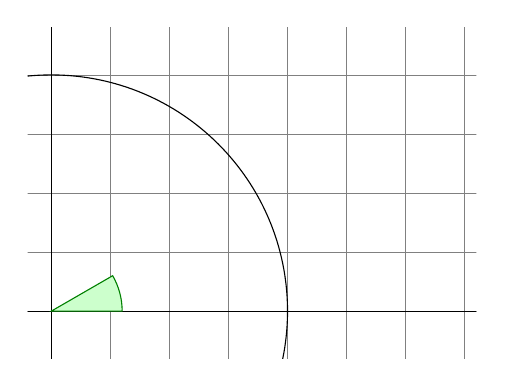
\begin{tikzpicture}[scale=3]
  \clip (-0.1,-0.2)
     rectangle (1.8,1.2);
  \draw[step=.25cm,gray,very thin]
       (-1.4,-1.4) grid (3.4,3.4);
  \draw (-1.5,0) -- (2.5,0);
  \draw (0,-1.5) -- (0,1.5);
  \draw (0,0) circle (1cm);
  \filldraw[fill=green!20!white,
            draw=green!50!black]
    (0,0) -- (3mm,0mm) 
         arc (0:30:3mm) -- cycle;
\end{tikzpicture}
\end{example}
Note the semicolon (\texttt{;}) character. It separates the individual commands.

A simple Venn diagram.
\begin{example}
\shorthandoff{:}
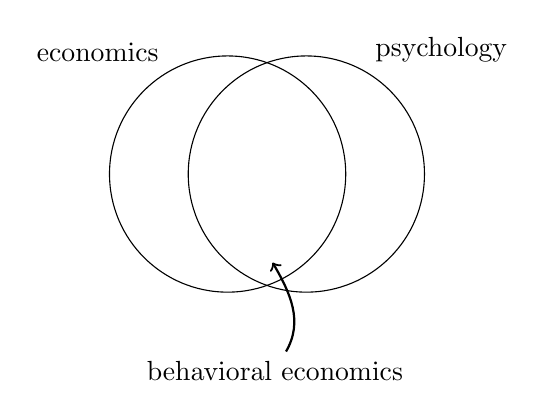
\begin{tikzpicture}
  \node[circle,draw,
        minimum size=3cm,
        label=120:{economics}]
         at (0,0) {};
  \node[circle,draw,
        minimum size=3cm,
        label=60:{psychology}]
         at (1,0) {};
  \node (i) at (0.5,-1) {};
  \node at (0.6,-2.5) 
    {behavioral economics}
    edge[->,thick,
         out=60,in=-60] (i);
\end{tikzpicture}
\end{example}
If you are using \pai{tikz} in connection with \pai{babel} some of the characters used in the
TikZ language may get modified by \pai{babel}, leading to odd errors. To counteract this, add 
the \ci{shorthandoff} command to your code.

Note the foreach loops in the next example.
\begin{example}
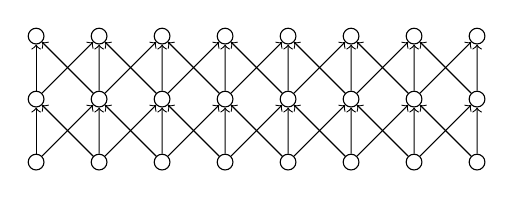
\begin{tikzpicture}[scale=0.8]
  \tikzstyle{v}=[circle, minimum size=2mm,inner sep=0pt,draw]
  \foreach \i in {1,...,8}
    \foreach \j in {1,...,3}
      \node[v] 
        (G-\i-\j) at (\i,\j) {};
  \foreach \i in {1,...,8}
    \foreach \j/\o in {1/2,2/3}
      \draw[->] 
        (G-\i-\j) -- (G-\i-\o);
  \foreach \i/\n in 
    {1/2,2/3,3/4,4/5,5/6,6/7,7/8}
    \foreach \j/\o in {1/2,2/3} {
       \draw[->] (G-\i-\j) -- (G-\n-\o);
       \draw[->] (G-\n-\j) -- (G-\i-\o);
    }
\end{tikzpicture}
\end{example}

With the \ci{usetikzlibrary}
command in the preamble you can enable a wide variety of additional
features for drawing special shapes, like this box which is slightly bent.
\begin{example}
\usetikzlibrary{%
  decorations.pathmorphing}
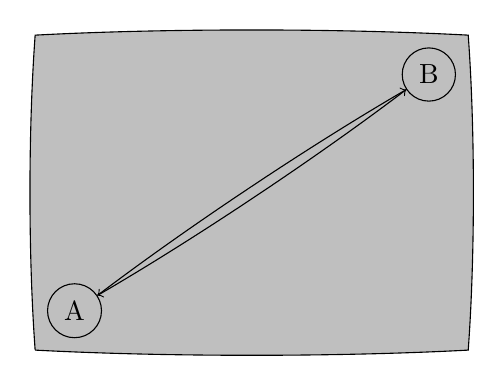
\begin{tikzpicture}[
     decoration={bent,aspect=.3}]
 \draw [decorate,fill=lightgray]
        (0,0) rectangle (5.5,4);
 \node[circle,draw] 
        (A) at (.5,.5) {A};
 \node[circle,draw] 
        (B) at (5,3.5) {B};
 \draw[->,decorate] (A) -- (B);
 \draw[->,decorate] (B) -- (A);
\end{tikzpicture}
\end{example}

\begin{example}
\usetikzlibrary{positioning}
\begin{tikzpicture}[xscale=6,
     yscale=8,>=stealth]
  \tikzstyle{v}=[circle,
     minimum size=1mm,draw,thick]
  \node[v] (a) {$1$};
  \node[v] (b) [right=of a] {$2$};
  \node[v] (c) [below=of a] {$2$};
  \node[v] (d) [below=of b] {$1$};
  \draw[thick,->] 
        (a) to node {} (c);
  \draw[thick,->] 
        (a) to node {} (d);
  \draw[thick,->] 
        (b) to node {} (d);
\end{tikzpicture}
\end{example}

You can even draw syntax diagrams that look as if they came straight from a book on
Pascal programming. The code is a bit more daunting than the example above,
so I will just show you the result. If you have a look at the \pai{pgf} documentation
you will find a detailed tutorial on drawing this exact diagram.

\begin{center}
\begin{tikzpicture}[point/.style={coordinate},thick,draw=black!50,>=stealth',
                    tip/.style={->,shorten >=1pt},every join/.style={rounded corners},
                    skip loop/.style={to path={-- ++(0,#1) -| (\tikztotarget)}},
                    hv path/.style={to path={-| (\tikztotarget)}},
                    vh path/.style={to path={|- (\tikztotarget)}},
                 terminal/.style={
            rounded rectangle,
            minimum size=6mm,
            thick,draw=black!50,
            top color=white,bottom color=black!20,
            font=\ttfamily\tiny},
                nonterminal/.style={
                       rectangle,
                       minimum size=6mm,
                       thick,
                       draw=red!50!black!50,         % 50% red and 50% black,
                       top color=white,              % a shading that is white at the top...
                       bottom color=red!50!black!20, % and something else at the bottom
                       font=\itshape\tiny}]
\matrix[column sep=4mm] {
  % First row:
  & & & & & & & & & & & \node (plus) [terminal] {+};\\
  % Second row:
  \node (p1) [point] {}; &     \node (ui1)    [nonterminal] {unsigned integer}; &
  \node (p2) [point] {}; &     \node (dot)    [terminal]    {.};                &
  \node (p3) [point] {}; &     \node (digit) [terminal]     {digit};            &
  \node (p4) [point] {}; &     \node (p5)     [point] {};                       &
  \node (p6) [point] {}; &     \node (e)      [terminal]    {E};                &
  \node (p7) [point] {}; &                                                      &
  \node (p8) [point] {}; &     \node (ui2)    [nonterminal] {unsigned integer}; &
  \node (p9) [point] {}; &     \node (p10)    [point]       {};\\
  % Third row:
  & & & & & & & & & & & \node (minus)[terminal] {-};\\
};
{ [start chain]
  \chainin (p1);
  \chainin (ui1)   [join=by tip];
  \chainin (p2)    [join];
  \chainin (dot)   [join=by tip];
  \chainin (p3)    [join];
  \chainin (digit) [join=by tip];
  \chainin (p4)    [join];
  { [start branch=digit loop]
    \chainin (p3) [join=by {skip loop=-6mm,tip}];
  }
  \chainin (p5)    [join,join=with p2 by {skip loop=6mm,tip}];
  \chainin (p6)    [join];
  \chainin (e)     [join=by tip];
  \chainin (p7)    [join];
  { [start branch=plus]
    \chainin (plus) [join=by {vh path,tip}];
    \chainin (p8)    [join=by {hv path,tip}];
  }
  { [start branch=minus]
    \chainin (minus) [join=by {vh path,tip}];
    \chainin (p8)    [join=by {hv path,tip}];
  }
  \chainin (p8)    [join];
  \chainin (ui2)   [join=by tip];
  \chainin (p9)    [join,join=with p6 by {skip loop=-11mm,tip}];
  \chainin (p10)   [join=by tip];
}
\end{tikzpicture}
\end{center}

And there is more, if you have to draw plots of numerical data or
functions, you should have a closer look at the  \pai{pgfplot}
package. It provides everything you need to draw plots. It can even
call the external \texttt{gnuplot} command to evaluate actual
functions you wrote into the graph.

For more inspiration make sure to visit Kjell Magne Fauske's excellent
\url{http://www.texample.net/tikz/}. it contains an ever expanding store of
beautiful graphs and other \LaTeX{} code. On \TeX{}ample.net you will also
find a
 \href{http://www.texample.net/tikz/resources/#tools-that-generate-pgftikz-code}{list
 of tools to work with PGF/TikZ} so that you do not have to write all that
 code by hand.

%%% Local Variables:
%%% TeX-master: "lshort.tex"
%%% mode: flyspell
%%% TeX-PDF-mode: t
%%% End:

%%%%%%%%%%%%%%%%%%%%%%%%%%%%%%%%%%%%%%%%%%%%%%%%%%%%%%%%%%%%%%%%%
% Contents: Customising LaTeX output
% $Id$
%%%%%%%%%%%%%%%%%%%%%%%%%%%%%%%%%%%%%%%%%%%%%%%%%%%%%%%%%%%%%%%%%
\chapter{Customising \LaTeX}

\begin{intro}
Documents produced with the commands you have learned up to this
point will look acceptable to a large audience. While they are not
fancy-looking, they obey all the established rules of good
typesetting, which will make them easy to read and pleasant to look at.

However, there are situations where \LaTeX{} does not provide a
command or environment that matches your needs, or the output
produced by some existing command may not meet your requirements.

In this chapter, I will try to give some hints on
how to teach \LaTeX{} new tricks and how to make it produce output
that looks different from what is provided by default.
\end{intro}


\section{New Commands, Environments and Packages}

You may have noticed that all the commands I introduce in this
book are typeset in a box, and that they show up in the index at the end
of the book. Instead of directly using the necessary \LaTeX{} commands
to achieve this, I have created a \wi{package} in which I defined new
commands and environments for this purpose. Now I can simply write:

\begin{example}
\begin{lscommand}
\ci{dum}
\end{lscommand}
\end{example}

In this example, I am using both a new environment called\\
\ei{lscommand}, which is responsible for drawing the box around the
command, and a new command named \ci{ci}, which typesets the command
name and makes a corresponding entry in the index. You can check
this out by looking up the \ci{dum} command in the index at the back
of this book, where you'll find an entry for \ci{dum}, pointing to
every page where I mentioned the \ci{dum} command.

If I ever decide that I do not like the commands to be typeset in
a box any more, I can simply change the definition of the
\texttt{lscommand} environment to create a new look. This is much
easier than going through the whole document to hunt down all the
places where I have used some generic \LaTeX{} commands to draw a
box around some word. 


\subsection{New Commands}

To add your own commands, use the
\begin{lscommand}
\ci{newcommand}\verb|{|%
       \emph{name}\verb|}[|\emph{num}\verb|]{|\emph{definition}\verb|}|
\end{lscommand}
\noindent command. 
Basically, the command requires two arguments: the \emph{name} of the
command you want to create, and the \emph{definition} of the command.
The \emph{num} argument in square brackets is optional and specifies the number
of arguments the new command takes (up to 9 are possible).
If missing it defaults to 0, i.e. no argument allowed.

The following two examples should help you to get the idea.
The first example defines a new command called \ci{tnss}. This is
short for ``The Not So Short Introduction to \LaTeXe.'' Such a command
could come in handy if you had to write the title of this book over 
and over again. 

\begin{example}
\newcommand{\tnss}{The not
    so Short Introduction to
    \LaTeXe}
This is ``\tnss'' \ldots{} 
``\tnss''
\end{example}

The next example illustrates how to define a new
command that takes one argument.
The \verb|#1| tag gets replaced by the argument you specify.
If you wanted to use more than one argument, use \verb|#2| and
so on.

\begin{example}
\newcommand{\txsit}[1]
 {This is the \emph{#1} Short 
      Introduction to \LaTeXe}
% in the document body: 
\begin{itemize}
\item \txsit{not so}
\item \txsit{very}
\end{itemize}
\end{example}

\LaTeX{} will not allow you to create a new command that would
overwrite an existing one. But there is a special command in case you
explicitly want this: \ci{renewcommand}.
It uses the same syntax as the \verb|\newcommand|
command.

In certain cases you might also want to use the \ci{providecommand}
command. It works like \ci{newcommand}, but if the command is
already defined, \LaTeXe{} will silently ignore it.

There are some points to note about whitespace following \LaTeX{} commands. See
page \pageref{whitespace} for more information.

\subsection{New Environments}
Just as with the \verb|\newcommand| command, there is a command
to create your own environments. The \ci{newenvironment} command uses the
following syntax:

\begin{lscommand}
\ci{newenvironment}\verb|{|%
       \emph{name}\verb|}[|\emph{num}\verb|]{|%
       \emph{before}\verb|}{|\emph{after}\verb|}|
\end{lscommand}

Again \ci{newenvironment} can have
an optional argument. The material specified
in the \emph{before} argument is processed before the text in the 
environment gets processed. The material in the \emph{after} argument gets
processed when the \verb|\end{|\emph{name}\verb|}| command is encountered.

The example below illustrates the usage of the \ci{newenvironment}
command. 
\begin{example}
\newenvironment{king}
 {\rule{1ex}{1ex}%
      \hspace{\stretch{1}}}
 {\hspace{\stretch{1}}%
      \rule{1ex}{1ex}}

\begin{king} 
My humble subjects \ldots
\end{king}
\end{example}

The \emph{num} argument is used the same way as in the
\verb|\newcommand| command. \LaTeX{} makes sure that you do not define
an environment that already exists. If you ever want to change an
existing command, you can use the \ci{renewenvironment} command. It
uses the same syntax as the \ci{newenvironment} command.

The commands used in this example will be explained later. For the
\ci{rule} command see page \pageref{sec:rule}, for \ci{stretch} go to
page \pageref{cmd:stretch}, and more information on \ci{hspace} can be
found on page \pageref{sec:hspace}.

\subsection{Extra Space}

When creating a new environment you may easily get bitten by extra spaces
creeping in, which can potentially have fatal effects. For example when you
want to create a title environment which supresses its own indentation as
well as the one on the following paragraph. The \ci{ignorespaces} command in
the begin block of the environment will make it ignore any space after
executing the begin block. The end block is a bit more tricky as special
processing occurs at the end of an environment. With the
\ci{ignorespacesafterend} \LaTeX{} will issue an \ci{ignorespaces} after the
special `end' processing has occured.

\begin{example}
\newenvironment{simple}%
 {\noindent}%
 {\par\noindent}

\begin{simple}
See the space\\to the left.
\end{simple}
Same\\here.
\end{example}

\begin{example}
\newenvironment{correct}%
 {\noindent\ignorespaces}%
 {\par\noindent%
   \ignorespacesafterend}

\begin{correct}
No space\\to the left.
\end{correct}
Same\\here.
\end{example}

\subsection{Commandline \LaTeX}

If you work on a Unix like OS, you might be using Makefiles to build your
\LaTeX{} projects. In that connection it might be interesting to produce
different versions of the same document by calling \LaTeX{} with commandline
parameters. If you add the following structure to your document:

\begin{verbatim}
\usepackage{ifthen}
\ifthenelse{\equal{\blackandwhite}{true}}{
  % "black and white" mode; do something..
}{
  % "color" mode; do something different..
}
\end{verbatim}

Now you can call \LaTeX{} like this:
\begin{verbatim}
latex '\newcommand{\blackandwhite}{true}\input{test.tex}'
\end{verbatim}

First the command \verb|\blackandwhite| gets defined and then the actual file is read with input.
By setting \verb|\blackandwhite| to false the color version of the document would be produced.

\subsection{Your Own Package}

If you define a lot of new environments and commands, the preamble of
your document will get quite long. In this situation, it is a good
idea to create a \LaTeX{} package containing all your command and
environment definitions. You can then use the \ci{usepackage}
command to make the package available in your document.

\begin{figure}[!htbp]
\begin{lined}{\textwidth}
\begin{verbatim}
% Demo Package by Tobias Oetiker
\ProvidesPackage{demopack}
\newcommand{\tnss}{The not so Short Introduction 
                   to \LaTeXe}
\newcommand{\txsit}[1]{The \emph{#1} Short 
                       Introduction to \LaTeXe}
\newenvironment{king}{\begin{quote}}{\end{quote}}
\end{verbatim}
\end{lined}
\caption{Example Package.} \label{package}
\end{figure}

Writing a package basically consists of copying the contents of
your document preamble into a separate file with a name ending in
\texttt{.sty}. There is one special command,
\begin{lscommand}
\ci{ProvidesPackage}\verb|{|\emph{package name}\verb|}|
\end{lscommand}
\noindent for use at the very beginning of your package
file. \verb|\ProvidesPackage| tells \LaTeX{} the name of the package
and will allow it to issue a sensible error message when you try to
include a package twice. Figure~\ref{package} shows a small example
package that contains the commands defined in the examples above.

\section{Fonts and Sizes}

\subsection{Font Changing Commands}
\index{font}\index{font size} \LaTeX{} chooses the appropriate font
and font size based on the logical structure of the document
(sections, footnotes, \ldots).  In some cases, one might like to change
fonts and sizes by hand. To do this, you can use the commands listed in
Tables~\ref{fonts} and~\ref{sizes}. The actual size of each font
is a design issue and depends on the document class and its options. 
Table~\ref{tab:pointsizes} shows the absolute point size for these
commands as implemented in the standard document classes.

\begin{example}
{\small The small and 
\textbf{bold} Romans ruled}
{\Large all of great big 
\textit{Italy}.}
\end{example}

One important feature of \LaTeXe{} is that the font attributes are
independent. This means that you can issue size or even font
changing commands, and still keep the bold or slant attribute set
earlier.

In \emph{math mode} you can use the font changing \emph{commands} to
temporarily exit \emph{math mode} and enter some normal text. If you want to
switch to another font for math typesetting you need another
special set of commands; refer to Table~\ref{mathfonts}.

\begin{table}[!bp]
\caption{Fonts.} \label{fonts}
\begin{lined}{12cm}
%
% Alan suggested not to tell about the other form of the command
% eg \verb|\sffamily| or \verb|\bfseries|. This seems a good thing to me.
%
\begin{tabular}{@{}rl@{\qquad}rl@{}}
\fni{textrm}\verb|{...}|        &      \textrm{\wi{roman}}&
\fni{textsf}\verb|{...}|        &      \textsf{\wi{sans serif}}\\
\fni{texttt}\verb|{...}|        &      \texttt{typewriter}\\[6pt]
\fni{textmd}\verb|{...}|        &      \textmd{medium}&
\fni{textbf}\verb|{...}|        &      \textbf{\wi{bold face}}\\[6pt]
\fni{textup}\verb|{...}|        &       \textup{\wi{upright}}&
\fni{textit}\verb|{...}|        &       \textit{\wi{italic}}\\
\fni{textsl}\verb|{...}|        &       \textsl{\wi{slanted}}&
\fni{textsc}\verb|{...}|        &       \textsc{\wi{Small Caps}}\\[6pt]
\ci{emph}\verb|{...}|          &            \emph{emphasized} &
\fni{textnormal}\verb|{...}|    &    \textnormal{document} font
\end{tabular}

\bigskip
\end{lined}
\end{table}


\begin{table}[!bp]
\index{font size}
\caption{Font Sizes.} \label{sizes}
\begin{lined}{12cm}
\begin{tabular}{@{}ll}
\fni{tiny}      & \tiny        tiny font \\
\fni{scriptsize}   & \scriptsize  very small font\\
\fni{footnotesize} & \footnotesize  quite small font \\
\fni{small}        &  \small            small font \\
\fni{normalsize}   &  \normalsize  normal font \\
\fni{large}        &  \large       large font
\end{tabular}%
\qquad\begin{tabular}{ll@{}}
\fni{Large}        &  \Large       larger font \\[5pt]
\fni{LARGE}        &  \LARGE       very large font \\[5pt]
\fni{huge}         &  \huge        huge \\[5pt]
\fni{Huge}         &  \Huge        largest
\end{tabular}

\bigskip
\end{lined}
\end{table}

\begin{table}[!tbp]
\caption{Absolute Point Sizes in Standard Classes.}\label{tab:pointsizes}
\label{tab:sizes}
\begin{lined}{12cm}
\begin{tabular}{lrrr}
\multicolumn{1}{c}{size} &
\multicolumn{1}{c}{10pt (default) } &
           \multicolumn{1}{c}{11pt option}  &
           \multicolumn{1}{c}{12pt option}\\
\verb|\tiny|       & 5pt  & 6pt & 6pt\\
\verb|\scriptsize| & 7pt  & 8pt & 8pt\\
\verb|\footnotesize| & 8pt & 9pt & 10pt \\
\verb|\small|        & 9pt & 10pt & 11pt \\
\verb|\normalsize| & 10pt & 11pt & 12pt \\
\verb|\large|      & 12pt & 12pt & 14pt \\
\verb|\Large|      & 14pt & 14pt & 17pt \\
\verb|\LARGE|      & 17pt & 17pt & 20pt\\
\verb|\huge|       & 20pt & 20pt & 25pt\\
\verb|\Huge|       & 25pt & 25pt & 25pt\\
\end{tabular}

\bigskip
\end{lined}
\end{table}


\begin{table}[!bp]
\caption{Math Fonts.} \label{mathfonts}
\begin{lined}{0.7\textwidth}
\begin{tabular}{@{}ll@{}}
\fni{mathrm}\verb|{...}|&     $\mathrm{Roman\ Font}$\\
\fni{mathbf}\verb|{...}|&     $\mathbf{Boldface\ Font}$\\
\fni{mathsf}\verb|{...}|&     $\mathsf{Sans\ Serif\ Font}$\\
\fni{mathtt}\verb|{...}|&     $\mathtt{Typewriter\ Font}$\\
\fni{mathit}\verb|{...}|&     $\mathit{Italic\ Font}$\\
\fni{mathcal}\verb|{...}|&    $\mathcal{CALLIGRAPHIC\ FONT}$\\
\fni{mathnormal}\verb|{...}|& $\mathnormal{Normal\ Font}$\\
\end{tabular}

%\begin{tabular}{@{}lll@{}}
%\textit{Command}&\textit{Example}&    \textit{Output}\\[6pt]
%\fni{mathcal}\verb|{...}|&    \verb|$\mathcal{B}=c$|&     $\mathcal{B}=c$\\
%\fni{mathscr}\verb|{...}|&    \verb|$\mathscr{B}=c$|&     $\mathscr{B}=c$\\
%\fni{mathrm}\verb|{...}|&     \verb|$\mathrm{K}_2$|&      $\mathrm{K}_2$\\
%\fni{mathbf}\verb|{...}|&     \verb|$\sum x=\mathbf{v}$|& $\sum x=\mathbf{v}$\\
%\fni{mathsf}\verb|{...}|&     \verb|$\mathsf{G\times R}$|&        $\mathsf{G\times R}$\\
%\fni{mathtt}\verb|{...}|&     \verb|$\mathtt{L}(b,c)$|&   $\mathtt{L}(b,c)$\\
%\fni{mathnormal}\verb|{...}|& \verb|$\mathnormal{R_{19}}\neq R_{19}$|&
%$\mathnormal{R_{19}}\neq R_{19}$\\
%\fni{mathit}\verb|{...}|&     \verb|$\mathit{ffi}\neq ffi$|& $\mathit{ffi}\neq ffi$
%\end{tabular}

\bigskip
\end{lined}
\end{table}

In connection with the font size commands, \wi{curly braces} play a
significant role. They are used to build \emph{groups}.  Groups
limit the scope of most \LaTeX{} commands.\index{grouping}

\begin{example}
He likes {\LARGE large and 
{\small small} letters}. 
\end{example}
 
The font size commands also change the line spacing, but only if the
paragraph ends within the scope of the font size command. The closing curly
brace \verb|}| should therefore not come too early.  Note the position of
the \ci{par} command in the next two examples. \footnote{\texttt{\bs{}par}
is equivalent to a blank line}


\begin{example}
{\Large Don't read this! 
 It is not true.
 You can believe me!\par}
\end{example}

\begin{example}
{\Large This is not true either.
But remember I am a liar.}\par
\end{example}

If you want to activate a size changing command for a whole paragraph
of text or even more, you might want to use the environment syntax for
font changing commands.

\begin{example}
\begin{Large} 
This is not true.
But then again, what is these
days \ldots
\end{Large}
\end{example}

\noindent This will save you from counting lots of curly braces.

\subsection{Danger, Will Robinson, Danger}

As noted at the beginning of this chapter, it is dangerous to clutter
your document with explicit commands like this, because they work in
opposition to the basic idea of \LaTeX{}, which is to separate the
logical and visual markup of your document.  This means that if you
use the same font changing command in several places in order to
typeset a special kind of information, you should use
\verb|\newcommand| to define a ``logical wrapper command'' for the font
changing command.

\begin{example}
\newcommand{\oops}[1]{%
 \textbf{#1}}
Do not \oops{enter} this room,
it's occupied by \oops{machines}
of unknown origin and purpose.
\end{example}

This approach has the advantage that you can decide at some later
stage that you want to use some visual representation of danger other
than \verb|\textbf|, without having to wade through your document,
identifying all the occurrences of \verb|\textbf| and then figuring out
for each one whether it was used for pointing out danger or for some other
reason.


\subsection{Advice}

To conclude this journey into the land of fonts and font sizes,
here is a little word of advice:\nopagebreak

\begin{quote}
  \underline{\textbf{Remember\Huge!}} \textit{The}
  \textsf{M\textbf{\LARGE O} \texttt{R}\textsl{E}} fonts \Huge you
  \tiny use \footnotesize \textbf{in} a \small \texttt{document},
  \large \textit{the} \normalsize more \textsc{readable} and
  \textsl{\textsf{beautiful} it bec\large o\Large m\LARGE e\huge s}.
\end{quote}

\section{Spacing}
 
\subsection{Line Spacing}

\index{line spacing} If you want to use larger inter-line spacing in a
document, you can change its value by putting the
\begin{lscommand}
\ci{linespread}\verb|{|\emph{factor}\verb|}|
\end{lscommand}
\noindent command into the preamble of your document.
Use \verb|\linespread{1.3}| for ``one and a half'' line
spacing, and \verb|\linespread{1.6}| for ``double'' line spacing.  Normally
the lines are not spread, so the default line spread factor
is~1.\index{double line spacing}

Note that the effect of the \ci{linespread} command is rather drastic and     
not appropriate for published work. So if you have a good reason for
changing the line spacing you might want to use the command:
\begin{lscommand}
\verb|\setlength{\baselineskip}{1.5\baselineskip}|
\end{lscommand}

\begin{example}
{\setlength{\baselineskip}%
           {1.5\baselineskip}
This paragraph is typeset with
the baseline skip set to 1.5 of
what it was before. Note the par
command at the end of the
paragraph.\par}

This paragraph has a clear
purpose, it shows that after the
curly brace has been closed,
everything is back to normal.
\end{example}

\subsection{Paragraph Formatting}\label{parsp}

In \LaTeX{}, there are two parameters influencing paragraph layout.
By placing a definition like
\begin{code}
\ci{setlength}\verb|{|\ci{parindent}\verb|}{0pt}| \\
\verb|\setlength{|\ci{parskip}\verb|}{1ex plus 0.5ex minus 0.2ex}|
\end{code}
in the preamble of the input file, you can change the layout of
paragraphs. These two commands increase the space between two paragraphs
while setting the paragraph indent to zero.  

The \texttt{plus} and \texttt{minus} parts of the length above tell
\TeX{} that it can compress and expand the inter paragraph skip by the
amount specified, if this is necessary to properly fit the paragraphs
onto the page.

In continental Europe,
paragraphs are often separated by some space and not indented. But
beware, this also has its effect on the table of contents. Its lines
get spaced more loosely now as well. To avoid this, you might want to
move the two commands from the preamble into your document to some
place below the command \verb|\tableofcontents| or to not use them at all,
because you'll find that most professional books use indenting and not
spacing to separate paragraphs.


If you want to indent a paragraph that is not indented, you can use 
\begin{lscommand}
\ci{indent}
\end{lscommand}
\noindent at the beginning of the paragraph.\footnote{To indent the first paragraph after each section head, use
  the \pai{indentfirst} package in the `tools' bundle.} Obviously,
this will only have an effect when \verb|\parindent| is not set to
zero.

To create a non-indented paragraph, you can use 
\begin{lscommand}
\ci{noindent}
\end{lscommand}
\noindent as the first command of the paragraph. This might come in handy when
you start a document with body text and not with a sectioning command.

\subsection{Horizontal Space}

\label{sec:hspace}
\LaTeX{} determines the spaces between words and sentences
automatically. To add horizontal space, use: \index{horizontal!space}
\begin{lscommand}
\ci{hspace}\verb|{|\emph{length}\verb|}|
\end{lscommand}
If such a space should be kept even if it falls at the end or the
start of a line, use \verb|\hspace*| instead of \verb|\hspace|.  The
\emph{length} in the simplest case is just a number plus a unit.  The
most important units are listed in Table~\ref{units}. 
\index{units}\index{dimensions}

\begin{example}
This\hspace{1.5cm}is a space 
of 1.5 cm. 
\end{example}
\suppressfloats
\begin{table}[tbp]
\caption{\TeX{} Units.} \label{units}\index{units}
\begin{lined}{9.5cm} 
\begin{tabular}{@{}ll@{}}
\texttt{mm} & millimetre $\approx 1/25$~inch \quad \demowidth{1mm} \\
\texttt{cm} & centimetre = 10~mm  \quad \demowidth{1cm}                     \\
\texttt{in} & inch $=$ 25.4~mm \quad \demowidth{1in}                    \\
\texttt{pt} & point $\approx 1/72$~inch $\approx \frac{1}{3}$~mm  \quad\demowidth{1pt}\\
\texttt{em} & approx width of an `M' in the current font \quad \demowidth{1em}\\
\texttt{ex} & approx height of an `x' in the current font \quad \demowidth{1ex}
\end{tabular}

\bigskip
\end{lined}
\end{table}

\label{cmd:stretch} 
The command
\begin{lscommand}
\ci{stretch}\verb|{|\emph{n}\verb|}|
\end{lscommand} 
\noindent generates a special rubber space. It stretches until all the
remaining space on a line is filled up. If multiple
\verb|\hspace{\stretch{|\emph{n}\verb|}}| commands are issued on the same
line, they occupy all available space in proportion of their respective
stretch factors.


\begin{example}
x\hspace{\stretch{1}}
x\hspace{\stretch{3}}x
\end{example}

When using horizontal space together with text, it may make sense to make
the space adjust its size relative to the size of the current font.
This can be done by using the text-relative units \texttt{em} and
\texttt{ex}:

\begin{example}
{\Large{}big\hspace{1em}y}\\
{\tiny{}tin\hspace{1em}y}
\end{example}
 
\subsection{Vertical Space}
The space between paragraphs, sections, subsections, \ldots\ is
determined automatically by \LaTeX. If necessary, additional vertical
space \emph{between two paragraphs} can be added with the command:
\begin{lscommand}
\ci{vspace}\verb|{|\emph{length}\verb|}|
\end{lscommand}

This command should normally be used between two empty lines.  If the
space should be preserved at the top or at the bottom of a page, use
the starred version of the command, \verb|\vspace*|, instead of \verb|\vspace|.
\index{vertical space}

The \verb|\stretch| command, in connection with \verb|\pagebreak|, can
be used to typeset text on the last line of a page, or to centre text
vertically on a page.
\begin{code}
\begin{verbatim}
Some text \ldots

\vspace{\stretch{1}}
This goes onto the last line of the page.\pagebreak
\end{verbatim}
\end{code}

Additional space between two lines of \emph{the same} paragraph or
within a table is specified with the
\begin{lscommand}
\ci{\bs}\verb|[|\emph{length}\verb|]|
\end{lscommand}
\noindent command. 

With \ci{bigskip} and \ci{smallskip} you can skip a predefined amount of
vertical space without having to worry about exact numbers.


\section{Page Layout}

\begin{figure}[!hp]
\begin{center}
\makeatletter\@mylayout\makeatother
\end{center}
\vspace*{1.8cm}
\caption{Page Layout Parameters.}
\label{fig:layout}
\cih{footskip}
\cih{headheight}
\cih{headsep}
\cih{marginparpush}
\cih{marginparsep}
\cih{marginparwidth}
\cih{oddsidemargin}
\cih{paperheight}
\cih{paperwidth}
\cih{textheight}
\cih{textwidth}
\cih{topmargin}
\end{figure}
\index{page layout}
\LaTeXe{} allows you to specify the \wi{paper size} in the
\verb|\documentclass| command. It then automatically picks the right 
text \wi{margins}, but sometimes you may not be happy with 
the predefined values. Naturally, you can change them. 
%no idea why this is needed here ...
\thispagestyle{fancyplain}
Figure~\ref{fig:layout} shows all the parameters that can be changed.
The figure was produced with the \pai{layout} package from the tools bundle.%
\footnote{\CTANref|macros/latex/required/tools|}

\textbf{WAIT!} \ldots before you launch into a ``Let's make that
narrow page a bit wider'' frenzy, take a few seconds to think. As with
most things in \LaTeX, there is a good reason for the page layout to
be as it is.

Sure, compared to your off-the-shelf MS Word page, it looks awfully
narrow. But take a look at your favourite book\footnote{I mean a real
  printed book produced by a reputable publisher.} and count the number
of characters on a standard text line. You will find that there are no
more than about 66 characters on each line. Now do the same on your
\LaTeX{} page. You will find that there are also about 66 characters
per line.  Experience shows that the reading gets difficult as soon as
there are more characters on a single line. This is because it is
difficult for the eyes to move from the end of one line to the start of the next one.
This is also why newspapers are typeset in multiple columns.

So if you increase the width of your body text, keep in mind that you
are making life difficult for the readers of your paper. But enough
of the cautioning, I promised to tell you how you do it \ldots
 
\LaTeX{} provides two commands to change these parameters. They are
usually used in the document preamble.

The first command assigns a fixed value to any of the parameters:
\begin{lscommand}
\ci{setlength}\verb|{|\emph{parameter}\verb|}{|\emph{length}\verb|}|
\end{lscommand}

The second command adds a length to any of the parameters:
\begin{lscommand}
\ci{addtolength}\verb|{|\emph{parameter}\verb|}{|\emph{length}\verb|}|
\end{lscommand} 

This second command is actually more useful than the \ci{setlength}
command, because you can now work relative to the existing settings.
To add one centimetre to the overall text width, I put the
following commands into the document preamble:
\begin{code}
\verb|\addtolength{\hoffset}{-0.5cm}|\\
\verb|\addtolength{\textwidth}{1cm}|
\end{code}

In this context, you might want to look at the \pai{calc} package.
It allows you to use arithmetic operations in the argument of \ci{setlength}
and other places where you can enter numeric values into function
arguments.

\section{More Fun With Lengths}

Whenever possible, I avoid using absolute lengths in
\LaTeX{} documents. I rather try to base things on the width or height
of other page elements. For the width of a figure this could
be \verb|\textwidth| in order to make it fill the page.

The following 3 commands allow you to determine the width, height and
depth of a text string.

\begin{lscommand}
\ci{settoheight}\verb|{|\emph{variable}\verb|}{|\emph{text}\verb|}|\\
\ci{settodepth}\verb|{|\emph{variable}\verb|}{|\emph{text}\verb|}|\\
\ci{settowidth}\verb|{|\emph{variable}\verb|}{|\emph{text}\verb|}|
\end{lscommand}

\noindent The example below shows a possible application of these commands.

\begin{example}
\flushleft
\newenvironment{vardesc}[1]{%
  \settowidth{\parindent}{#1:\ }
  \makebox[0pt][r]{#1:\ }}{}

\begin{displaymath}
a^2+b^2=c^2
\end{displaymath}

\begin{vardesc}{Where}$a$, 
$b$ -- are adjoin to the right 
angle of a right-angled triangle.  

$c$ -- is the hypotenuse of 
the triangle and feels lonely.

$d$ -- finally does not show up 
here at all. Isn't that puzzling?
\end{vardesc}
\end{example}

\section{Boxes}
\LaTeX{} builds up its pages by pushing around boxes. At first, each
letter is a little box, which is then glued to other letters to form
words. These are again glued to other words, but with special glue,
which is elastic so that a series of words can be squeezed or
stretched as to exactly fill a line on the page. 

I admit, this is a very simplistic version of what really happens, but
the point is that \TeX{} operates on glue and boxes. Letters are not the only things that
can be boxes. You can put virtually everything into a box, including
other boxes. Each box will then be handled by \LaTeX{} as if it were a
single letter.

In the past chapters you have already encountered some boxes, although
I did not tell you. The \ei{tabular} environment and the
\ci{includegraphics}, for example, both produce a box. This means that you can
easily arrange two tables or images side by side. You just have to
make sure that their combined width is not larger than the textwidth.

You can also pack a paragraph of your choice into a box with either
the

\begin{lscommand}
\ci{parbox}\verb|[|\emph{pos}\verb|]{|\emph{width}\verb|}{|\emph{text}\verb|}|
\end{lscommand}

\noindent command or the

\begin{lscommand}
\verb|\begin{|\ei{minipage}\verb|}[|\emph{pos}\verb|]{|\emph{width}\verb|}| text
\verb|\end{|\ei{minipage}\verb|}|
\end{lscommand}

\noindent environment. The \texttt{pos} parameter can take one of the letters
\texttt{c, t} or \texttt{b} to control the vertical alignment of the box,
relative to the baseline of the surrounding text. \texttt{width} takes
a length argument specifying the width of the box. The main difference
between a \ei{minipage} and a \ci{parbox} is that you cannot use all commands
and environments inside a \ei{parbox}, while almost anything is possible in
a \ei{minipage}.

While \ci{parbox} packs up a whole paragraph doing line breaking and
everything, there is also a class of boxing commands that operates
only on horizontally aligned material. We already know one of them;
it's called \ci{mbox}. It simply packs up a series of boxes into
another one, and can be used to prevent \LaTeX{} from breaking two
words. As you can put boxes inside boxes, these horizontal box packers
give you ultimate flexibility.

\begin{lscommand}
\ci{makebox}\verb|[|\emph{width}\verb|][|\emph{pos}\verb|]{|\emph{text}\verb|}|
\end{lscommand}

\noindent \texttt{width} defines the width of the resulting box as
seen from the outside.\footnote{This means it can be smaller than the
material inside the box. You can even set the
width to 0pt so that the text inside the box will be typeset without
influencing the surrounding boxes.}  Besides the length
expressions, you can also use \ci{width}, \ci{height}, \ci{depth}, and
\ci{totalheight} in the width parameter. They are set from values
obtained by measuring the typeset \emph{text}. The \emph{pos} parameter takes
a one letter value: \textbf{c}enter, flush\textbf{l}eft,
flush\textbf{r}ight, or \textbf{s}pread the text to fill the box.

The command \ci{framebox} works exactly the same as \ci{makebox}, but
it draws a box around the text.

The following example shows you some things you could do with
the \ci{makebox} and \ci{framebox} commands.

\begin{example}
\makebox[\textwidth]{%
    c e n t r a l}\par
\makebox[\textwidth][s]{%
    s p r e a d}\par
\framebox[1.1\width]{Guess I'm 
    framed now!} \par
\framebox[0.8\width][r]{Bummer, 
    I am too wide} \par
\framebox[1cm][l]{never 
    mind, so am I} 
Can you read this?
\end{example}

Now that we control the horizontal, the obvious next step is to go for
  the vertical.\footnote{Total control is only to be obtained by
  controlling both the horizontal and the vertical \ldots}
 No problem for \LaTeX{}. The


\begin{lscommand}
\ci{raisebox}\verb|{|\emph{lift}\verb|}[|\emph{extend-above-baseline}\verb|][|\emph{extend-below-baseline}\verb|]{|\emph{text}\verb|}|
\end{lscommand}

\noindent command lets you define the vertical properties of a
box. You can use \ci{width}, \ci{height}, \ci{depth}, and
  \ci{totalheight} in the first three parameters, in order to act
  upon the size of the box inside the \emph{text} argument.


\begin{example}
\raisebox{0pt}[0pt][0pt]{\Large%
\textbf{Aaaa\raisebox{-0.3ex}{a}%
\raisebox{-0.7ex}{aa}%
\raisebox{-1.2ex}{r}%
\raisebox{-2.2ex}{g}%
\raisebox{-4.5ex}{h}}}
she shouted, but not even the next
one in line noticed that something
terrible had happened to her.
\end{example}

\section{Rules and Struts}
\label{sec:rule}

A few pages back you may have noticed the command

\begin{lscommand}
\ci{rule}\verb|[|\emph{lift}\verb|]{|\emph{width}\verb|}{|\emph{height}\verb|}|
\end{lscommand}

\noindent In normal use it produces a simple black box.

\begin{example}
\rule{3mm}{.1pt}%
\rule[-1mm]{5mm}{1cm}%
\rule{3mm}{.1pt}%
\rule[1mm]{1cm}{5mm}%
\rule{3mm}{.1pt}
\end{example}

\noindent This is useful for drawing vertical and horizontal
lines. The line on the title page, for example, has been created with a
\ci{rule} command.

\bigskip
{\flushright The End.\par}

%

% Local Variables:
% TeX-master: "lshort2e"
% mode: latex
% mode: flyspell
% End:

\appendix
\chapter{Installing \LaTeX}
\begin{intro}
Knuth published the source to \TeX{} back in a time when nobody knew
about OpenSource and/or Free Software. The License that comes with \TeX{}
lets you do whatever you want with the source, but you can only call the
result of your work \TeX{} if the program passes a set of tests Knuth has
also provided. This has lead to a situation where we have free \TeX{}
implementations for almost every Operating System under the sun. This chapter
will give some hints on what to install on Linux, Mac OS X and Windows, to
get a working \TeX{} setup.
\end{intro}

\section{What to Install}

To use \LaTeX{} on any computer system, you need several programs.

\begin{enumerate}

\item The \TeX{}/\LaTeX{} program for processing your \LaTeX{} source files
into typeset PDF or DVI documents.

\item A text editor for editing your \LaTeX{} source files. Some products even let
you start the \LaTeX{} program from within the editor.

\item A PDF/DVI viewer program for previewing and printing your
documents.

\item A program to handle \PSi{} files and images for inclusion into
your documents.

\end{enumerate}

For every platforms there are several programs that fit the requirements above.
Here we just tell about the ones we know, like and have some experience
with.

\section{Cross Platform Editor}
\label{sec:texmaker}

While \TeX{} is available on many different computing platforms, \LaTeX{}
editors have long been highly platform specific.

Over the past few years I have come to like Texmaker quite a lot.
Apart from being very a useful editor with integrated pdf-preview and syntax
high-lighting, it has the advantage of running on Windows, Mac and
Unix/Linux equally well.  See \url{http://www.xm1math.net/texmaker} for
further information.  There is also a forked version of Texmaker called
TeXstudio on \url{http://texstudio.sourceforge.net/}.  It also seems well
maintained and is also available for all three major platforms.

You will find some platform specific editor suggestions in the OS sections
below.

\section{\TeX{} on Mac OS X}

\subsection{\TeX{} Distribution}

Just download \wi{MacTeX}. It is a
pre-compiled \LaTeX{} distribution for OS X. \wi{MacTeX} provides a full \LaTeX{}
installation plus a number of additional tools. Get Mac\TeX{} from
\url{http://www.tug.org/mactex/}.

\subsection{OSX \TeX{} Editor}

If you are not happy with our cross-platform suggestion Texmaker (section \ref{sec:texmaker}).
 
The most popular open source editor for \LaTeX{} on the mac seems to be
\TeX{}shop.  Get a copy from \url{http://www.uoregon.edu/~koch/texshop}. It
is also contained in the \wi{MacTeX} distribution.

Recent \TeX Live distributions contain the \TeX{}works editor 
\url{http://texworks.org/} which is a multi-platform editor based on the \TeX{}Shop
design. Since \TeX{}works uses the Qt toolkit, it is available on any platform
supported by this toolkit (MacOS X, Windows, Linux.) 

\subsection{Treat yourself to \wi{PDFView}}

Use PDFView for viewing PDF files generated by \LaTeX{}, it integrates tightly
with your \LaTeX{} text editor. PDFView is an open-source application, available from the PDFView website on\\
\url{http://pdfview.sourceforge.net/}. After installing, open
PDFViews preferences dialog and make sure that the \emph{automatically reload
documents} option is enabled and that PDFSync support is set appropriately.

\section{\TeX{} on Windows}

\subsection{Getting \TeX{}}

First, get a copy of the excellent MiK\TeX\index{MiKTeX@MiK\TeX} distribution from\\
\url{http://www.miktex.org/}. It contains all the basic programs and files
required to compile \LaTeX{} documents.  The coolest feature in my eyes, is
that MiK\TeX{} will download missing \LaTeX{} packages on the fly and install them
magically while compiling a document. Alternatively you can also use
the TeXlive distribution which exists for Windows, Unix and Mac OS to
get your base setup going \url{http://www.tug.org/texlive/}.

\subsection{A \LaTeX{} editor}

If you are not happy with our crossplatform suggestion Texmaker (section \ref{sec:texmaker}).

\wi{TeXnicCenter} uses many concepts from the programming-world to provide a nice and
efficient \LaTeX{} writing environment in Windows. Get your copy from\\
\url{http://www.texniccenter.org/}. TeXnicCenter integrates nicely with
MiKTeX.

Recent \TeX Live distributions contain the \TeX{}works Editor
\url{http://texworks.org/}. It supports Unicode and requires at least Windows XP.

\subsection{Document Preview}

You will most likely be using Yap for DVI preview as it gets installed with
MikTeX. For PDF you may want to look at Sumatra
PDF \url{http://blog.kowalczyk.info/software/sumatrapdf/}. I mention Sumatra PDF
because it lets you jump from any position in the pdf document back into
corresponding position in your source document.

\subsection{Working with graphics}

Working with high quality graphics in \LaTeX{} means that you have to use
\EPSi{} (eps) or PDF as your picture format. The program that helps you
deal with this is called \wi{GhostScript}. You can get it, together with its
own front-end \wi{GhostView}, from \url{http://www.cs.wisc.edu/~ghost/}.

If you deal with bitmap graphics (photos and scanned material), you may want
to have a look at the open source Photoshop alternative \wi{Gimp}, available
from \url{http://gimp-win.sourceforge.net/}.

\section{\TeX{} on Linux}

If you work with Linux, chances are high that \LaTeX{} is already installed
on your system, or at least available on the installation source you used to
setup. Use your package manager to install the following packages:

\begin{itemize}
\item texlive -- the base \TeX{}/\LaTeX{} setup.
\item emacs (with AUCTeX) -- an editor that integrates tightly with \LaTeX{} through the add-on AUCTeX package.
\item ghostscript -- a \PSi{} preview program.
\item xpdf and acrobat -- a PDF preview program.
\item imagemagick -- a free program for converting bitmap images.
\item gimp -- a free Photoshop look-a-like.
\item inkscape -- a free illustrator/corel draw look-a-like.
\end{itemize}

If you are looking for a more windows like graphical editing environment,
check out Texmaker. See section \ref{sec:texmaker}.

Most Linux distros insist on splitting up their \TeX{} environments into a
large number of optional packages, so if something is missing after your
first install, go check again.

\backmatter
%%%%%%%%%%%%%%%%%%%%%%%%%%%%%%%%%%%%%%%%%%%%%%%%%%%%%%%%%%%%%%%%%
% Contents: The Bibliography
% File: biblio.tex (lshort2e.tex)
% $Id$
%%%%%%%%%%%%%%%%%%%%%%%%%%%%%%%%%%%%%%%%%%%%%%%%%%%%%%%%%%%%%%%%%
\begin{thebibliography}{99}
\addcontentsline{toc}{chapter}{\bibname} 
\bibitem{manual} Leslie Lamport.  \newblock \emph{{\LaTeX:} A Document
    Preparation System}.  \newblock Addison-Wesley, Reading,
  Massachusetts, second edition, 1994, ISBN~0-201-52983-1.
  
\bibitem{texbook} Donald~E. Knuth.  \newblock \textit{The \TeX{}book,}
  Volume~A of \textit{Computers and Typesetting}, Addison-Wesley,
  Reading, Massachusetts, second edition, 1984, ISBN~0-201-13448-9.

\bibitem{companion} Frank Mittelbach, Michel Goossens, Johannes Braams,
  David Carlisle, Chris Rowley.  \newblock \emph{The {\LaTeX} Companion, (2nd Edition)}.  \newblock
  Addison-Wesley, Reading, Massachusetts, 2004, ISBN~0-201-36299-6.

\bibitem{graphicscompanion} Michel Goossens, Sebastian Rahtz and Frank
  Mittelbach.  \newblock \emph{The {\LaTeX} Graphics Companion}.  \newblock
  Addison-Wesley, Reading, Massachusetts, 1997, ISBN~0-201-85469-4.
 
\bibitem{local} Each \LaTeX{} installation should provide a so-called
  \emph{\LaTeX{} Local Guide}, which explains the things that are
  special to the local system.  It should be contained in a file called
  \texttt{local.tex}. Unfortunately, some lazy sysops do not provide such a
  document. In this case, go and ask your local \LaTeX{} guru for help.
 
\bibitem{usrguide} \LaTeX3 Project Team.  \newblock \emph{\LaTeXe~for
    authors}.  \newblock Comes with the \LaTeXe{} distribution as
  \texttt{usrguide.tex}.

\bibitem{clsguide} \LaTeX3 Project Team.  \newblock \emph{\LaTeXe~for
    Class and Package writers}.  \newblock Comes with the \LaTeXe{}
  distribution as \texttt{clsguide.tex}.

\bibitem{fntguide} \LaTeX3 Project Team.  \newblock \emph{\LaTeXe~Font
    selection}.  \newblock Comes with the \LaTeXe{} distribution as
  \texttt{fntguide.tex}.

\bibitem{graphics} D.~P.~Carlisle.  \newblock \emph{Packages in the
    `graphics' bundle}.  \newblock Comes with the `graphics' bundle as
  \texttt{grfguide.tex}, available from the same source your \LaTeX{}
  distribution came from.

\bibitem{verbatim} Rainer~Sch\"opf, Bernd~Raichle, Chris~Rowley.  
\newblock \emph{A New Implementation of \LaTeX's verbatim
  Environments}.
 \newblock Comes with the `tools' bundle as
  \texttt{verbatim.dtx}, available from the same source your \LaTeX{}
  distribution came from. 

\bibitem{cyrguide} Vladimir Volovich, Werner Lemberg and \LaTeX3 Project Team.                    
    \newblock \emph{Cyrillic languages support in \LaTeX}.                                        
    \newblock Comes with the \LaTeXe{} distribution as                                            
  \texttt{cyrguide.tex}.                                                                          

\bibitem{catalogue} Graham~Williams.  \newblock \emph{The TeX
    Catalogue} is a very complete listing of many \TeX{} and \LaTeX{}
    related packages.
  \newblock Available online from \CTAN|help/Catalogue/catalogue.html|
  
\bibitem{eps} Keith~Reckdahl.  \newblock \emph{Using EPS Graphics in
    \LaTeXe{} Documents}, which explains everything and much more than
  you ever wanted to know about EPS files and their use in \LaTeX{}
  documents.  \newblock Available online from
  \CTAN|info/epslatex.ps|

\bibitem{xy-pic} Kristoffer H. Rose.
  \newblock \emph{\Xy-pic User's Guide}.  \newblock
  Downloadable from CTAN with \Xy-pic distribution 
  
\bibitem{metapost} John D. Hobby.
  \newblock \emph{A User's Manual for \MP}. \newblock
  Downloadable from \url{http://cm.bell-labs.com/who/hobby/} 
  
\bibitem{unbound} Alan Hoenig.
  \newblock \emph{\TeX{} Unbound}. \newblock Oxford University Press, 1998,
    ISBN 0-19-509685-1; 0-19-509686-X (pbk.) 
  
\bibitem{ursoswald} Urs Oswald.  
    \newblock \emph{Graphics in \LaTeXe{}}, containing some Java source files for 
    generating arbitrary circles and ellipses within the \texttt{picture} environment,
    and \emph{\MP{} - A Tutorial}.
  \newblock Both downloadable from \url{http://www.ursoswald.ch}

\bibitem{pgfplots} Till Tantau.
  \newblock \emph{TikZ\&PGF Manual}.\newblock
  Download from \CTAN|graphics/pgf/base/doc/generic/pgf/pgfmanual.pdf|
  
  

\end{thebibliography}


%

% Local Variables:
% TeX-master: "lshort2e"
% mode: latex
% mode: flyspell
% End:

\refstepcounter{chapter}
\addcontentsline{toc}{chapter}{Index} 
\printindex
\end{document}





%

% Local Variables:
% TeX-master: "lshort2e"
% mode: latex
% mode: flyspell
% End:
